\documentclass[review,authoryear]{elsarticle}
%DIF LATEXDIFF DIFFERENCE FILE
%DIF DEL paper-odca-des-prerevision-2.tex   Sun Sep 20 03:44:19 2026
%DIF ADD paper-odca-des.tex                 Sun Sep 20 14:31:35 2026

\usepackage[margin=2cm]{geometry}
\usepackage{amsmath,amssymb,amsfonts}
\usepackage{graphicx}
\usepackage{booktabs}
\usepackage{multirow}
\usepackage{xcolor}
\usepackage{hyperref}
\usepackage{subcaption}
%DIF 11a11
\usepackage[section]{placeins}   % a float never crosses into the next section %DIF > 
%DIF -------
\usepackage{tikz}
\usetikzlibrary{arrows.meta,positioning,fit,backgrounds,shapes.geometric,calc}

% Notation shortcuts
\newcommand{\Treq}{T^{\text{req}}}
\newcommand{\Tacq}{T^{\text{acq}}}
\newcommand{\Tarr}{T^{\text{arr}}}
\newcommand{\Trel}{T^{\text{rel}}}

\journal{Transportation Research Part B: Methodological}
%DIF PREAMBLE EXTENSION ADDED BY LATEXDIFF
%DIF UNDERLINE PREAMBLE %DIF PREAMBLE
\RequirePackage[normalem]{ulem} %DIF PREAMBLE
\RequirePackage{color}\definecolor{RED}{rgb}{1,0,0}\definecolor{BLUE}{rgb}{0,0,1} %DIF PREAMBLE
\providecommand{\DIFaddtex}[1]{{\protect\color{blue}\uwave{#1}}} %DIF PREAMBLE
\providecommand{\DIFdeltex}[1]{{\protect\color{red}\sout{#1}}}                      %DIF PREAMBLE
%DIF SAFE PREAMBLE %DIF PREAMBLE
\providecommand{\DIFaddbegin}{} %DIF PREAMBLE
\providecommand{\DIFaddend}{} %DIF PREAMBLE
\providecommand{\DIFdelbegin}{} %DIF PREAMBLE
\providecommand{\DIFdelend}{} %DIF PREAMBLE
\providecommand{\DIFmodbegin}{} %DIF PREAMBLE
\providecommand{\DIFmodend}{} %DIF PREAMBLE
%DIF FLOATSAFE PREAMBLE %DIF PREAMBLE
\providecommand{\DIFaddFL}[1]{\DIFadd{#1}} %DIF PREAMBLE
\providecommand{\DIFdelFL}[1]{\DIFdel{#1}} %DIF PREAMBLE
\providecommand{\DIFaddbeginFL}{} %DIF PREAMBLE
\providecommand{\DIFaddendFL}{} %DIF PREAMBLE
\providecommand{\DIFdelbeginFL}{} %DIF PREAMBLE
\providecommand{\DIFdelendFL}{} %DIF PREAMBLE
%DIF HYPERREF PREAMBLE %DIF PREAMBLE
\providecommand{\DIFadd}[1]{\texorpdfstring{\DIFaddtex{#1}}{#1}} %DIF PREAMBLE
\providecommand{\DIFdel}[1]{\texorpdfstring{\DIFdeltex{#1}}{}} %DIF PREAMBLE
\newcommand{\DIFscaledelfig}{0.5}
%DIF HIGHLIGHTGRAPHICS PREAMBLE %DIF PREAMBLE
\RequirePackage{settobox} %DIF PREAMBLE
\RequirePackage{letltxmacro} %DIF PREAMBLE
\newsavebox{\DIFdelgraphicsbox} %DIF PREAMBLE
\newlength{\DIFdelgraphicswidth} %DIF PREAMBLE
\newlength{\DIFdelgraphicsheight} %DIF PREAMBLE
% store original definition of \includegraphics %DIF PREAMBLE
\LetLtxMacro{\DIFOincludegraphics}{\includegraphics} %DIF PREAMBLE
\newcommand{\DIFaddincludegraphics}[2][]{{\color{blue}\fbox{\DIFOincludegraphics[#1]{#2}}}} %DIF PREAMBLE
\newcommand{\DIFdelincludegraphics}[2][]{% %DIF PREAMBLE
\sbox{\DIFdelgraphicsbox}{\DIFOincludegraphics[#1]{#2}}% %DIF PREAMBLE
\settoboxwidth{\DIFdelgraphicswidth}{\DIFdelgraphicsbox} %DIF PREAMBLE
\settoboxtotalheight{\DIFdelgraphicsheight}{\DIFdelgraphicsbox} %DIF PREAMBLE
\scalebox{\DIFscaledelfig}{% %DIF PREAMBLE
\parbox[b]{\DIFdelgraphicswidth}{\usebox{\DIFdelgraphicsbox}\\[-\baselineskip] \rule{\DIFdelgraphicswidth}{0em}}\llap{\resizebox{\DIFdelgraphicswidth}{\DIFdelgraphicsheight}{% %DIF PREAMBLE
\setlength{\unitlength}{\DIFdelgraphicswidth}% %DIF PREAMBLE
\begin{picture}(1,1)% %DIF PREAMBLE
\thicklines\linethickness{2pt} %DIF PREAMBLE
{\color[rgb]{1,0,0}\put(0,0){\framebox(1,1){}}}% %DIF PREAMBLE
{\color[rgb]{1,0,0}\put(0,0){\line( 1,1){1}}}% %DIF PREAMBLE
{\color[rgb]{1,0,0}\put(0,1){\line(1,-1){1}}}% %DIF PREAMBLE
\end{picture}% %DIF PREAMBLE
}\hspace*{3pt}}} %DIF PREAMBLE
} %DIF PREAMBLE
\LetLtxMacro{\DIFOaddbegin}{\DIFaddbegin} %DIF PREAMBLE
\LetLtxMacro{\DIFOaddend}{\DIFaddend} %DIF PREAMBLE
\LetLtxMacro{\DIFOdelbegin}{\DIFdelbegin} %DIF PREAMBLE
\LetLtxMacro{\DIFOdelend}{\DIFdelend} %DIF PREAMBLE
\DeclareRobustCommand{\DIFaddbegin}{\DIFOaddbegin \let\includegraphics\DIFaddincludegraphics} %DIF PREAMBLE
\DeclareRobustCommand{\DIFaddend}{\DIFOaddend \let\includegraphics\DIFOincludegraphics} %DIF PREAMBLE
\DeclareRobustCommand{\DIFdelbegin}{\DIFOdelbegin \let\includegraphics\DIFdelincludegraphics} %DIF PREAMBLE
\DeclareRobustCommand{\DIFdelend}{\DIFOaddend \let\includegraphics\DIFOincludegraphics} %DIF PREAMBLE
\LetLtxMacro{\DIFOaddbeginFL}{\DIFaddbeginFL} %DIF PREAMBLE
\LetLtxMacro{\DIFOaddendFL}{\DIFaddendFL} %DIF PREAMBLE
\LetLtxMacro{\DIFOdelbeginFL}{\DIFdelbeginFL} %DIF PREAMBLE
\LetLtxMacro{\DIFOdelendFL}{\DIFdelendFL} %DIF PREAMBLE
\DeclareRobustCommand{\DIFaddbeginFL}{\DIFOaddbeginFL \let\includegraphics\DIFaddincludegraphics} %DIF PREAMBLE
\DeclareRobustCommand{\DIFaddendFL}{\DIFOaddendFL \let\includegraphics\DIFOincludegraphics} %DIF PREAMBLE
\DeclareRobustCommand{\DIFdelbeginFL}{\DIFOdelbeginFL \let\includegraphics\DIFdelincludegraphics} %DIF PREAMBLE
\DeclareRobustCommand{\DIFdelendFL}{\DIFOaddendFL \let\includegraphics\DIFOincludegraphics} %DIF PREAMBLE
%DIF COLORLISTINGS PREAMBLE %DIF PREAMBLE
\RequirePackage{listings} %DIF PREAMBLE
\RequirePackage{color} %DIF PREAMBLE
\lstdefinelanguage{DIFcode}{ %DIF PREAMBLE
%DIF DIFCODE_UNDERLINE %DIF PREAMBLE
  moredelim=[il][\color{red}\sout]{\%DIF\ <\ }, %DIF PREAMBLE
  moredelim=[il][\color{blue}\uwave]{\%DIF\ >\ } %DIF PREAMBLE
} %DIF PREAMBLE
\lstdefinestyle{DIFverbatimstyle}{ %DIF PREAMBLE
	language=DIFcode, %DIF PREAMBLE
	basicstyle=\ttfamily, %DIF PREAMBLE
	columns=fullflexible, %DIF PREAMBLE
	keepspaces=true %DIF PREAMBLE
} %DIF PREAMBLE
\lstnewenvironment{DIFverbatim}{\lstset{style=DIFverbatimstyle}}{} %DIF PREAMBLE
\lstnewenvironment{DIFverbatim*}{\lstset{style=DIFverbatimstyle,showspaces=true}}{} %DIF PREAMBLE
%DIF END PREAMBLE EXTENSION ADDED BY LATEXDIFF


% Marked build only: a revised table carries old and new in one cell, so shrink it to fit.
\usepackage{adjustbox}
\let\ODCAtabular\tabular
\let\endODCAtabular\endtabular
\renewenvironment{tabular}[2][c]{%
  \begin{adjustbox}{max width=\textwidth}\ODCAtabular[#1]{#2}%
}{%
  \endODCAtabular\end{adjustbox}%
}
% A deleted inline formula is one unbreakable box inside \sout and runs off the
% page; let TeX break inline math at relations and binary operators instead.
\relpenalty=0
\binoppenalty=0
\setlength{\emergencystretch}{3em}
% The marked builds cite their own bibliography: references.bib plus the entries
% later revisions dropped, so the struck-through deleted text still resolves.

\begin{document}

\begin{frontmatter}

\title{Discrete Event Traffic Simulation Framework\\using Object-Driven Cellular Automata}

\author[asu]{Kerem Demirtas\corref{cor1}}
\ead{kdemirta@asu.edu}
\author[asu]{Pitu Mirchandani}
\author[ssebe]{Xuesong Zhou}

\cortext[cor1]{Corresponding author}
\affiliation[asu]{organization={School of Computing and Augmented Intelligence, Arizona State University},
                   city={Tempe},
                   state={AZ},
                   postcode={85287},
                   country={USA}}
\affiliation[ssebe]{organization={School of Sustainable Engineering and the Built Environment, Arizona State University},
                   city={Tempe},
                   state={AZ},
                   postcode={85287},
                   country={USA}}

\begin{abstract}
This paper presents the Object-Driven Cellular Automata (ODCA) framework, a \DIFdelbegin \DIFdel{novel }\DIFdelend traffic microsimulation paradigm that combines the spatial simplicity of cellular automata with discrete event simulation\DIFdelbegin \DIFdel{(DES) mechanics. Unlike classical CA models that use synchronous updates and integer speeds, ODCA-DES represents each vehicle as }\DIFdelend \DIFaddbegin \DIFadd{. Each vehicle is }\DIFaddend an asynchronous process that acquires \DIFdelbegin \DIFdel{cell resources }\DIFdelend \DIFaddbegin \DIFadd{cells }\DIFaddend through a request--wait--seize--delay--release protocol\DIFdelbegin \DIFdel{. Traffic congestion emerges naturally }\DIFdelend \DIFaddbegin \DIFadd{, so congestion emerges }\DIFaddend from resource contention \DIFaddbegin \DIFadd{rather than from explicit gap rules}\DIFaddend , and the delayed \DIFdelbegin \DIFdel{cell-release mechanism }\DIFdelend \DIFaddbegin \DIFadd{release }\DIFaddend produces headways consistent with Newell's \DIFdelbegin \DIFdel{simplified }\DIFdelend car-following model, yielding a triangular fundamental diagram \DIFdelbegin \DIFdel{identical to kinematic wave theory without explicit calibration. The framework supports continuous vehicle speeds, per-driver behavioral heterogeneity, and a decoupled architecture separating movement mechanics from driver decisions.
}%DIFDELCMD < 

%DIFDELCMD < %%%
\DIFdel{A key innovation is the event-driven driver process: rather than evaluating every vehicle at fixed time intervals, each driver re-evaluates }\DIFdelend \DIFaddbegin \DIFadd{without calibration. Drivers re-evaluate }\DIFaddend speed and \DIFdelbegin \DIFdel{lane-change decisions only when neighboring vehicles move, creating a push-based reactive architecture where }\DIFdelend \DIFaddbegin \DIFadd{direction when neighbours move rather than at fixed intervals, so }\DIFaddend computational effort concentrates where interactions \DIFdelbegin \DIFdel{actually occur. Lane-change safety is assessed through speed-dependent closing-speed gaps, and mandatory lane changes incorporate blockage-aware urgency inflation. These physically motivated mechanisms produce realistic congestion dynamics---including incident queue formation, upstream spillback, and post-clearance recovery---directly from the event-driven resource protocol.
}%DIFDELCMD < 

%DIFDELCMD < %%%
\DIFdelend \DIFaddbegin \DIFadd{occur. }\DIFaddend We derive closed-form expressions linking the \DIFdelbegin \DIFdel{resource }\DIFdelend protocol parameters to \DIFdelbegin \DIFdel{macroscopic traffic quantities---capacity}\DIFdelend \DIFaddbegin \DIFadd{capacity}\DIFaddend , critical density \DIFdelbegin \DIFdel{, }\DIFdelend and backward wave \DIFdelbegin \DIFdel{speed---and extend the analysis to mixed AV/HDV traffic. Computational experiments }\DIFdelend \DIFaddbegin \DIFadd{speed, and extend them to mixed autonomous and human-driven traffic. In 20 replications }\DIFaddend on a four-lane freeway \DIFdelbegin \DIFdel{demonstrate that the framework reproduces smooth fundamental diagrams consistent with theory,captures transient congestion dynamics during lane-closure incidents, and models mixed autonomous and human-driven vehicle populations. In experiments with 20 independent replications, increasing AV penetration }\DIFdelend \DIFaddbegin \DIFadd{offered 7}{\DIFadd{,}}\DIFadd{000\,veh/h, raising the autonomous share }\DIFaddend from 0\% to 70\% \DIFdelbegin \DIFdel{yields a 48\% throughput improvement (from $4{,}494 \pm 14$ to $6{,}664 \pm 48$}\DIFdelend \DIFaddbegin \DIFadd{increases served throughput by 18.9\% (from $5{,}874 \pm 19$ to $6{,}983 \pm 34$}\DIFaddend \,veh/h, 95\% CI) and \DIFdelbegin \DIFdel{an 89\% delay reduction (from $254 \pm 7$ to $28 \pm 1$}\DIFdelend \DIFaddbegin \DIFadd{cuts average delay by 95\% (from $217 \pm 6$ to $10.2 \pm 0.3$}\DIFaddend \,s)\DIFdelbegin \DIFdel{, driven by the reduced headway parameter in the resource protocol and the elimination of discretionary lane-change friction under centralized AV control. A }\DIFdelend \DIFaddbegin \DIFadd{. Throughput understates the capacity effect once the network serves 99.8\% of the demand offered, after which the benefit appears as delay reduction, at a }\DIFaddend lane-drop \DIFdelbegin \DIFdel{bottleneck experiment reveals that the throughput benefit of AV penetration plateaus near 50\% ($\approx$1}%DIFDELCMD < {%%%
\DIFdel{,}%DIFDELCMD < }%%%
\DIFdel{773\,veh/h), with the 50\% and 70\% AV scenarios producing statistically indistinguishable throughput}\DIFdelend \DIFaddbegin \DIFadd{bottleneck as well}\DIFaddend .
\end{abstract}

\begin{keyword}
cellular automata \sep discrete event simulation \sep traffic microsimulation \sep
car following \sep lane changing \sep autonomous vehicles \sep mixed traffic
\end{keyword}

\end{frontmatter}

% ============================================================
\section{Introduction}
\label{sec:introduction}
% ============================================================

Traffic simulation is an essential tool for evaluating freeway operations, infrastructure design, and emerging technologies such as connected and autonomous vehicles (AVs). The increasing presence of AVs in the traffic stream creates a heterogeneous environment where vehicles with fundamentally different behavioral characteristics---reaction times, headway preferences, lane-change strategies---must coexist and interact on shared infrastructure. Modeling such mixed traffic requires simulation frameworks that can represent individual vehicle behaviors at high fidelity while maintaining computational tractability.

Existing simulation approaches fall broadly into two categories. Microscopic traffic simulators such as SUMO \citep{lopez2018microscopic} and Vissim \citep{fellendorf2010microscopic} model individual vehicles with detailed behavioral rules but rely on fixed-timestep updates: every vehicle is evaluated at every timestep (typically 0.1--1.0\,s) regardless of whether any meaningful interaction has occurred. This synchronous update scheme introduces computational redundancy, particularly in free-flow regions where vehicles travel independently. Cellular automata (CA) models, introduced by \citet{nagel1992cellular}, offer a computationally efficient alternative through discretized space and simple local update rules. However, classical CA models also employ synchronous parallel updates and restrict vehicle speeds to integer values (cells per timestep), producing artificial speed plateaus and unrealistic fundamental diagrams \citep{maerivoet2005cellular}.

Both paradigms share a fundamental limitation: time advances in fixed increments, forcing all vehicles to synchronize at a global clock. This is at odds with the physical reality of traffic, where vehicle interactions are inherently asynchronous---a lane change on one side of the freeway has no immediate causal relationship with car following on the other. Moreover, the fixed-timestep approach makes it difficult to naturally model the heterogeneous perception and reaction characteristics of mixed AV/HDV traffic, where AVs may operate at update frequencies orders of magnitude higher than human reaction times.

This paper proposes an alternative paradigm: an \textbf{Object-Driven Cellular Automata (ODCA)} framework embedded in a \textbf{Discrete Event Simulation (DES)} environment. The key innovations are:

\begin{enumerate}
    \item \textbf{Vehicle-centric, event-driven dynamics.} Each vehicle is modeled as an autonomous simulation process that advances through the freeway by acquiring and releasing cell resources. Time progresses from event to event---not in fixed increments---so computation is concentrated where interactions actually occur.

    \item \textbf{Resource-based conflict resolution.} Freeway cells are modeled as priority-allowing resources. A vehicle requesting an occupied cell simply waits until the resource is released, and congestion emerges naturally from resource contention rather than explicit gap-checking rules.

    \item \textbf{Hybrid discretization.} Space is discrete (cells), but vehicle speeds are continuous and time advances continuously through event scheduling. This eliminates the integer-speed constraint of classical CA while preserving the simple spatial structure that makes CA models tractable.

    \item \textbf{Native $T(x,n)$ trajectory output.} The framework operates in the passage-time coordinate system, producing trajectory data that directly records the time each vehicle passes each cell. This aligns with Newell's kinematic wave theory \citep{newell1993simplified} and enables analytical connections to traffic flow theory that timestep-based simulators cannot provide natively.

    \item \textbf{Decoupled driver and movement architecture.} The behavioral layer (speed and direction decisions) is separated from the physical layer (cell-by-cell resource acquisition), enabling modular integration of car-following models, lane-change models, and AV control logic without modifying the movement engine.

    \item \textbf{Event-driven driver process.} Each vehicle's driver re-evaluates speed and lane-change decisions not at fixed intervals, but in response to movements of neighboring vehicles. This push-based reactive architecture means that vehicles in free flow generate minimal computational events, while vehicles in congested regions respond immediately to local density changes---a property that fixed-timestep simulators cannot provide without evaluating every vehicle at every step.

    \item \textbf{Physically motivated lane-change safety.} Lane-change feasibility is assessed through speed-dependent closing-speed gaps, and mandatory lane changes incorporate blockage-aware urgency inflation, producing realistic incident dynamics without cooperative communication between vehicles.

    \item \textbf{Closed-form capacity expression for mixed traffic.} The resource protocol parameters yield an analytical expression for the capacity effect of AV penetration, providing a direct link between simulation mechanics and macroscopic traffic quantities.
\end{enumerate}

The result is an event-driven microsimulation on a cellular lattice---combining the behavioral richness of microscopic models, the spatial simplicity of cellular automata, and the asynchronous efficiency of discrete event simulation.

The remainder of this paper is organized as follows. Section~\ref{sec:literature} reviews the relevant literature on cellular automata, traffic microsimulation, and discrete event simulation in transportation. Section~\ref{sec:framework} presents the ODCA-DES framework in detail, including the hybrid discretization scheme, resource-based movement protocol, and decoupled driver architecture. Section~\ref{sec:analytical} derives analytical properties of the framework, including headway consistency and fundamental diagram relationships. Section~\ref{sec:experiments} presents computational experiments demonstrating the framework's capabilities. Section~\ref{sec:conclusion} concludes with a discussion of contributions and future research directions.


% ============================================================
\section{Literature Review}
\label{sec:literature}
% ============================================================

\subsection{Cellular Automata Models of Traffic}
\label{sec:lit_ca}

The foundational CA traffic model was introduced by \citet{nagel1992cellular}, known as the Nagel-Schreckenberg (NaSch) model. In this model, a single-lane road is discretized into cells, each either empty or occupied by a single vehicle. At each discrete timestep, all vehicles simultaneously execute four rules: acceleration, deceleration (due to the preceding vehicle), randomization (stochastic slowdown), and movement. Vehicle speeds are restricted to non-negative integers bounded by a maximum value $v_{\max}$, representing the number of cells a vehicle advances per timestep.

\citet{rickert1996two} extended the NaSch model to two lanes by introducing symmetric and asymmetric lane-change rules based on incentive and safety criteria. Subsequent extensions addressed slow-to-start behavior \DIFdelbegin \DIFdel{\mbox{%DIFAUXCMD
\citep{knospe2004towards}}\hskip0pt%DIFAUXCMD
}\DIFdelend \DIFaddbegin \DIFadd{\mbox{%DIFAUXCMD
\citep{knospe2000towards}}\hskip0pt%DIFAUXCMD
}\DIFaddend , velocity-dependent randomization, and anticipation effects. \citet{maerivoet2005cellular} provide a comprehensive review of CA traffic models and their variants.

Despite their computational efficiency, CA models share several limitations that motivate the present work:

\begin{itemize}
    \item \textbf{Synchronous updates:} All vehicles update simultaneously at each timestep. This imposes an artificial global synchronization that does not reflect the asynchronous nature of real driver behavior.

    \item \textbf{Integer speed constraint:} Speeds are restricted to $\{0, 1, \ldots, v_{\max}\}$ cells per timestep. This produces stepped fundamental diagrams and prevents accurate representation of car-following models that require continuous speed adjustments.

    \item \textbf{Cell-centric perspective:} The simulation iterates over cells (or a global vehicle list with identical update timing), rather than allowing each vehicle to evolve on its own timeline. This makes it difficult to model heterogeneous populations with different perception delays and update frequencies.

    \item \textbf{Rule-based interactions:} Vehicle interactions are governed by explicit conditional rules (e.g., ``if gap $<$ speed, then decelerate'') rather than emerging from physical resource constraints.
\end{itemize}

\subsection{Microscopic Traffic Simulation}
\label{sec:lit_microsim}

Microscopic simulators model individual vehicles with detailed behavioral sub-models for car following, lane changing, and route choice. Widely used platforms include SUMO \citep{lopez2018microscopic}, Vissim \citep{fellendorf2010microscopic}, and CORSIM. These simulators employ continuous-space vehicle tracking with high-fidelity behavioral models such as the Intelligent Driver Model \citep[IDM;][]{treiber2000congested}, Gipps' model \citep{gipps1981behavioural}, and the MOBIL lane-change model \citep{kesting2007general}.

However, all major microsimulators operate on a fixed-timestep paradigm, typically with $\Delta t \in [0.1, 1.0]$\,s. At each timestep, the simulator evaluates every vehicle's acceleration and lane-change decisions, regardless of whether the vehicle is in a meaningful interaction. This creates computational overhead proportional to $N \times T / \Delta t$ where $N$ is the number of vehicles and $T$ is the simulation duration, even when large portions of the network are in free flow.

\subsection{Discrete Event Simulation in Transportation}
\label{sec:lit_des}

Discrete event simulation (DES) is a modeling paradigm in which system state changes occur at discrete points in time triggered by events, and the simulation clock advances from event to event rather than in fixed increments \DIFdelbegin \DIFdel{\mbox{%DIFAUXCMD
\citep{banks2014discrete}}\hskip0pt%DIFAUXCMD
}\DIFdelend \DIFaddbegin \DIFadd{\mbox{%DIFAUXCMD
\citep{banks2010discrete}}\hskip0pt%DIFAUXCMD
}\DIFaddend . DES is the dominant paradigm in manufacturing, logistics, healthcare, and queueing systems, where entities (customers, parts, patients) move through networks of resources (machines, servers, beds) via process-based interactions.

Despite its natural fit for modeling vehicles moving through infrastructure, DES has seen limited adoption in traffic simulation. Notable exceptions include Burghout's hybrid mesoscopic-microscopic framework \citep{burghout2005hybrid}, which uses DES at the mesoscopic level to model link traversal times while delegating vehicle interactions to a microscopic sub-model. Several studies have explored event-based traffic signal control \DIFdelbegin \DIFdel{\mbox{%DIFAUXCMD
\citep{barcelo2005fundamentals}}\hskip0pt%DIFAUXCMD
}\DIFdelend \DIFaddbegin \DIFadd{\mbox{%DIFAUXCMD
\citep{barcelo2010models}}\hskip0pt%DIFAUXCMD
}\DIFaddend , and queueing-network representations of signalized intersections naturally lend themselves to DES \DIFdelbegin \DIFdel{\mbox{%DIFAUXCMD
\citep{osorio2015urban}}\hskip0pt%DIFAUXCMD
}\DIFdelend \DIFaddbegin \DIFadd{\mbox{%DIFAUXCMD
\citep{osorio2013simulation}}\hskip0pt%DIFAUXCMD
}\DIFaddend . However, these approaches typically model vehicles at an aggregate or mesoscopic level, without the individual vehicle trajectory resolution needed for lane-level interactions, car-following dynamics, and mixed-autonomy analysis. To the authors' knowledge, no prior work has combined a cell-based spatial structure (as in CA models) with a process-based DES engine to model individual vehicle movements as resource acquisition events.

The present framework leverages the DES paradigm through SimPy, a process-based DES library for Python \citep{simpy2023}. In this paradigm, each vehicle is a generator process that can request resources, wait for availability, and proceed upon acquisition---a natural mapping to the request--seize--delay--release cycle of cell-by-cell vehicle movement.

\subsection{Car-Following Models}
\label{sec:lit_cf}

Car-following models describe how a vehicle adjusts its speed in response to the vehicle directly ahead. Among the most influential are Gipps' safe-distance model \citep{gipps1981behavioural}, the Optimal Velocity Model \citep{bando1995dynamical}, the Intelligent Driver Model \citep{treiber2000congested}, and Newell's simplified car-following model \citep{newell2002simplified}.

Newell's model is of particular relevance to this work. It posits that a follower's trajectory is a translation of the leader's trajectory, shifted by a time offset $\tau$ (reaction time) and a spatial offset $d$ (standstill spacing):
\begin{equation}
    X_{n}(t) = X_{n-1}(t - \tau) - d
    \label{eq:newell_cf}
\end{equation}
In the passage-time coordinate, this becomes:
\begin{equation}
    T(x, n) = T(x + d,\, n-1) + \tau
    \label{eq:newell_cf_Txn}
\end{equation}
which states that vehicle $n$ passes position $x$ exactly $\tau$ seconds after its leader passed position $x + d$. This formulation aligns directly with the ODCA-DES framework, where the delayed cell release mechanism produces an equivalent relationship (Section~\ref{sec:headway}).

\subsection{Lane-Changing Models}
\label{sec:lit_lc}

Lane-changing behavior is typically decomposed into mandatory lane changes (MLC), driven by route requirements such as reaching an exit, and discretionary lane changes (DLC), motivated by speed or comfort incentives \citep{zheng2014recent}. Classical models include the rule-based approach of \citet{gipps1986model}, the utility-based framework of \citet{toledo2003modeling}, and the minimizing-overall-braking-induced-by-lane-changes (MOBIL) model of \citet{kesting2007general}.

In the ODCA-DES framework, lane-change decisions are modeled using logistic probability functions that capture the increasing urgency of mandatory lane changes as a vehicle approaches its destination exit. The driver process evaluates lane-change decisions asynchronously, decoupled from the cell-by-cell movement process, and lane changes are executed as lateral resource acquisitions. The detailed formulation is presented in Section~\ref{sec:lane_changing}.

\subsection{Mixed Autonomous and Human-Driven Traffic}
\label{sec:lit_mixed}

The coexistence of AVs and human-driven vehicles (HDVs) on freeways creates a heterogeneous traffic environment with distinct behavioral characteristics. AVs typically exhibit shorter reaction times, smaller desired headways, and more predictable lane-change behavior compared to HDVs \citep{talebpour2016influence, shladover2012impacts, vanarem2006effects}. Modeling this heterogeneity requires simulation frameworks that can accommodate diverse behavioral parameter sets within the same traffic stream.

The object-oriented architecture of ODCA-DES addresses this need directly: AV and HDV classes inherit from a common vehicle base class but carry different parameter sets (reaction time $\tau$, standstill spacing $d$, randomization probability, lane-change aggressiveness) and can implement distinct behavioral models (e.g., cooperative lane changing for AVs vs. gap-acceptance for HDVs).


% ============================================================
\section{ODCA-DES Framework}
\label{sec:framework}
% ============================================================

This section presents the Object-Driven Cellular Automata framework within a Discrete Event Simulation environment. We describe the hybrid discretization scheme, infrastructure representation, vehicle modeling, and the decoupled driver--movement architecture.

\subsection{Hybrid Discretization}
\label{sec:discretization}

The ODCA-DES framework employs a hybrid discretization scheme that combines discrete spatial representation with continuous speed and continuous time:

\begin{itemize}
    \item \textbf{Space:} The freeway is discretized into cells of length $\ell$ (typically 7.5\,m, corresponding to an average vehicle length plus minimum spacing). Each lane is a sequence of cells indexed by integer positions $c \in \{1, 2, \ldots, C\}$, where $C$ is the number of cells per lane.

    \item \textbf{Speed:} Vehicle speeds are continuous-valued, $v \in [0, v_{\max}]$, determined by behavioral models (car following, free flow). This eliminates the integer-speed artifact of classical CA and enables smooth fundamental diagrams.

    \item \textbf{Time:} Simulation time is continuous, advanced by the DES event scheduler from event to event. There is no global $\Delta t$; the time between consecutive events for a given vehicle is $\ell / v$, which varies continuously with speed.
\end{itemize}

This hybrid scheme preserves the spatial simplicity of CA---cells as discrete, addressable units---while removing the two most restrictive CA assumptions: integer speeds and synchronous timesteps. The discrete spatial structure provides a natural resource model (Section~\ref{sec:movement}) and simplifies lane-change gap assessment to checking adjacent cell occupancy.

\subsection{Infrastructure Model}
\label{sec:infrastructure}

The freeway infrastructure is modeled as a collection of interconnected objects:

\begin{itemize}
    \item \textbf{Cell:} The fundamental spatial unit. Each cell is implemented as a DES \emph{PriorityResource} with capacity one, meaning at most one vehicle can occupy (seize) the cell at any given time. Cells maintain references to their longitudinal successor and lateral neighbors (cells in adjacent lanes at the same longitudinal position).

    \item \textbf{Lane:} An ordered sequence of cells representing one lane of the freeway. Lanes are indexed from 1 (rightmost, nearest to ramps) to $L$ (leftmost).

    \item \textbf{Segment:} A collection of parallel lanes sharing the same longitudinal extent, with associated speed limits and geometric properties.

    \item \textbf{On-ramp:} A source that generates vehicles and injects them into designated merge cells in the rightmost lane, subject to resource availability.

    \item \textbf{Off-ramp:} A sink connected to designated cells in the rightmost lane. Vehicles with matching destination exit the freeway by releasing their current cell and entering the off-ramp.

    \item \textbf{Segment end:} Vehicles whose destination is the end of the segment exit from their current lane upon reaching the final cell, without needing to merge to a specific lane.
\end{itemize}

\subsection{Vehicle Model}
\label{sec:vehicle}

Each vehicle $i$ is an autonomous DES process characterized by:

\begin{itemize}
    \item \textbf{Static attributes:} vehicle type (AV or HDV), origin, destination (target off-ramp), maximum speed $v_{\max}^{(i)}$, vehicle length.

    \item \textbf{Behavioral parameters:} reaction time $\tau^{(i)}$, standstill spacing $d^{(i)}$, random slowdown probability $p^{(i)}$ (HDV only), lane-change urgency parameters.

    \item \textbf{Dynamic state:} current cell $c^{(i)}(t)$, current speed $v^{(i)}(t)$, current lane $j^{(i)}(t)$, leader vehicle reference.

    \item \textbf{Trajectory record:} the sequence of tuples $\{(c,\, \Tarr(c, i))\}$ recording the arrival time at each cell traversed.
\end{itemize}

The vehicle object encapsulates two concurrent processes: the \emph{movement process} and the \emph{driver process}, which operate asynchronously and interact through the vehicle's state variables.

\subsection{Movement Process}
\label{sec:movement}

The movement process governs the physical progression of a vehicle through the cellular lattice. For each cell transition, the vehicle executes the following protocol:

\begin{enumerate}
    \item \textbf{Request:} Vehicle $i$ at cell $c$ requests the next cell $c+1$ (or a lateral cell, if executing a lane change) \DIFdelbegin \DIFdel{. The request is placed at time $\Treq(c+1, i) = \Tarr(c, i) + \ell / v^{(i)}$, where $v^{(i)}$ is the current speed}\DIFdelend \DIFaddbegin \DIFadd{as soon as it arrives in cell $c$: $\Treq(c+1, i) = \Tarr(c, i)$. Requesting on arrival rather than on reaching the cell boundary is what lets a vehicle in free flow cross cell after cell at $\ell / v^{(i)}$ seconds each: the next cell is already held when the vehicle gets there, and the queue in front of an occupied cell is served in request order}\DIFaddend .

    \item \textbf{Wait:} If cell $c+1$ is occupied (resource seized by another vehicle), vehicle $i$ waits. The DES scheduler suspends the vehicle's process until the resource becomes available.

    \item \textbf{Seize:} Upon availability, vehicle $i$ acquires cell $c+1$. The acquisition time is:
    \begin{equation}
        \Tacq(c+1, i) = \max\!\big(\Treq(c+1, i),\; \Trel(c+1, i^{-})\big)
        \label{eq:acquisition}
    \end{equation}
    where $i^{-}$ denotes the preceding vehicle and $\Trel(c+1, i^{-})$ is the time at which $i^{-}$ releases cell $c+1$.

    \item \textbf{Delay:} Vehicle $i$ occupies cell $c+1$ for a travel time of $\ell / v^{(i)}$ seconds.

    \item \textbf{Release (delayed):} Vehicle $i$ releases the \emph{previous} cell $c$ at time:
    \begin{equation}
        \Trel(c, i) = \Tacq(c+1, i) + \tau^{(i)}
        \label{eq:delayed_release}
    \end{equation}
    The vehicle holds cell $c$ for an additional $\tau^{(i)}$ seconds (its reaction time) after acquiring cell $c+1$. During this interval, the vehicle simultaneously holds both cells $c$ and $c+1$, representing its physical extent and enforcing a minimum headway.
\end{enumerate}

The arrival time at cell $c+1$ is recorded as:
\begin{equation}
    \Tarr(c+1, i) = \Tacq(c+1, i) + \frac{\ell}{v^{(i)}}
    \label{eq:arrival}
\end{equation}

This protocol repeats for each cell until the vehicle exits the freeway or the simulation ends. The key insight is that no explicit headway-checking rule is needed: the resource contention mechanism inherently prevents a following vehicle from occupying a cell before the leader has released it, which occurs $\tau$ seconds after the leader moved on. Congestion---the slowing or stopping of vehicles---arises as a natural consequence of resource contention when request rates exceed release rates.

\subsection{Headway Emergence from Resource Protocol}
\label{sec:headway}

We now show that the delayed-release mechanism produces headways consistent with Newell's car-following model. Consider two consecutive vehicles: leader $i^{-}$ and follower $i$, both traveling at speed $v^{(i)}$ in the same lane.

The leader releases cell $c$ at time:
\begin{equation}
    \Trel(c, i^{-}) = \Tacq(c+1, i^{-}) + \tau^{(i^{-})}
\end{equation}

The follower can acquire cell $c$ no earlier than this release time. In steady-state car following, the follower's request time coincides with or follows the release time, giving:
\begin{equation}
    \Tacq(c, i) = \Trel(c, i^{-}) = \Tacq(c+1, i^{-}) + \tau^{(i^{-})}
\end{equation}

The time headway at cell $c$ between the two vehicles is:
\begin{equation}
    h(c) = \Tarr(c, i) - \Tarr(c, i^{-}) = \tau^{(i^{-})} + \frac{\ell}{v^{(i)}}
    \label{eq:headway}
\end{equation}

This is precisely the headway $h = \tau + d/v$ from Newell's model, with $d = \ell$ (one cell length serving as the standstill spacing). The headway is not imposed by a rule but \emph{emerges} from the resource acquisition protocol.

\subsection{Driver Process}
\label{sec:driver}

The driver process models the cognitive layer of vehicle behavior, operating concurrently with but decoupled from the movement process. Rather than evaluating at fixed intervals, the driver process uses an event-driven wake-up mechanism: the driver sleeps until either a maximum re-evaluation interval elapses or a neighboring vehicle's movement triggers a wake-up callback. Formally, the driver process waits on:
\begin{equation}
    \text{yield} \quad \texttt{timeout}(\delta_{\text{eval}}) \;\big|\; \texttt{wake\_event}
    \label{eq:driver_yield}
\end{equation}
where $\delta_{\text{eval}}$ is the maximum re-evaluation interval (action interval) and the wake event is triggered externally when a vehicle in the local neighborhood moves. A guard condition prevents redundant wake-ups: if the driver was last evaluated less than $\tau/2$ seconds ago, the wake-up is suppressed.

When a vehicle completes a cell transition (forward or lateral), it notifies vehicles in its influence zone---the eight neighboring cells (forward, backward, left, right, and diagonals) at both the origin and destination positions. The notification order is physically motivated: for longitudinal moves, upstream neighbors are notified first (they benefit most from the freed cell); for lateral moves, the vehicles behind in the target lane are prioritized. This event-driven architecture means that vehicles in free flow with no nearby neighbors generate minimal driver events (only periodic re-evaluations at $\delta_{\text{eval}}$ intervals), while vehicles in congested regions respond promptly to every local density change.

Upon wake-up, the driver evaluates:

\subsubsection{Speed Evaluation}
\label{sec:speed_eval}

The driver determines a desired speed based on the current traffic context:

\begin{itemize}
    \item \textbf{Free flow:} If no leader is detected within a look-ahead distance, the desired speed is \DIFdelbegin \DIFdel{$v_{\text{des}} = \min(v_{\max}^{(i)},\, v_{\max}^{\text{road}})$}\DIFdelend \DIFaddbegin \DIFadd{the vehicle's free-flow speed on the cell it occupies,
    }\begin{equation}
        \DIFadd{v_{\text{des}} = v_f^{(i)}(c) = \min\!\left(v_{\max}^{(i)},\; v_{\text{lim}}(c)\right),
        \label{eq:free_flow_speed}
    }\end{equation}
    \DIFadd{its own maximum speed $v_{\max}^{(i)}$ capped by the speed limit $v_{\text{lim}}(c)$ posted on that cell. The two are distinct: $v_{\max}^{(i)}$ is what the vehicle can do, $v_{\text{lim}}(c)$ is what the road allows there, and $v_f^{(i)}(c)$ is what the vehicle would hold with no other vehicle in the way. They coincide in the experiments of Section~\ref{sec:experiments}, where every cell posts 5.2\,cells/s and every vehicle has that maximum speed, and they separate wherever a scenario lowers the limit, as a work zone does}\DIFaddend . For HDVs, a random slowdown is applied with probability $p$:
    \begin{equation}
        v^{(i)} = \begin{cases}
            \max(v_{\text{des}} - \delta v,\, 0) & \text{with probability } p \\
            v_{\text{des}} & \text{with probability } 1 - p
        \end{cases}
        \label{eq:free_flow}
    \end{equation}
    where $\delta v$ is a deceleration increment. AVs do not experience random slowdown ($p = 0$).

    \item \textbf{Car following:} When a leader is detected, the desired speed is derived from the car-following model. Using Newell's simplified model, the desired spacing at speed $v$ is:
    \begin{equation}
        s^{*}(v) = d^{(i)} + v \cdot \tau^{(i)}
        \label{eq:desired_spacing}
    \end{equation}
    The driver computes the desired speed by inverting the spacing relationship. Given the current gap $g$ (in cells) to the leader and the leader's estimated speed $v_L$ (obtained via the fractional position estimate), the follower's target speed is:
    \begin{equation}
        v_{\text{target}} = \min\!\left(v_{\max},\; \frac{g - d}{\tau}\right)
        \label{eq:speed_target}
    \end{equation}
    If the gap is smaller than the standstill spacing ($g \leq d$), the vehicle decelerates to zero. This analytical inversion avoids iterative look-up procedures and ensures continuous speed values, which is a key advantage over integer-speed CA models.
\end{itemize}

The updated speed takes effect at the next cell transition, modifying the travel time $\ell / v^{(i)}$ for subsequent cells.

\subsubsection{Direction Evaluation: Lane Changing}
\label{sec:lane_changing}

The driver evaluates whether to change lanes based on two mechanisms:

\paragraph{Mandatory Lane Change (MLC).}
A vehicle approaching its destination off-ramp must reach the exit lane (lane~1, the rightmost lane). The probability of initiating a mandatory lane change toward the target lane is modeled using a logistic function of the remaining distance:

\begin{equation}
    P_{\text{MLC}}(r) = \frac{1}{1 + \exp\!\big(-k\,(r_0 - r)\big)}
    \label{eq:mlc_logistic}
\end{equation}

where $r = x_{\text{remaining}} / x_{\text{total}}$ is the fraction of the total trip remaining, $k > 0$ controls the steepness of the urgency curve, and $r_0 \in (0, 1)$ is the midpoint at which the probability equals 0.5. As $r$ decreases (vehicle approaches its exit), the probability increases toward 1, capturing the increasing urgency of reaching the exit lane.

When a vehicle must cross multiple lanes to reach the exit (e.g., from lane~4 to lane~1), the remaining distance is evaluated relative to the number of lane changes still required, increasing urgency for vehicles that are further from their target lane.

\paragraph{Discretionary Lane Change (DLC).}
A vehicle may change lanes to gain a speed advantage. The probability is modeled as:
\begin{equation}
    P_{\text{DLC}}(\Delta v) = \frac{1}{1 + \exp\!\big(-k_d\,(\Delta v - \Delta v_0)\big)}
    \label{eq:dlc_logistic}
\end{equation}
where $\Delta v = v_{\text{target lane}} - v_{\text{current lane}}$ is the speed advantage in the target lane, $k_d$ controls sensitivity, and $\Delta v_0$ is the minimum speed differential threshold. A cooldown period prevents excessive lane-change oscillations. DLC applies only to HDVs; centrally controlled AVs perform mandatory lane changes only (see Section~\ref{sec:av_controller}).

\DIFaddbegin \paragraph{\DIFadd{From probability to rate.}}
\DIFadd{Drivers do not evaluate at a common frequency in this framework: an AV is evaluated by its controller ten times a second, a human driver about once a second and more often in congestion, where every neighbour's move wakes it. Applying $P_{\text{MLC}}$ or $P_{\text{DLC}}$ at every evaluation would therefore make the same curve mean different things for different vehicles, since the chance of having acted after $n$ evaluations is $1 - (1-P)^n$. We read each curve instead as a probability per unit of exposure and convert it to the exposure $x$ accumulated since that driver's previous direction evaluation:
}\begin{equation}
    \DIFadd{q = 1 - (1 - P)^{x}
    \label{eq:lc_rate}
}\end{equation}
\DIFadd{For the mandatory change the unit is distance, $x = \Delta x / \ell_{\text{ref}}$ with $\ell_{\text{ref}} = v_f \cdot 1\,\text{s} = 5.2$\,cells, because an exit is a place and not a time: a vehicle that crawls towards its off-ramp should not attempt more changes per metre than one in free flow. For the discretionary change the unit is time, $x = \Delta t$ in seconds, because the speed advantage it responds to lasts in time; the cooldown stays a refractory period, and exposure is not accumulated through it. The conversion is exact under subdivision, $(1-P)^{(x/k) \cdot k} = (1-P)^x$, so the outcome no longer depends on how often a driver happens to be evaluated.
}

\DIFadd{Neither reference is a fitted quantity, and this is what fixes the lane-change parameters in Table~\ref{tab:vehicle_params}. Both references are the exposure of a free-flow driver over one second, which is the decision the curves were written for: a human driver re-evaluates about once a second ($\delta_{\text{eval}} = 1.0$\,s, Section~\ref{sec:exp_sensitivity}), and one second of free flow covers $v_f \cdot 1\,\text{s} = 5.2$\,cells, so the distance unit $\ell_{\text{ref}} = 5.2$\,cells and the time unit of one second express the same thing, one free-flow driver-second. Read that way, $k = 8.0$, $r_0 = 0.3$, $k_d = 3.0$ and $\Delta v_0 = 1.0$\,cells/s state the chance that a driver acts at one such decision: a free-flow HDV evaluating once per second sees $q = P$, while a driver in congestion, woken far more often by its neighbours, accumulates the same exposure over the same distance or time rather than more attempts. The choice of reference is therefore part of what the four numbers mean and not a free tuning knob: moving to a reference $c$ times longer leaves behaviour unchanged only if every probability is transformed as $1 - P' = (1 - P)^{c}$.
}

\DIFaddend \begin{figure}[htbp]
    \centering
    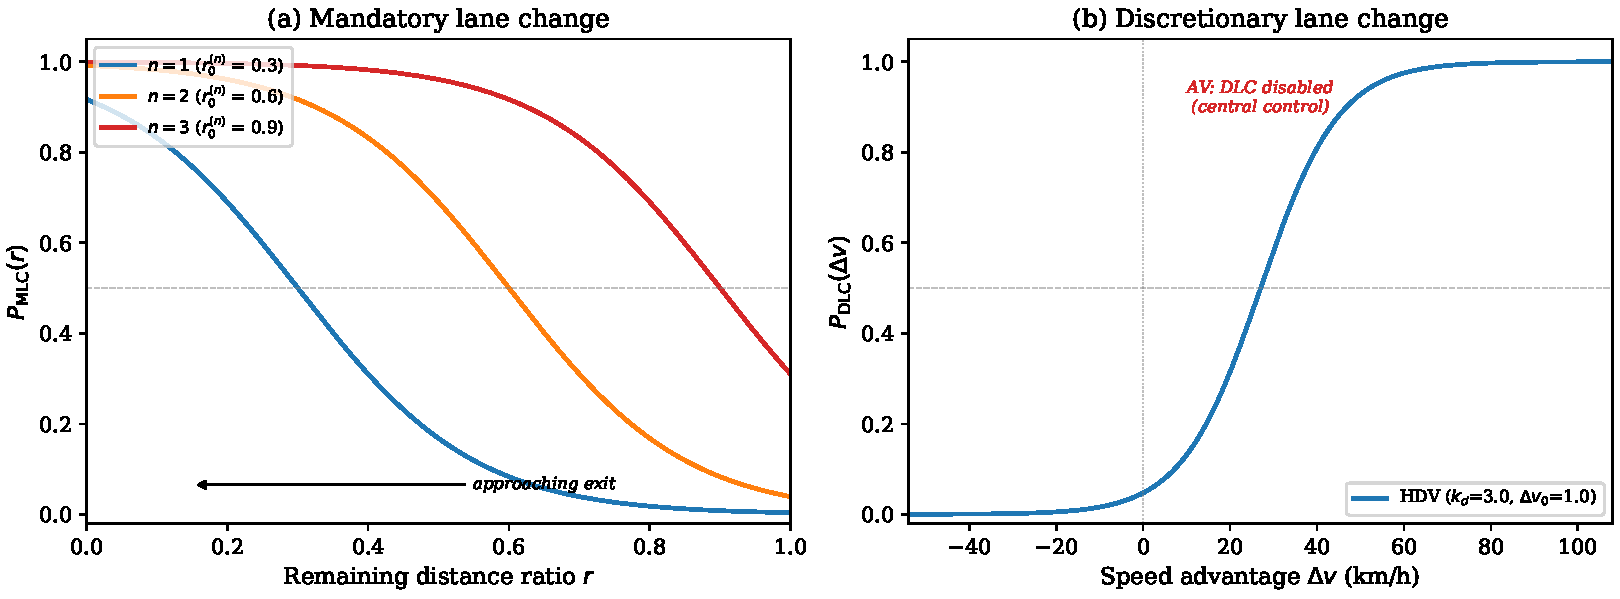
\includegraphics[width=\textwidth]{../figures/fig_lc_logistic.pdf}
    \caption{Lane-change logistic probabilities. (a)~MLC probability as a function of the remaining distance ratio $r$ for different numbers of required lane changes $n$. A single lane change ($n=1$) triggers action close to the exit, while $n=3$ induces merging much earlier. (b)~DLC probability as a function of the speed advantage $\Delta v$ for HDVs. Centrally controlled AVs do not perform discretionary lane changes.}
    \label{fig:lc_logistic}
\end{figure}

Figure~\ref{fig:lc_logistic}a illustrates how the logistic MLC model captures escalating urgency. A vehicle needing only one lane change can afford to wait until the exit is nearby ($r \approx 0.3$), whereas a vehicle requiring three lane changes begins maneuvering when roughly 90\% of its trip remains --- mirroring how drivers on unfamiliar freeways begin merging well in advance when they must cross several lanes. Figure~\ref{fig:lc_logistic}b shows the HDV discretionary lane-change probability: drivers require a speed advantage of roughly 27~km/h before the lane-change probability reaches 0.5, modeling the cautious ``wait until it's obviously worth it'' attitude of human drivers. AVs do not perform discretionary lane changes; under central control, lane changes are executed only when mandatory (blockage avoidance or destination approach), eliminating the merge turbulence that opportunistic lane-seeking creates in mixed traffic.

\paragraph{Lane-Change Safety Assessment.}
Before executing a lane change, the driver evaluates the safety of the target lane by checking gaps to the nearest leader and follower in that lane. Rather than using fixed safety gaps, the framework employs speed-dependent gaps based on the closing speed between the lane-changing vehicle and its potential neighbors:
\begin{align}
    g_{\text{front}}^{\text{req}} &= d + (g_{\text{front}}^{\max} - d) \cdot \frac{\max(0,\; v - v_L)}{v_{\max}} \label{eq:front_gap} \\
    g_{\text{rear}}^{\text{req}} &= d + (g_{\text{rear}}^{\max} - d) \cdot \frac{\max(0,\; v_F - v)}{v_{\max}} \label{eq:rear_gap}
\end{align}
where $v_L$ and $v_F$ are the speeds of the target-lane leader and follower, and $g_{\text{front}}^{\max}$, $g_{\text{rear}}^{\max}$ are the maximum safety gap parameters. When the closing speed is zero (same speed or diverging), the required gap reduces to the standstill spacing $d$; when the closing speed is maximal, the full safety gap is required. This formulation avoids both overly conservative gap acceptance (which traps vehicles behind blockages) and overly aggressive merging (which disrupts the target lane).

\paragraph{Blockage-Aware MLC Urgency.}
When a vehicle detects a blocked cell within its look-ahead distance, the number of required lane changes in Eq.~\eqref{eq:mlc_logistic} is inflated by two: $n_{\text{LC}} \leftarrow n_{\text{LC}} + 2$, reflecting that the vehicle must change lane to pass the blockage and then return. This inflation increases $P_{\text{MLC}}$ at greater distances from the blockage, inducing earlier lane changes at higher speeds where natural gaps are available, rather than forcing late merges at low speeds near the blockage.

\paragraph{Lane-Change Execution.}
When the driver process decides to change lanes, the movement process executes the lateral transition at the next cell boundary by requesting the corresponding cell in the target lane rather than the longitudinal successor in the current lane. \DIFaddbegin \DIFadd{One decision produces one lane change: the requested direction returns to forward as soon as the lateral move is granted, so crossing several lanes takes one decision per lane, each with its own gap check and its own cooldown. }\DIFaddend During the transition, the vehicle holds resources in both the origin and destination lanes (via delayed release of the origin-lane cell), preventing conflicts. Vehicles that have been waiting behind a blockage receive elevated priority for cell requests, proportional to their waiting time, ensuring that trapped vehicles are not indefinitely starved by through-traffic in adjacent lanes.


\subsection{Integrated Framework}
\label{sec:integrated}

The ODCA-DES framework integrates the above components through a dual control architecture that distinguishes between human-driven and autonomous vehicles.

\subsubsection{Decentralized Control: Human-Driven Vehicles}

Each HDV, upon entering the freeway, spawns two concurrent processes:

\begin{enumerate}
    \item The \textbf{movement process} executes the cell-by-cell request--wait--seize--delay--release cycle (Section~\ref{sec:movement}), using the current speed set by the driver process.

    \item The \textbf{driver process} re-evaluates speed and direction (Section~\ref{sec:driver}), updating the vehicle's behavioral state. Re-evaluations are triggered either by the expiration of a maximum action interval $\delta_{\text{eval}}$ or by wake-up callbacks from neighboring vehicles' movements, whichever occurs first.
\end{enumerate}

These two processes communicate through shared vehicle state: the driver process writes the desired speed and lane-change intention; the movement process reads these values at each cell transition.

\subsubsection{Centralized Control: Autonomous Vehicles}
\label{sec:av_controller}

AVs do not run individual driver processes. Instead, a \textbf{central AV controller}---a single SimPy process---evaluates speed and direction for all active AVs at a fixed update interval $\Delta t_{\text{ctrl}}$. At each controller cycle, the controller iterates over all active AVs and executes the same car-following logic used by HDVs, but with AV-specific parameters ($\tau_{\text{AV}}$, zero slowdown probability, tighter safety gaps). Crucially, AVs perform only mandatory lane changes (blockage avoidance, destination approach); discretionary lane changes are disabled. Under central coordination, speed-seeking lane changes are unnecessary---the controller optimizes longitudinal behavior directly---and their absence eliminates the merge turbulence that arises when individually optimizing vehicles compete for gaps in adjacent lanes.

This architecture reflects the connected nature of autonomous vehicles: rather than each AV independently perceiving and reacting to its local environment, a shared controller with access to all AV states coordinates their behavior. The movement process remains per-vehicle---each AV still independently acquires and releases cell resources through the request--wait--seize--delay--release protocol.

The centralized architecture offers two advantages:
\begin{itemize}
    \item \textbf{Computational efficiency.} A single controller process generating one SimPy event per update cycle replaces $N_{\text{AV}}$ independent processes, each generating their own events. This reduces context-switching overhead from $O(N_{\text{AV}})$ to $O(1)$ events per controller cycle.
    \item \textbf{Extensibility.} The controller provides a natural integration point for cooperative AV behaviors---platooning, coordinated merging, and anticipatory speed adjustments---that require global knowledge of the AV fleet state.
\end{itemize}

\subsubsection{Communication Through Shared State}

In both control modes, behavioral decisions (speed, direction) are communicated to the movement process through shared vehicle state variables. The decoupling ensures that:

\begin{itemize}
    \item A vehicle in free flow with no nearby interactions generates minimal events (one seize--release pair per cell, plus periodic driver or controller re-evaluations).
    \item A vehicle in congestion generates events driven by resource contention, with speed adjustments in response to changing gaps.
    \item The movement engine is agnostic to the control mode---it consumes the same state interface regardless of whether decisions originate from a per-vehicle driver process or the central controller.
\end{itemize}

Figure~\ref{fig:architecture} illustrates the overall architecture.

\begin{figure}[ht]
    \centering
    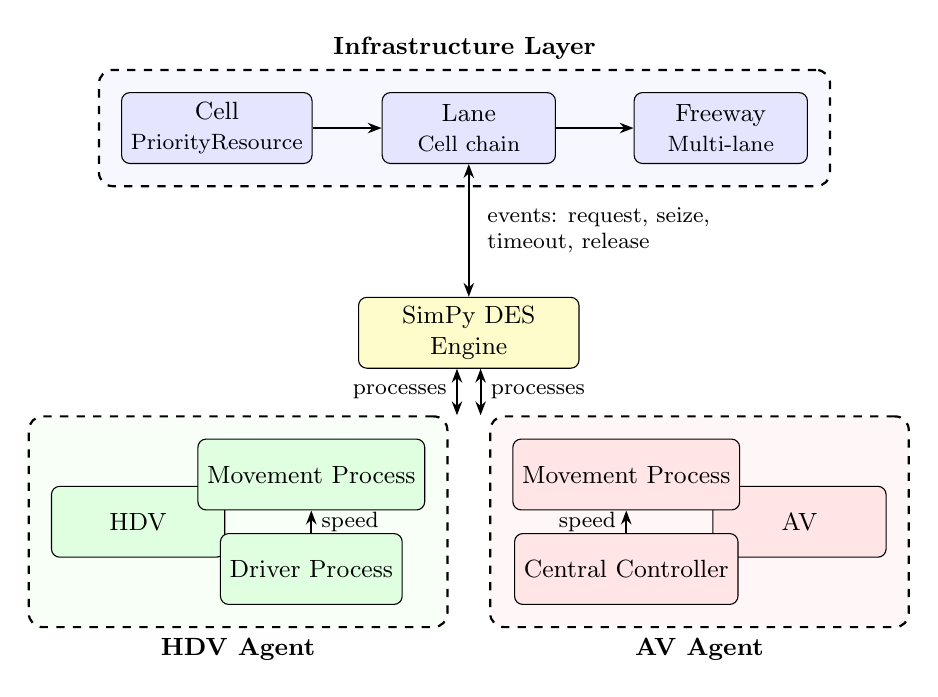
\begin{tikzpicture}[
        box/.style={draw, rounded corners=3pt, minimum width=2.2cm, minimum height=0.9cm,
                     align=center, font=\small},
        bigbox/.style={draw, rounded corners=5pt, inner sep=8pt, dashed, thick},
        arr/.style={-{Stealth[length=5pt]}, thick},
        darr/.style={{Stealth[length=5pt]}-{Stealth[length=5pt]}, thick},
    ]
    % Infrastructure layer — centered at origin
    \node[box, fill=blue!10] (lane) at (0,0) {Lane\\{\footnotesize Cell chain}};
    \node[box, fill=blue!10] (cell) at (-3.2,0) {Cell\\{\footnotesize PriorityResource}};
    \node[box, fill=blue!10] (freeway) at (3.2,0) {Freeway\\{\footnotesize Multi-lane}};
    \draw[arr] (cell) -- (lane);
    \draw[arr] (lane) -- (freeway);

    % DES Engine — centered below infrastructure
    \node[box, fill=yellow!20, minimum width=2.8cm] (engine) at (0,-2.6) {SimPy DES\\Engine};

    % HDV Agent — left side, two rows inside group
    \node[box, fill=green!12] (hdv) at (-4.2,-5.0) {HDV};
    \node[box, fill=green!12] (mvmt) at (-2.0,-4.4) {Movement Process};
    \node[box, fill=green!12] (driver) at (-2.0,-5.6) {Driver Process};
    \draw[arr] (driver) -- node[right, font=\footnotesize] {speed} (mvmt);

    % AV Agent — right side, two rows inside group
    \node[box, fill=red!10] (av) at (4.2,-5.0) {AV};
    \node[box, fill=red!10] (avmvmt) at (2.0,-4.4) {Movement Process};
    \node[box, fill=red!10] (ctrl) at (2.0,-5.6) {Central Controller};
    \draw[arr] (ctrl) -- node[left, font=\footnotesize] {speed} (avmvmt);

    % Grouping boxes
    \begin{scope}[on background layer]
        \node[bigbox, fill=blue!3, fit=(cell)(lane)(freeway),
              label={[font=\small\bfseries]above:Infrastructure Layer}] (infra) {};
        \node[bigbox, fill=green!3, fit=(hdv)(mvmt)(driver),
              label={[font=\small\bfseries]below:HDV Agent}] (hdvbox) {};
        \node[bigbox, fill=red!3, fit=(av)(avmvmt)(ctrl),
              label={[font=\small\bfseries]below:AV Agent}] (avbox) {};
    \end{scope}

    % Arrow — infrastructure to engine
    \draw[darr] (engine.north) -- node[right, font=\footnotesize, align=left, xshift=3pt]
        {events: request, seize,\\timeout, release} (lane.south);

    % Arrows — vehicle groups to engine
    \coordinate (eng_bl) at ($(engine.south) + (-0.15,0)$);
    \coordinate (eng_br) at ($(engine.south) + (0.15,0)$);
    \draw[darr] (eng_bl) -- node[left, font=\footnotesize] {processes} (eng_bl |- hdvbox.north);
    \draw[darr] (eng_br) -- node[right, font=\footnotesize] {processes} (eng_br |- avbox.north);
    \end{tikzpicture}
    \caption{ODCA-DES framework architecture. Infrastructure objects provide the spatial resource structure; the DES engine manages event scheduling and process synchronization. HDVs encapsulate concurrent movement and driver processes, while AVs delegate behavioral decisions to a central controller.}
    \label{fig:architecture}
\end{figure}


% ============================================================
\section{Analytical Properties}
\label{sec:analytical}
% ============================================================

This section establishes key analytical properties of the ODCA-DES framework, demonstrating its consistency with established traffic flow theory.

\subsection{Trajectory Function and Newell's Coordinates}
\label{sec:trajectory_function}

The simulation output is a collection of passage-time records $\Tarr(c, i)$ for each vehicle $i$ at each cell $c$. This is precisely the $T(x, n)$ coordinate system described by \citet{newell1993simplified}, where $x$ corresponds to the cell position $c \cdot \ell$ and $n$ corresponds to the vehicle index.

From the passage-time data, all standard traffic flow variables can be derived without spatial or temporal aggregation:

\begin{itemize}
    \item \textbf{Speed} at cell $c$ for vehicle $i$:
    \begin{equation}
        v_i(c) = \frac{\ell}{\Tarr(c+1, i) - \Tarr(c, i)}
        \label{eq:speed_from_T}
    \end{equation}
    Note that this is the travel speed (including any waiting time), not the running speed.

    \item \textbf{Headway} at cell $c$ between consecutive vehicles:
    \begin{equation}
        h(c) = \Tarr(c, i) - \Tarr(c, i-1)
        \label{eq:headway_from_T}
    \end{equation}

    \item \textbf{Flow} at cell $c$:
    \begin{equation}
        q(c) = \frac{1}{h(c)}
        \label{eq:flow_from_T}
    \end{equation}

    \item \textbf{Cumulative count} $N(t, x)$ can be constructed by counting arrivals at position $x$ up to time $t$, connecting to the LWR theory \citep{lighthill1955kinematic, richards1956shock} and its variational formulation \citep{daganzo2005variational}.
\end{itemize}

\subsection{Fundamental Diagram Derivation}
\label{sec:fd_derivation}

We derive the steady-state fundamental diagram (FD) implied by the ODCA-DES framework, showing that the resource-based movement protocol produces a triangular FD consistent with Newell's kinematic wave model.

\subsubsection{Free-Flow Regime}

In the absence of resource contention, each vehicle travels at its \DIFdelbegin \DIFdel{desired }\DIFdelend free-flow speed \DIFaddbegin \DIFadd{(Eq.~\ref{eq:free_flow_speed}). The derivation below treats a homogeneous stream on a uniform road, where every vehicle has the same maximum speed and every cell the same posted limit, so that $v_f^{(i)}(c)$ is one scalar }\DIFaddend $v_f$ \DIFaddbegin \DIFadd{for the whole segment}\DIFaddend . The travel time per cell is $\ell / v_f$, and consecutive cells are acquired without waiting. The density of a single-lane stream of vehicles all traveling at $v_f$ with headway $h$ is:
\begin{equation}
    k = \frac{1}{v_f \cdot h} = \frac{1}{v_f \cdot (\tau + \ell / v_f)} = \frac{1}{v_f \tau + \ell}
    \label{eq:density_freeflow}
\end{equation}
and the flow is:
\begin{equation}
    q = k \cdot v_f = \frac{v_f}{v_f \tau + \ell}
    \label{eq:flow_freeflow}
\end{equation}

For low densities where $h > \tau + \ell / v_f$ (i.e., inter-vehicle gaps exceed the minimum headway), vehicles are unconstrained and all travel at $v_f$. In this regime, flow increases linearly with density:
\begin{equation}
    q = k \cdot v_f, \qquad 0 \leq k \leq k_c
    \label{eq:fd_freeflow}
\end{equation}
where the critical density $k_c$ corresponds to the maximum flow:
\begin{equation}
    k_c = \frac{1}{v_f \tau + \ell}
    \label{eq:critical_density}
\end{equation}

\subsubsection{Congested Regime}

When a vehicle encounters an occupied cell, it waits until the predecessor releases it. In steady-state car following at speed $v < v_f$, the headway is $h = \tau + \ell / v$ (Eq.~\ref{eq:headway}), and the spacing (in cells) is:
\begin{equation}
    s = v \cdot h = v\tau + \ell
    \label{eq:spacing_congested}
\end{equation}

The density is $k = 1/s = 1/(v\tau + \ell)$, giving:
\begin{equation}
    v = \frac{1 - k\ell}{k\tau} = \frac{1}{k\tau} - \frac{\ell}{\tau}
    \label{eq:speed_density_congested}
\end{equation}

The flow in the congested regime is:
\begin{equation}
    q = k \cdot v = \frac{1}{\tau} - \frac{k\ell}{\tau} = \frac{1}{\tau}\left(1 - k\ell\right)
    \label{eq:flow_congested}
\end{equation}

This is a linear function of density with slope $-\ell/\tau$, which is precisely the backward wave speed $w$:
\begin{equation}
    w = -\frac{\ell}{\tau}
    \label{eq:wave_speed}
\end{equation}

The jam density (when $v = 0$) is:
\begin{equation}
    k_j = \frac{1}{\ell}
    \label{eq:jam_density}
\end{equation}
corresponding to one vehicle per cell with zero speed---exactly the physical constraint imposed by the single-occupancy cell resource.

\subsubsection{Capacity and Triangular FD}

The capacity (maximum flow) occurs at the critical density $k_c$, where the free-flow and congested branches meet:
\begin{equation}
    q_{\max} = \frac{v_f}{v_f \tau + \ell}
    \label{eq:capacity}
\end{equation}

The resulting fundamental diagram is triangular (Figure~\ref{fig:fd_theoretical}):
\begin{equation}
    q(k) = \begin{cases}
        k \cdot v_f & \text{if } k \leq k_c \\[4pt]
        \dfrac{1}{\tau}(1 - k\ell) & \text{if } k_c < k \leq k_j
    \end{cases}
    \label{eq:triangular_fd}
\end{equation}

This triangular FD---a two-regime piecewise-linear relationship first motivated by the empirical observations of \citet{greenshields1935study}---is identical to that derived from Newell's kinematic wave model \citep{newell1993simplified} and the Cell Transmission Model \citep{daganzo1994cell}. The key insight is that the two parameters controlling the FD shape---$v_f$ (free-flow speed) and $w = \ell/\tau$ (backward wave speed)---emerge directly from the ODCA-DES model parameters: the cell length $\ell$ and the delayed release time $\tau$. No additional calibration of the FD is needed; it is an inherent consequence of the resource protocol.

\subsubsection{Heterogeneous Traffic}

When multiple vehicle types share the same lane, each type contributes its own headway parameters ($\tau$, $d$). In a mixed AV/HDV stream, a follower behind a leader produces headway:
\begin{equation}
    h = \tau_{\text{leader}} + \frac{\ell}{v}
    \label{eq:mixed_headway}
\end{equation}
Note that the headway depends on the \emph{leader's} release delay $\tau_{\text{leader}}$, since it is the leader's delayed release that governs when the follower can acquire the cell. In a stream with AV fraction $\alpha$, the expected headway is:
\begin{equation}
    \bar{h}(v) = \left[\alpha \tau_{\text{AV}} + (1-\alpha)\tau_{\text{HDV}}\right] + \frac{\ell}{v}
    \label{eq:mixed_avg_headway}
\end{equation}
yielding a capacity that increases with AV penetration (since $\tau_{\text{AV}} < \tau_{\text{HDV}}$):
\begin{equation}
    q_{\max}(\alpha) = \frac{v_f}{v_f\left[\alpha \tau_{\text{AV}} + (1-\alpha)\tau_{\text{HDV}}\right] + \ell}
    \label{eq:mixed_capacity}
\end{equation}

This provides a closed-form expression for the capacity benefit of AV penetration under the ODCA-DES framework.


\subsection{Comparison with Synchronous Cellular Automata}
\label{sec:ca_comparison}

To clarify the distinctions between the ODCA-DES framework and classical CA models, we present a detailed comparison along three dimensions: speed representation, update synchronization, and conflict resolution. We then illustrate these differences through a worked example.

\DIFaddbegin \DIFadd{Figure~\ref{fig:paradigm} shows what the two paradigms represent differently, on the same eight vehicles on the same road, both models deterministic so that only the representation differs. The platoon starts at rest at the free-flow spacing, accelerates, meets a posted zone of 21 cells where the limit is 2\,cells/s (54\,km/h), and accelerates again once it is past; every follower repeats the leader's move a little later and a little further upstream, which is the shape any car-following model must produce. In panel~(a) the NaSch platoon exists only at whole seconds and only at whole cells: the lead vehicle is at cell~64 at $t = 2$\,s and at cell~67 at $t = 3$\,s, and the model says nothing about where it was in between, because there is no in between. In panel~(b) the same platoon under ODCA-DES has a mark wherever a vehicle entered a cell, and those instants are whatever the crossing times make them: of the 1}{\DIFadd{,}}\DIFadd{328 cell entries in the window, 14 fall on a whole second. The space axis is identical in both, which is the point of keeping the cell: ODCA-DES relaxes the time axis and the speed value, not the spatial discretisation that makes a CA cheap. Panel~(c) follows the last vehicle, the one the zone holds longest. The NaSch speed climbs through the integers 0, 1, 2, 3, 4, 5 and can hold no value between them, so both the approach to the zone and the departure from it are whole-cell steps; the ODCA-DES speed takes 19 distinct values between 1.86 and 5.20\,cells/s, slides down through them as the gap to the vehicle ahead closes, holds the posted 2.00\,cells/s exactly through all 21 cells of the zone, and returns to the 5.2\,cells/s (140\,km/h) of Table~\ref{tab:vehicle_params}, a speed an integer-cell-per-second model cannot express at all: its nearest representable free-flow speeds are 5\,cells/s (135\,km/h) and 6\,cells/s (162\,km/h). The return is a single step rather than a ramp, and the asymmetry is worth naming: the approach to the zone is gradual because the vehicle ahead constrains it through Eq.~\ref{eq:newell_cf}, while nothing constrains a vehicle whose road is clear. Both models are first order, with speed a function of spacing and no vehicle-dynamics layer, so neither bounds acceleration. Bounding it on its own would not refine that: the same spacing rule already prescribes decelerations of up to 1.5\,cells/s$^2$ (11.3\,m/s$^2$) where a free-flowing vehicle meets a standing queue nine cells ahead, so a vehicle held to a plausible acceleration limit but not a braking one would not describe a car. A model with acceleration on both branches means a second-order car-following law in place of Eq.~\ref{eq:newell_cf}, which is outside the scope of this paper.
}

\begin{figure}[htbp]
    \centering
    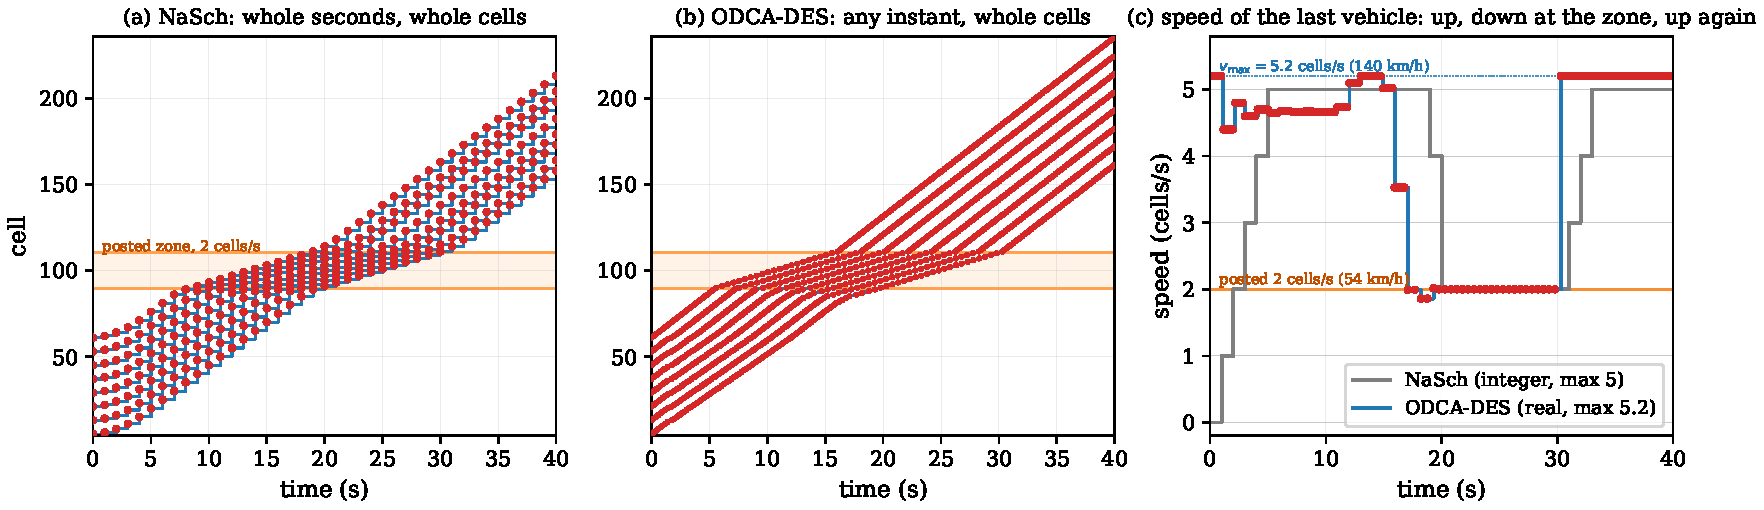
\includegraphics[width=\textwidth]{../figures/fig_paradigm_comparison.pdf}
    \caption{\DIFaddFL{What the two paradigms represent, on the same eight vehicles through the same posted speed-limit zone (shaded, 21 cells at 2\,cells/s), both models deterministic (no random slowdown, no driver heterogeneity). The platoon accelerates, slows at the zone and accelerates again, and each follower repeats the move behind the one ahead. (a)~NaSch: a red mark is a position, and there is one per vehicle per whole second, each a whole number of cells ahead of the last. (b)~ODCA-DES: a red mark is a cell entry, and it occurs at whatever instant the crossing takes; 14 of the 1}{\DIFaddFL{,}}\DIFaddFL{328 entries shown fall on a whole second. The cell axis is the same in both. (c)~The speed of the last vehicle: NaSch steps through the integers 0 to 5\,cells/s, while ODCA-DES passes through 19 distinct values between 1.86 and 5.20, holds the posted 2.00 exactly, and returns to the 5.2\,cells/s that the integer model has no way to name. Produced by }\texttt{\DIFaddFL{code/plot\_paradigm\_comparison.py}}\DIFaddFL{.}}
    \label{fig:paradigm}
\end{figure}

\DIFaddend \subsubsection{Speed Representation}

In the NaSch model \citep{nagel1992cellular}, vehicle speed is an integer $v \in \{0, 1, \ldots, v_{\max}\}$ representing cells per timestep. This discretization produces a stepped fundamental diagram: flow can only take values corresponding to integer speed--density combinations, creating artifacts particularly at low densities where vehicles oscillate between adjacent integer speeds rather than settling at a continuous equilibrium.

In ODCA-DES, speed is continuous-valued, $v \in [0, v_{\max}]$. The travel time per cell is $\ell/v$, which takes any positive real value. The DES event scheduler handles these continuous inter-event times exactly, producing smooth speed distributions and a continuous fundamental diagram without discretization artifacts.

\subsubsection{Update Synchronization}

The NaSch model updates all vehicles simultaneously in four sequential sub-steps (acceleration, deceleration, randomization, movement) applied globally at each timestep. This parallel update introduces two artifacts:
\begin{enumerate}
    \item \textbf{Symmetry in interactions:} Two vehicles approaching each other effectively ``see'' each other's previous-timestep positions, not their current positions. This creates artificial simultaneity in conflict resolution.
    \item \textbf{Uniform temporal resolution:} All vehicles, regardless of their local traffic context, are updated at the same frequency. A vehicle in free flow with no nearby neighbors receives the same computational attention as a vehicle in a dense platoon.
\end{enumerate}

In ODCA-DES, each vehicle evolves on its own event timeline. A vehicle's next event is scheduled based on its current speed and resource availability, not a global clock. Two vehicles interact only when they compete for the same cell resource, and the interaction is resolved in real time through the DES event calendar. This naturally concentrates computation where interactions occur.

\subsubsection{Conflict Resolution}

In the NaSch model, conflicts are resolved by explicit rules. The deceleration step checks whether the gap to the leader (measured in cells) is less than the current speed; if so, the speed is reduced to match the gap. This rule-based approach requires careful ordering of sub-steps to avoid inconsistencies.

In ODCA-DES, conflicts are resolved by the resource contention mechanism. A vehicle requesting an occupied cell simply waits---its process is suspended by the DES scheduler until the resource becomes available. No explicit gap-checking is performed. The deceleration effect emerges because the waiting time increases the effective travel time between cells, reducing the measured travel speed. This mechanism is:
\begin{itemize}
    \item \textbf{Deadlock-free:} Vehicles move in one direction, so circular resource dependencies cannot arise.
    \item \textbf{Order-preserving:} The priority resource ensures first-come-first-served access, maintaining vehicle ordering within a lane.
    \item \textbf{Physically consistent:} The waiting time exactly corresponds to the time the predecessor physically occupies the cell (via the delayed release), so the resulting headway is consistent with the car-following model.
\end{itemize}

\subsubsection{Illustrative Example}

Consider three vehicles ($A$, $B$, $C$) on a single-lane road with cells indexed $1, 2, \ldots, 10$. At time $t=0$: vehicle $A$ is at cell~8 with speed $v_A = 2\;\text{cells/s}$, vehicle $B$ is at cell~5 with speed $v_B = 3\;\text{cells/s}$, and vehicle $C$ is at cell~1 with speed $v_C = 3\;\text{cells/s}$. Parameters: $\tau = 1\;\text{s}$, $\ell = 1\;\text{cell}$.

\paragraph{NaSch evolution ($\Delta t = 1\;\text{s}$, $v_{\max} = 3$).}
At each timestep, all vehicles simultaneously execute: (1) accelerate by~1 (up to $v_{\max}$), (2) decelerate if gap $<$ speed, (3) randomize, (4) move. Table~\ref{tab:nasch_example} traces the resulting state evolution.

\begin{table}[ht]
\centering
\caption{NaSch synchronous update for three vehicles. Speeds are integers; all updates occur simultaneously at each timestep. $^*$Deceleration applied due to gap constraint.}
\label{tab:nasch_example}
\begin{tabular}{@{}ccccccc@{}}
\toprule
$t$ & \multicolumn{2}{c}{Vehicle $A$} & \multicolumn{2}{c}{Vehicle $B$} & \multicolumn{2}{c}{Vehicle $C$} \\
\cmidrule(lr){2-3} \cmidrule(lr){4-5} \cmidrule(lr){6-7}
 & cell & $v$ & cell & $v$ & cell & $v$ \\
\midrule
0 & 8 & 2 & 5 & 3 & 1 & 3 \\
1 & 10 & 3 & 8 & 3 & 4 & 3 \\
2 & exit & -- & 11$^*$ & 2$^*$ & 7 & 3 \\
3 & -- & -- & exit & -- & 9 & 2$^*$ \\
\bottomrule
\end{tabular}
\end{table}

Note that at $t=1$, vehicle $B$ reaches cell~8 simultaneously as vehicle $A$ departs---the synchronous update allows this because both see each other's $t=0$ state. Speed adjustments are abrupt (integer steps), and the gap-checking rule must be carefully ordered to avoid collisions.

\paragraph{ODCA-DES evolution.}
Each vehicle schedules events independently. Vehicle $A$ at cell~8 with $v_A = 2$ schedules: request cell~9 at $t = 0.5$\,s. Vehicle $B$ at cell~5 with $v_B = 3$ schedules: request cell~6 at $t = 0.33$\,s. Events are processed in chronological order, as shown in Table~\ref{tab:odca_example}.

\begin{table}[ht]
\centering
\caption{ODCA-DES event sequence for three vehicles. Times are continuous; events are processed in chronological order. Each vehicle advances independently until resource contention occurs.}
\label{tab:odca_example}
\begin{tabular}{@{}clll@{}}
\toprule
Time (s) & Event & Vehicle & Notes \\
\midrule
0.000 & Initialize & $A,B,C$ & $A$@8, $B$@5, $C$@1 \\
0.333 & Acquire cell 6 & $B$ & Free; seize immediately \\
0.333 & Acquire cell 2 & $C$ & Free; seize immediately \\
0.500 & Acquire cell 9 & $A$ & Free; seize immediately \\
0.667 & Acquire cell 7 & $B$ & Free \\
0.667 & Acquire cell 3 & $C$ & Free \\
1.000 & Release cell 8 & $A$ & Delayed release: $\Tacq(9) + \tau = 0.5 + 1.0$ \\
1.000 & Acquire cell 10 & $A$ & Free \\
1.000 & Acquire cell 8 & $B$ & \textbf{Wait}: $A$ holds cell 8 until $t=1.5$ \\
1.000 & Acquire cell 4 & $C$ & Free \\
1.333 & Acquire cell 5 & $C$ & Released by $B$ at $t = 1.333$ \\
1.500 & Release cell 8 & $A$ & $\Tacq(9,A) + \tau = 0.5 + 1.0 = 1.5$ \\
1.500 & Acquire cell 8 & $B$ & Resource freed; $B$ seizes \\
\bottomrule
\end{tabular}
\end{table}

Several key differences are visible:
\begin{enumerate}
    \item \textbf{Continuous timing:} Events occur at $t = 0.333, 0.500, 0.667, \ldots$ rather than at integer timesteps, reflecting the continuous speeds.
    \item \textbf{Asynchronous interaction:} Vehicle $C$ is completely independent of $A$ and $B$ throughout; it generates events on its own timeline without waiting for a global clock tick.
    \item \textbf{Resource-mediated conflict:} Vehicle $B$ does not ``check its gap'' to $A$. Instead, it requests cell~8, finds it occupied, and waits. The delay emerges from $A$'s release schedule, not from an explicit deceleration rule.
    \item \textbf{Headway emergence:} $B$ acquires cell~8 at $t = 1.5$, exactly $\tau = 1.0$\,s after $A$ acquired cell~9 at $t = 0.5$. The headway $h = \tau + \ell/v$ is produced by the resource protocol without any headway-enforcement rule.
\end{enumerate}

Table~\ref{tab:comparison_summary} summarizes the structural differences between the two frameworks.

\begin{table}[ht]
\centering
\caption{Structural comparison of the NaSch CA model and the ODCA-DES framework.}
\label{tab:comparison_summary}
\begin{tabular}{@{}lll@{}}
\toprule
Dimension & NaSch CA & ODCA-DES \\
\midrule
Speed domain & Integer $\{0,1,\ldots,v_{\max}\}$ & Continuous $[0, v_{\max}]$ \\
Time advancement & Fixed $\Delta t$ (synchronous) & Event-to-event (asynchronous) \\
Update order & Parallel (all vehicles) & Per-vehicle (own timeline) \\
Conflict resolution & Rule-based gap check & Resource contention (wait) \\
Headway control & Explicit deceleration rule & Emerges from delayed release \\
FD shape & Stepped (integer artifacts) & Smooth (triangular) \\
Coordinate system & $X(t,n)$ via position update & $T(x,n)$ via passage times \\
Heterogeneity & Difficult (same update cycle) & Natural (per-vehicle parameters) \\
\bottomrule
\end{tabular}
\end{table}


% ============================================================
\section{Computational Experiments}
\label{sec:experiments}
% ============================================================

This section presents computational experiments designed to validate the analytical properties derived in Section~\ref{sec:analytical} and demonstrate the framework's capabilities for modeling heterogeneous multi-lane freeway traffic. All experiments are implemented using the ODCA-DES framework built on SimPy \citep{simpy2023} in Python~3.10, executed on a Linux workstation with an Intel Core i7-1255U (12 cores) and 32\,GB RAM. Wall-clock times reported throughout this section are measured as elapsed real time for the complete simulation run (excluding file I/O). Random number generation uses NumPy's \texttt{SeedSequence} to produce independent per-source streams.

\subsection{Experimental Setup}
\label{sec:exp_setup}

\subsubsection{Network Configuration}

The test network is a four-lane unidirectional freeway segment of length $L = 6\;\text{km}$ (800 cells at $\ell = 7.5\;\text{m}$ per cell). Lanes are indexed from 1 (rightmost) to 4 (leftmost). The network includes:
\begin{itemize}
    \item \textbf{On-ramp 1:} at cell 100 (750\,m from the start), merging into lane~1.
    \item \textbf{On-ramp 2:} at cell 400 (3.0\,km from the start), merging into lane~1.
    \item \textbf{Off-ramp 1:} at cell 300 (2.25\,km), exiting from lane~1.
    \item \textbf{Off-ramp 2:} at cell 550 (4.125\,km), exiting from lane~1.
    \item \textbf{Off-ramp 3:} at cell 750 (5.625\,km), exiting from lane~1.
\end{itemize}

The mainline entry (cell~1) serves as the primary source, with vehicles distributed across all four lanes according to an initial lane-assignment probability proportional to lane capacity. Figure~\ref{fig:network} illustrates the network geometry.

\begin{figure}[ht]
    \centering
    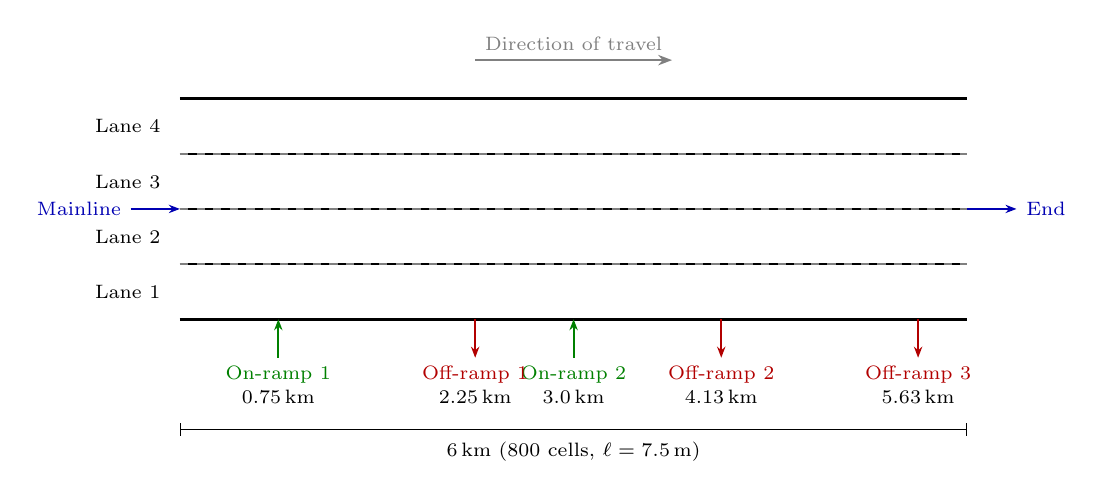
\begin{tikzpicture}[
        x=1.25cm, y=0.7cm,
        ramp/.style={-{Stealth[length=4pt]}, thick},
        lbl/.style={font=\scriptsize},
    ]
    % Freeway lanes — 5 lines creating 4 lane bands
    \foreach \y in {0,1,2,3,4} {
        \draw[thick] (0,\y) -- (8,\y);
    }
    % Dashed lane dividers (inner boundaries)
    \foreach \y in {1,2,3} {
        \draw[thick, dashed, gray] (0,\y) -- (8,\y);
    }
    % Solid edge lines (top and bottom)
    \draw[very thick] (0,0) -- (8,0);
    \draw[very thick] (0,4) -- (8,4);

    % Lane labels (left side, centered in each band)
    \node[lbl, anchor=east] at (-0.1,0.5) {Lane 1};
    \node[lbl, anchor=east] at (-0.1,1.5) {Lane 2};
    \node[lbl, anchor=east] at (-0.1,2.5) {Lane 3};
    \node[lbl, anchor=east] at (-0.1,3.5) {Lane 4};

    % Mainline entry
    \draw[ramp, blue!70!black] (-0.5,2) -- (0,2);
    \node[lbl, blue!70!black, anchor=east] at (-0.5,2) {Mainline};
    % Exit
    \draw[ramp, blue!70!black] (8,2) -- (8.5,2);
    \node[lbl, blue!70!black, anchor=west] at (8.5,2) {End};

    % On-ramps (arrows pointing up into lane 1, labels below)
    % On-ramp 1 at 0.75 km  -> x = 0.75/6*8 = 1.0
    \draw[ramp, green!50!black] (1.0,-0.7) -- (1.0,0);
    \node[lbl, green!50!black] at (1.0,-1.0) {On-ramp 1};
    \node[lbl] at (1.0,-1.4) {\scriptsize 0.75\,km};

    % On-ramp 2 at 3.0 km  -> x = 3.0/6*8 = 4.0
    \draw[ramp, green!50!black] (4.0,-0.7) -- (4.0,0);
    \node[lbl, green!50!black] at (4.0,-1.0) {On-ramp 2};
    \node[lbl] at (4.0,-1.4) {\scriptsize 3.0\,km};

    % Off-ramps (arrows pointing down from lane 1, labels below)
    % Off-ramp 1 at 2.25 km -> x = 2.25/6*8 = 3.0
    \draw[ramp, red!70!black] (3.0,0) -- (3.0,-0.7);
    \node[lbl, red!70!black] at (3.0,-1.0) {Off-ramp 1};
    \node[lbl] at (3.0,-1.4) {\scriptsize 2.25\,km};

    % Off-ramp 2 at 4.125 km -> x = 4.125/6*8 = 5.5
    \draw[ramp, red!70!black] (5.5,0) -- (5.5,-0.7);
    \node[lbl, red!70!black] at (5.5,-1.0) {Off-ramp 2};
    \node[lbl] at (5.5,-1.4) {\scriptsize 4.13\,km};

    % Off-ramp 3 at 5.625 km -> x = 5.625/6*8 = 7.5
    \draw[ramp, red!70!black] (7.5,0) -- (7.5,-0.7);
    \node[lbl, red!70!black] at (7.5,-1.0) {Off-ramp 3};
    \node[lbl] at (7.5,-1.4) {\scriptsize 5.63\,km};

    % Distance scale
    \draw[|-|, thin] (0,-2.0) -- (8,-2.0);
    \node[lbl] at (4,-2.4) {6\,km (800 cells, $\ell = 7.5$\,m)};

    % Direction arrow
    \draw[-{Stealth[length=5pt]}, thick, gray] (3,4.7) -- (5,4.7);
    \node[lbl, gray, above] at (4,4.7) {Direction of travel};

    \end{tikzpicture}
    \caption{Test network geometry: 4-lane unidirectional freeway segment (6\,km, 800 cells at $\ell = 7.5$\,m). On-ramps merge into lane~1 (rightmost); off-ramps exit from lane~1. Mainline demand enters at \DIFaddbeginFL \DIFaddFL{the first }\DIFaddendFL cell \DIFdelbeginFL \DIFdelFL{~1 across all four lanes}\DIFdelendFL \DIFaddbeginFL \DIFaddFL{of each lane}\DIFaddendFL ; \DIFdelbeginFL \DIFdelFL{vehicles destined }\DIFdelendFL \DIFaddbeginFL \DIFaddFL{traffic bound }\DIFaddendFL for the segment end \DIFaddbeginFL \DIFaddFL{is spread over the four lane ends }\DIFaddendFL (cell~800)\DIFdelbeginFL \DIFdelFL{exit from their current lane}\DIFdelendFL \DIFaddbeginFL \DIFaddFL{, so it crosses lanes in both directions}\DIFaddendFL .}
    \label{fig:network}
\end{figure}

\subsubsection{Vehicle Parameters}

Two vehicle types are modeled: human-driven vehicles (HDVs) and autonomous vehicles (AVs). Table~\ref{tab:vehicle_params} summarizes the behavioral parameters for each type.

\begin{table}[ht]
\centering
\caption{Vehicle behavioral parameters used in the computational experiments.}
\label{tab:vehicle_params}
\begin{tabular}{@{}llcc@{}}
\toprule
Parameter & Symbol & HDV & AV \\
\midrule
Reaction time / release delay & $\tau$ & 1.5\,s & 0.5\,s \\
Standstill spacing & $d$ & 1 cell (7.5\,m) & 1 cell (7.5\,m) \\
Maximum speed & $v_{\max}$ & 5.2\,cells/s (140\,km/h) & 5.2\,cells/s (140\,km/h) \\
Random slowdown probability & $p$ & 0.15 & 0.0 \\
Slowdown decrement & $\delta v$ & 0.5\,cells/s & -- \\
MLC steepness & $k$ & 8.0 & 8.0 \\
MLC midpoint & $r_0$ & 0.3 & 0.3 \\
DLC sensitivity & $k_d$ & 3.0 & -- (disabled) \\
DLC speed threshold & $\Delta v_0$ & 1.0\,cells/s & -- (disabled) \\
DLC cooldown & -- & 10.0\,s & -- (disabled) \\
\DIFdelbeginFL \DIFdelFL{Perception delay }\DIFdelendFL \DIFaddbeginFL \DIFaddFL{MLC exposure reference }& \DIFaddFL{$\ell_{\text{ref}}$ }& \DIFaddFL{5.2\,cells (1\,s at $v_{\max}$) }& \DIFaddFL{5.2\,cells (1\,s at $v_{\max}$) }\\
\DIFaddFL{DLC exposure reference }& \DIFaddFL{-- }& \DIFaddFL{1.0\,s }\DIFaddendFL & -- \DIFaddbeginFL \DIFaddFL{(disabled) }\\
\DIFaddFL{Action interval (max.\ re-evaluation gap) }& \DIFaddFL{$\delta_{\text{eval}}$ }\DIFaddendFL & 1.0\,s & 0.1\,s \DIFaddbeginFL \DIFaddFL{(controller cycle) }\DIFaddendFL \\
Front safety gap & $g_{\text{front}}^{\max}$ & 2.0\,cells & 1.0\,cell \\
Rear safety gap & $g_{\text{rear}}^{\max}$ & 2.0\,cells & 1.0\,cell \\
\midrule
\multicolumn{4}{@{}l}{\emph{Per-driver heterogeneity (HDV only)}} \\
$\tau$ std.\ dev. & $\sigma_\tau$ & 0.3\,s & 0 (deterministic) \\
Action interval std.\ dev. & $\sigma_{\delta}$ & 0.2\,s & 0 (deterministic) \\
Slowdown prob.\ std.\ dev. & $\sigma_p$ & 0.05 & 0 (deterministic) \\
\bottomrule
\end{tabular}
\end{table}

The primary distinction is the reaction time: $\tau_{\text{HDV}} = 1.5$\,s vs.\ $\tau_{\text{AV}} = 0.5$\,s. This directly controls headway (Eq.~\ref{eq:headway}) and, consequently, lane capacity (Eq.~\ref{eq:capacity}). HDVs additionally experience random slowdowns ($p = 0.15$), introducing stochastic speed fluctuations absent in AVs.

To capture the heterogeneity of real driver populations, each HDV is assigned individual behavioral parameters at creation time by sampling from distributions centered on the mean values in Table~\ref{tab:vehicle_params}:
\begin{itemize}
    \item Reaction time: $\tau_i \sim \text{LogNormal}(\mu_\tau, \sigma_\tau)$, clipped to $[0.5, 3.0]$\,s.
    \item Action interval: $\delta_i \sim \text{LogNormal}(\mu_\delta, \sigma_\delta)$, clipped to $[0.3, 3.0]$\,s.
    \item Slowdown probability: $p_i \sim \mathcal{N}(\bar{p}, \sigma_p)$, clipped to $[0, 1]$.
\end{itemize}
The LogNormal distribution is chosen for $\tau$ and $\delta$ because both quantities are strictly positive and right-skewed in empirical observations. AVs use deterministic parameters (zero standard deviation), reflecting the consistency of automated control systems. This per-driver heterogeneity introduces capacity scatter in the fundamental diagram (Section~\ref{sec:exp_fd}) and more realistic platoon dynamics compared to homogeneous-driver models.

\subsubsection{Demand and Scenarios}
\DIFaddbegin \label{sec:demand}
\DIFaddend 

The simulation duration is $T_{\text{sim}} = 3600$\,s (1 hour). \DIFdelbegin \DIFdel{Mainline demand is set at 6000\,}\DIFdelend \DIFaddbegin \DIFadd{Origins and destinations are named places on the network: four mainline entries (one per lane, cell~0), two on-ramps (lane~1 at cells~100 and~400), three off-ramps (lane~1 at cells~300, 550 and~750) and one exit per lane at the segment end (cell~800). Demand is given as a flow in }\DIFaddend veh/h \DIFdelbegin \DIFdel{(1500}\DIFdelend \DIFaddbegin \DIFadd{for each origin--destination pair, and one generator per pair releases vehicles into its origin cell; a pair whose origin cell is occupied queues, so the road itself limits what enters.
}

\DIFadd{Mainline demand is 6}{\DIFadd{,}}\DIFadd{000}\DIFaddend \,veh/h \DIFdelbegin \DIFdel{/lane) , with on-ramps each contributing }\DIFdelend \DIFaddbegin \DIFadd{(1}{\DIFadd{,}}\DIFadd{500 per lane) and each on-ramp contributes }\DIFaddend 500\,veh/h. \DIFdelbegin \DIFdel{Vehicle destinations are assigned from per-lane origin--destination distributions that reflect realistic }\DIFdelend \DIFaddbegin \DIFadd{The split over destinations reflects }\DIFaddend lane-use patterns: \DIFdelbegin \DIFdel{inner lanes (lanes ~1--2) carry higher fractions of off-ramp-bound trafficrequiring mandatory lane changes, while outer lanes (lanes~3--4) are predominantly through-traffic destined for the segment end (cell~800). For example, lane}\DIFdelend \DIFaddbegin \DIFadd{the rightmost lanes carry most of the off-ramp traffic, the leftmost lanes mostly through traffic. Lane}\DIFaddend ~1 \DIFdelbegin \DIFdel{assigns }\DIFdelend \DIFaddbegin \DIFadd{sends }\DIFaddend 20\% of \DIFaddbegin \DIFadd{its }\DIFaddend vehicles to off-ramp~1, 25\% to off-ramp~2 \DIFdelbegin \DIFdel{, }\DIFdelend \DIFaddbegin \DIFadd{and }\DIFaddend 15\% to off-ramp~3, \DIFdelbegin \DIFdel{and }\DIFdelend \DIFaddbegin \DIFadd{keeping }\DIFaddend 40\% \DIFdelbegin \DIFdel{to the segment end}\DIFdelend \DIFaddbegin \DIFadd{through}\DIFaddend ; lane~4 \DIFdelbegin \DIFdel{assigns only }\DIFdelend \DIFaddbegin \DIFadd{sends }\DIFaddend 2\%, 5\% \DIFdelbegin \DIFdel{, }\DIFdelend and 3\% to the three off-ramps \DIFdelbegin \DIFdel{respectively, with }\DIFdelend \DIFaddbegin \DIFadd{and keeps }\DIFaddend 90\% \DIFdelbegin \DIFdel{through-traffic}\DIFdelend \DIFaddbegin \DIFadd{through}\DIFaddend . On-ramp~1 \DIFdelbegin \DIFdel{vehicles are split among }\DIFdelend \DIFaddbegin \DIFadd{splits between }\DIFaddend off-ramp~2 (50\%), off-ramp~3 (20\%) \DIFdelbegin \DIFdel{, }\DIFdelend and the segment end (30\%); on-ramp~2 \DIFdelbegin \DIFdel{vehicles go to }\DIFdelend \DIFaddbegin \DIFadd{between }\DIFaddend off-ramp~3 (30\%) \DIFdelbegin \DIFdel{or }\DIFdelend \DIFaddbegin \DIFadd{and }\DIFaddend the segment end (70\%). \DIFdelbegin \DIFdel{Vehicles with }\DIFdelend \DIFaddbegin \DIFadd{Through traffic is spread evenly over the four lane ends, so a share of every origin has to cross lanes in each direction rather than drive straight to the end of its entry lane. A vehicle bound for an }\DIFaddend off-ramp \DIFdelbegin \DIFdel{destinations must merge to }\DIFdelend \DIFaddbegin \DIFadd{must be in }\DIFaddend lane~1 \DIFdelbegin \DIFdel{, while segment-end vehicles exitfrom their current lane}\DIFdelend \DIFaddbegin \DIFadd{when it gets there; a vehicle bound for the end of lane~$j$ must be in lane~$j$. A vehicle that reaches the last cell in the wrong lane still leaves the network there, and the run records it as a missed exit.
}

\DIFadd{Endpoints are cells like any other, which is what lets a scenario throttle them: an origin or destination cell with its own speed limit caps the flow through it at $3600 / (\tau + \ell/v)$\,veh/h, an artificial bottleneck at a ramp or at the end of the segment. In the experiments reported here every endpoint is transparent (no speed limit, no time spent), so the network is the one described above. Capacity reductions inside the segment are modelled instead as }\emph{\DIFadd{incidents}}\DIFadd{: a set of cells is closed or slowed for a stated interval and then restored, which is how the lane-drop of Section~\ref{sec:exp_incident} is created}\DIFaddend .

Four scenarios, summarized in Table~\ref{tab:scenarios}, are evaluated to isolate the effects of AV penetration:

\begin{table}[ht]
\centering
\caption{Experimental scenarios varying AV penetration rate.}
\label{tab:scenarios}
\begin{tabular}{@{}clc@{}}
\toprule
Scenario & Description & AV Penetration ($\alpha$) \\
\midrule
S1 & Baseline (all HDV) & 0\% \\
S2 & Low AV penetration & 30\% \\
S3 & Moderate AV penetration & 50\% \\
S4 & High AV penetration & 70\% \\
\bottomrule
\end{tabular}
\end{table}

Each scenario is run with 20 independent replications (seeds 1--20) to account for stochastic variability in vehicle generation, type assignment, and HDV random slowdowns. All reported metrics are sample means with 95\% confidence intervals.

\DIFaddbegin \subsubsection{\DIFadd{Implementation and Hardware}}

\DIFadd{The framework is implemented in Python (3.13) on SimPy (4.1), with one process per vehicle, one per human driver and one for the AV controller; random numbers come from one NumPy }\texttt{\DIFadd{SeedSequence}} \DIFadd{stream per source of randomness, so a run is reproducible from its seed alone. Every run is single-threaded. The replications reported below were executed in parallel on a 12-core Intel Core i7-1255U, but every wall-clock figure quoted in Section~\ref{sec:exp_performance_new} comes from a run made alone on the same machine, since a timing measured next to eleven other simulations measures the machine, not the model.
}


\DIFaddend \subsection{Fundamental Diagram Validation}
\label{sec:exp_fd}

\subsubsection{Single-Lane Homogeneous Traffic}

To validate the theoretical FD derived in Section~\ref{sec:fd_derivation}, we simulate a single-lane closed segment (400 cells, no ramps) initialized at various densities ranging from $k = 0.01$ to $0.80$\,veh/cell. Vehicles are placed uniformly across the segment with an inflow process that replaces exiting vehicles to maintain the target density. Each configuration runs for 1200\,s with a 200\,s warm-up period. Flow--density pairs are computed using Edie's generalized definitions \citep{edie1963discussion} over a measurement region (cells 100--300) with 20-second aggregation windows:
\begin{equation}
    q = \frac{D}{A}, \qquad k = \frac{W}{A}
    \label{eq:fd_measurement}
\end{equation}
where $D$ is the total distance traveled by all vehicles within the space-time region of area $A = \Delta x \cdot \Delta T$, and $W$ is the total time spent by all vehicles within the region. This density-initialization approach produces a complete fundamental diagram spanning free-flow through jam density, and Edie's definitions ensure consistency between flow, density, and speed measurements.

The theoretical capacity for these parameters is:
\begin{equation}
    q_{\max} = \frac{5.2}{5.2 \times 1.5 + 1.0} = \frac{5.2}{8.8} \approx 0.591\;\text{veh/cell/s} = 2127\;\text{veh/h}
\end{equation}
and the backward wave speed is $w = \ell/\tau = 1.0/1.5 = 0.667$\,cells/s $= 18$\,km/h, consistent with empirically observed congestion wave speeds \citep{cassidy1998bivariate}.

\DIFaddbegin \DIFadd{Two measurements are worth separating here. On a ring road, where no vehicle enters or leaves, the simulated stream reaches 1}{\DIFadd{,}}\DIFadd{948\,veh/h with deterministic drivers and 1}{\DIFadd{,}}\DIFadd{978\,veh/h with the full stochastic population, that is 92--93\% of the analytic $q_{\max}$; the shortfall is the discreteness the closed form ignores, since a vehicle occupies whole cells and releases them one reaction time after the next is acquired. Neither the random slowdowns nor the per-driver heterogeneity moves that number by more than 2\%, which is the point worth keeping: they scatter the diagram without changing where its apex sits. On the open segment measured below, flow tops out at 1}{\DIFadd{,}}\DIFadd{587\,veh/h instead, because vehicles have to enter through a single first cell and the measurement region sees the start-up wave that follows; the free-flow branch still lies on the theoretical line. The ring-road control is reproduced by }\texttt{\DIFadd{code/diagnose\_fd\_capacity.py}}\DIFadd{.
}

\DIFaddend \subsubsection{Comparison with Integer-Speed CA}

To demonstrate the advantage of continuous speeds, we implement a NaSch-equivalent simulation on the same single-lane segment with integer speeds $v \in \{0, 1, 2, 3, 4\}$ and synchronous updates at $\Delta t = 1$\,s. Figure~\ref{fig:fd_theoretical} overlays the resulting flow--density points for both models against the theoretical triangular FD. ODCA-DES (top row) yields a smooth \DIFdelbegin \DIFdel{triangular envelopethat closely follows the theoretical curve, confirming that the continuous-speed resource protocol eliminates discretization artifacts}\DIFdelend \DIFaddbegin \DIFadd{envelope: the free-flow branch lies on the theoretical line, the apex is reached at 1}{\DIFadd{,}}\DIFadd{587\,veh/h (the open-boundary value discussed above), and the congested branch descends toward jam density along the theoretical slope, without the artefacts of integer speeds}\DIFaddend . The NaSch model (bottom row) produces a staircase pattern in the congested branch due to integer-speed quantization, with flow--density clusters corresponding to each integer speed level. The zoomed panels (b, d) highlight the near-capacity region where the difference is most pronounced.

\begin{figure}[ht]
    \centering
    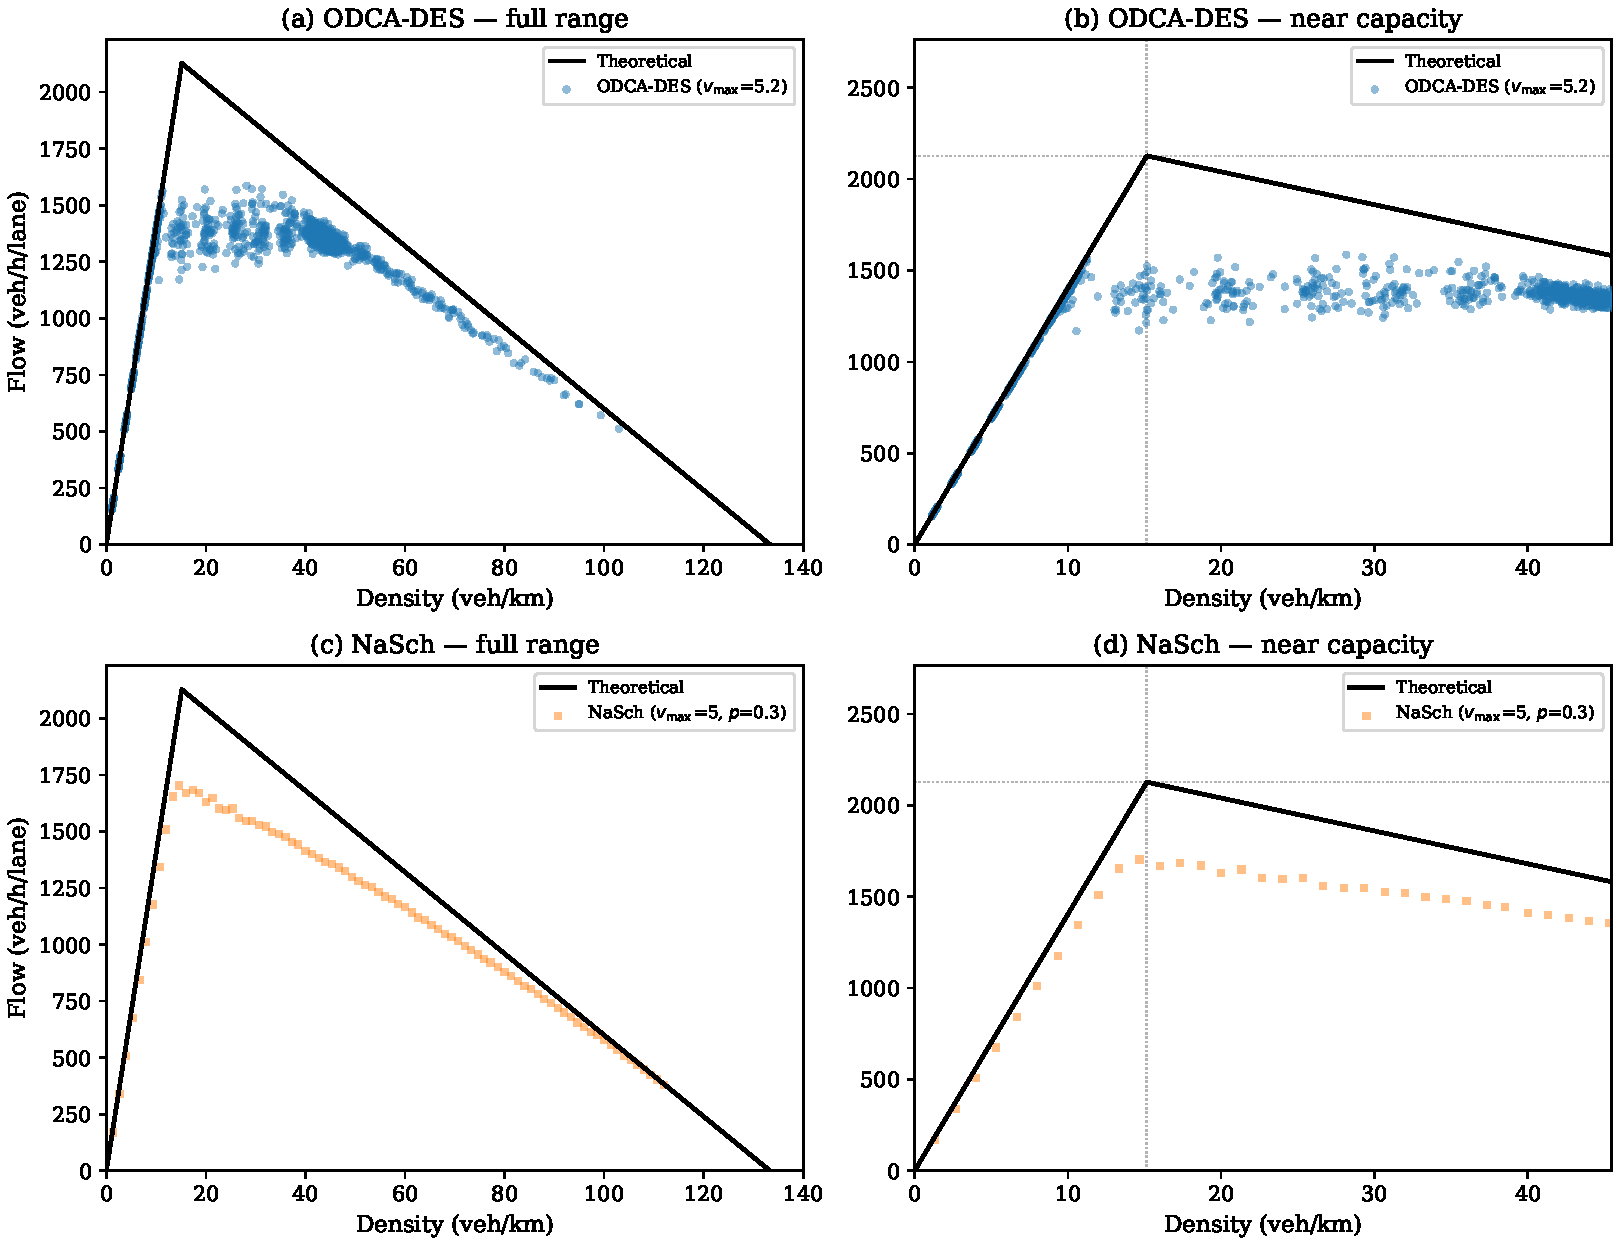
\includegraphics[width=\textwidth]{../figures/fig_fd_theoretical.pdf}
    \caption{Fundamental diagram validation against the theoretical triangular FD ($v_f = 5.2$\,cells/s, $\tau = 1.5$\,s, $q_{\max} = 2127$\,veh/h). Top row: ODCA-DES (continuous speeds, $v_{\max} = 5.2$) produces a smooth envelope \DIFdelbeginFL \DIFdelFL{matching the theoretical curve }\DIFdelendFL across (a)~the full density range and (b)~near capacity\DIFaddbeginFL \DIFaddFL{, on the theoretical line in free flow and peaking at 1}{\DIFaddFL{,}}\DIFaddFL{587\,veh/h on this open segment (1}{\DIFaddFL{,}}\DIFaddFL{948--1}{\DIFaddFL{,}}\DIFaddFL{978\,veh/h on a ring road, see text)}\DIFaddendFL . Bottom row: NaSch (integer speeds, $v_{\max} = 5$, $p = 0.3$) produces clustered flow--density points with a staircase congested branch across (c)~the full range and (d)~near capacity.}
    \label{fig:fd_theoretical}
\end{figure}


\subsection{Trajectory Analysis}
\label{sec:exp_trajectories}

The $T(x, n)$ passage-time output enables direct construction of time-space diagrams. For each vehicle, the trajectory is the set of points $\{(\Tarr(c, i),\; c \cdot \ell)\}$, plotted with time on the horizontal axis and position on the vertical axis.

\subsubsection{Free-Flow Trajectories}

Under low demand (\DIFdelbegin \DIFdel{S1 parameters with reduced mainline demand of }\DIFdelend \DIFaddbegin \DIFadd{the baseline parameters of Table~\ref{tab:vehicle_params} with mainline demand reduced to }\DIFaddend 3{,}000\,veh/h), vehicles traverse the segment without significant resource contention. Figure~\ref{fig:tsd}a shows the resulting time-space diagram: trajectories are near-parallel lines with slope $\ell / v_f$, confirming that the event-driven movement process produces uniform free-flow speeds with only minor perturbations from HDV random slowdowns.

\subsubsection{Congestion Formation and Wave Propagation}

Under high demand (S1, 6000\,veh/h mainline + ramp flows), congestion forms upstream of off-ramps where lane-changing vehicles create friction. As shown in Figure~\ref{fig:tsd}b, the time-space diagram reveals \DIFdelbegin \DIFdel{backward-propagating waves as regions where trajectory slopes decrease (lower speed) or become horizontal (stopped vehicles). The measured wave speed is consistent with the theoretical value $w = \ell/\tau$, demonstrating that congestion dynamics emerge naturally from the resource contention mechanism}\DIFdelend \DIFaddbegin \DIFadd{disturbances that move upstream: each vehicle slows where the one ahead slowed, a short distance later in space and time, so the pattern of slope changes drifts backwards against the traffic. Nothing in the model schedules this; it follows from a cell being released $\tau$ after its holder has moved on}\DIFaddend .

\begin{figure}[ht]
    \centering
    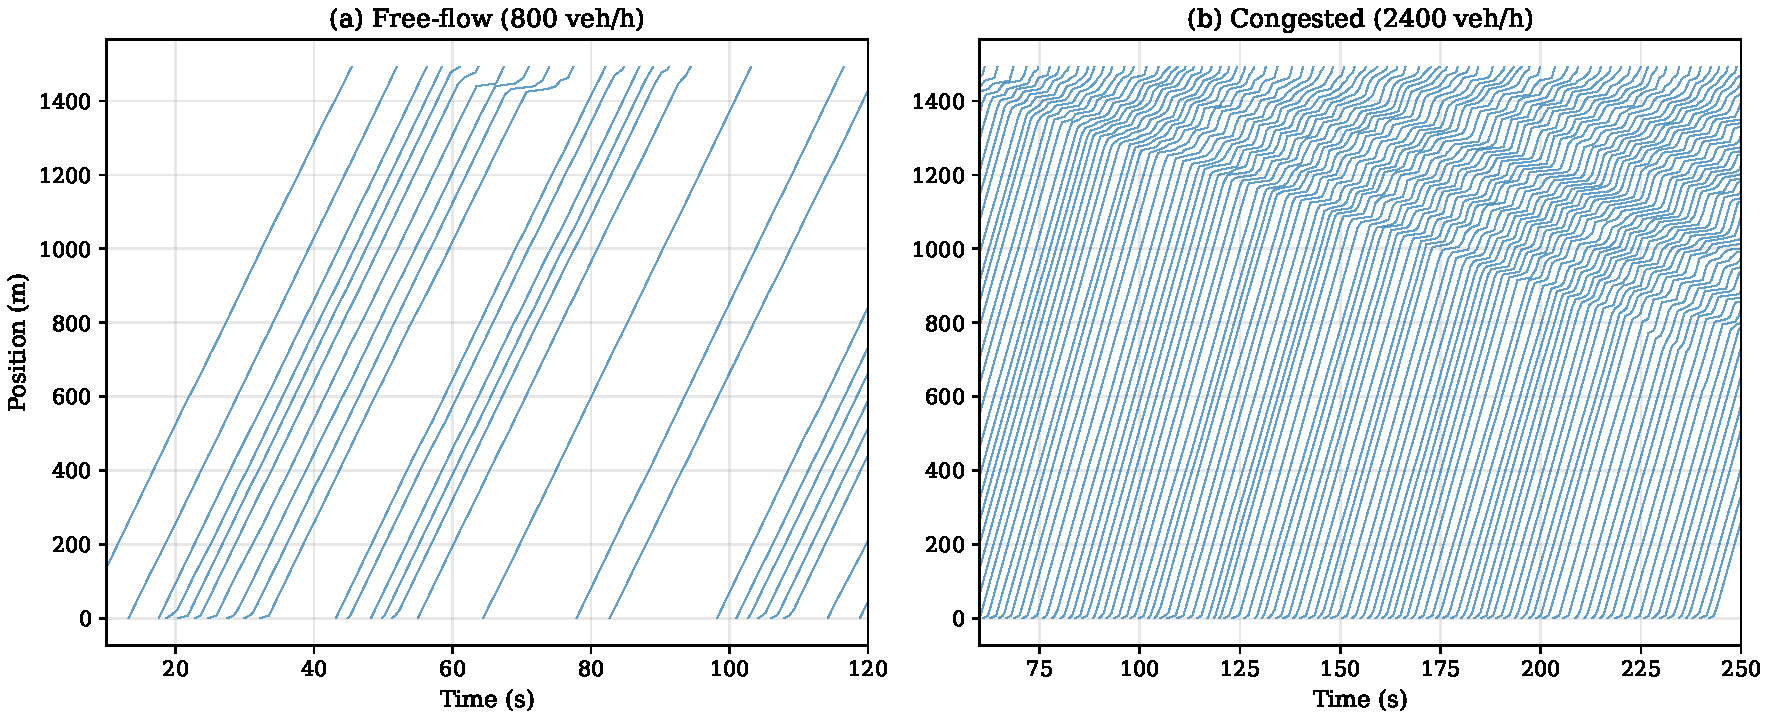
\includegraphics[width=\textwidth]{../figures/fig_tsd_combined.pdf}
    \caption{Time-space diagrams on a single-lane segment. (a)~Free-flow (800\,veh/h): trajectories are near-parallel with slope $v_f = 5.2$\,cells/s ($\approx$140\,km/h), with minor perturbations from HDV random slowdowns. (b)~Congested (2400\,veh/h): trajectory slopes decrease as density exceeds capacity, with backward-propagating waves visible as slope transitions. Trajectories \DIFdelbeginFL \DIFdelFL{colored }\DIFdelendFL \DIFaddbeginFL \DIFaddFL{are coloured }\DIFaddendFL by \DIFaddbeginFL \DIFaddFL{each vehicle's }\DIFaddendFL average speed (blue \DIFdelbeginFL \DIFdelFL{= free flow}\DIFdelendFL \DIFaddbeginFL \DIFaddFL{above 100\,km/h}\DIFaddendFL , orange \DIFdelbeginFL \DIFdelFL{= moderate}\DIFdelendFL \DIFaddbeginFL \DIFaddFL{40--100}\DIFaddendFL , red \DIFdelbeginFL \DIFdelFL{= slow}\DIFdelendFL \DIFaddbeginFL \DIFaddFL{below 40}\DIFaddendFL )\DIFaddbeginFL \DIFaddFL{; at this demand every vehicle averages above 100\,km/h, and the congestion shows as the bending of individual trajectories rather than as slow vehicles}\DIFaddendFL . The \DIFdelbeginFL \DIFdelFL{measured wave speed is consistent with }\DIFdelendFL \DIFaddbeginFL \DIFaddFL{disturbances visible in panel~(b) travel upstream, the direction the theory gives for }\DIFaddendFL $w = \ell/\tau = 0.667$\,cells/s ($\approx$18\,km/h).}
    \label{fig:tsd}
\end{figure}

\subsubsection{Travel Speed vs.\ Running Speed}

The passage-time data naturally distinguishes between travel speed (including waiting) and running speed (movement only). For vehicle $i$ at cell $c$:
\begin{align}
    v_{\text{travel}}(c, i) &= \frac{\ell}{\Tarr(c+1, i) - \Tarr(c, i)} \label{eq:travel_speed} \\
    v_{\text{run}}(c, i) &= \frac{\ell}{\Tarr(c+1, i) - \Tacq(c+1, i)} \label{eq:running_speed}
\end{align}

The difference $v_{\text{run}} - v_{\text{travel}}$ quantifies the delay experienced at each cell. Aggregating this difference across cells and vehicles provides a spatial delay profile, identifying bottleneck locations without requiring predefined detector stations. Figure~\ref{fig:speed_profile} plots both metrics as a function of position along the freeway\DIFdelbegin \DIFdel{; the }\DIFdelend \DIFaddbegin \DIFadd{. Both fall in the first four kilometres, where the on-ramps feed in and the off-ramp traffic works its way to lane~1, and recover to near free flow after off-ramp~2 at 4.125\,km, by which point much of the demand has left the segment. The }\DIFaddend gap between the two curves \DIFdelbegin \DIFdel{reveals that delay concentrates upstream of off-ramps, where mandatory lane changes generate resource contention in the rightmost lanes}\DIFdelend \DIFaddbegin \DIFadd{is a few km/h: at this demand most of the lost time is spent travelling slowly behind a leader rather than waiting for a cell to be released}\DIFaddend .

\begin{figure}[ht]
    \centering
    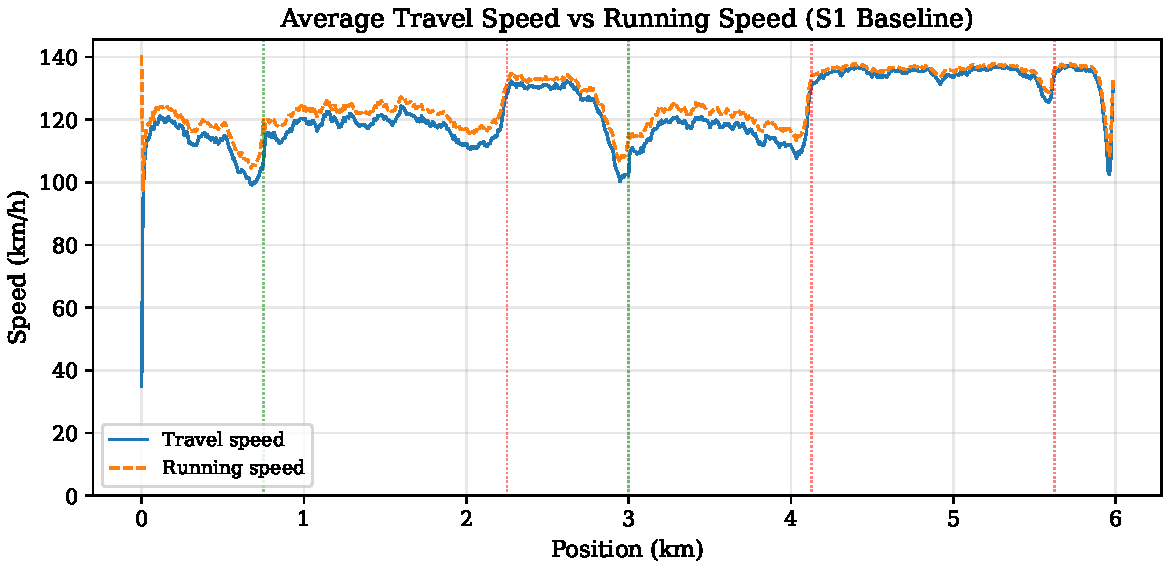
\includegraphics[width=\textwidth]{../figures/fig_speed_profile.pdf}
    \caption{Average travel speed (solid) and running speed (dashed) as a function of position along the freeway (S1\DIFaddbeginFL \DIFaddFL{, one run}\DIFaddendFL ). The gap between the two curves \DIFdelbeginFL \DIFdelFL{represents }\DIFdelendFL \DIFaddbeginFL \DIFaddFL{is the }\DIFaddendFL average cell-level \DIFdelbeginFL \DIFdelFL{delay}\DIFdelendFL \DIFaddbeginFL \DIFaddFL{waiting time}\DIFaddendFL . \DIFdelbeginFL \DIFdelFL{Delay is concentrated upstream of off-ramps }\DIFdelendFL \DIFaddbeginFL \DIFaddFL{Speeds are lowest over the first four kilometres, }\DIFaddendFL where \DIFdelbeginFL \DIFdelFL{lane-changing vehicles create resource contention in }\DIFdelendFL \DIFaddbeginFL \DIFaddFL{ramp traffic and mandatory lane changes concentrate, and recover downstream of off-ramp~2. Dotted lines mark }\DIFaddendFL the \DIFdelbeginFL \DIFdelFL{rightmost lanes}\DIFdelendFL \DIFaddbeginFL \DIFaddFL{on-ramps, dashed lines the off-ramps}\DIFaddendFL .}
    \label{fig:speed_profile}
\end{figure}


\subsection{Mixed Traffic Scenarios}
\label{sec:exp_mixed}

Scenarios S1--S4 are compared across six performance metrics, measured over the full simulation period after a 300-second warm-up interval. All values are means over 20 independent replications (seeds 1--20); 95\% confidence intervals are reported.

\subsubsection{Performance Metrics}

\begin{enumerate}
    \item \textbf{Throughput} ($Q$): \DIFdelbegin \DIFdel{total vehicles exiting }\DIFdelend \DIFaddbegin \DIFadd{vehicles leaving }\DIFaddend the network (via off-ramps and segment end) during the measurement period\DIFaddbegin \DIFadd{, counted by their exit time and scaled to veh/h}\DIFaddend .
    \item \textbf{Average travel time} ($\overline{TT}$): mean time from entry to exit\DIFdelbegin \DIFdel{for all vehiclescompleting their trip}\DIFdelend \DIFaddbegin \DIFadd{, over the same vehicles}\DIFaddend .
    \item \textbf{Average delay} ($\overline{D}$): mean \DIFdelbegin \DIFdel{difference between actual and }\DIFdelend \DIFaddbegin \DIFadd{excess over free-flow travel, summed cell by cell as
    }\begin{equation}
        \DIFadd{D_i = \sum_{c} \max\!\left(0,\; \Tarr(c+1,i) - \Tarr(c,i) - \frac{\ell}{v_f^{(i)}(c)}\right),
        \label{eq:delay}
    }\end{equation}
    \DIFadd{where $v_f^{(i)}(c)$ is the free-flow speed of Eq.~\ref{eq:free_flow_speed}, the vehicle's own maximum speed capped by the limit posted on the cell it is crossing. Delay is therefore what other vehicles cost this one: a cell crossed at its posted limit adds nothing, and a lowered limit changes the }\DIFaddend free-flow travel time \DIFdelbegin \DIFdel{, computed per vehicle as $D_i = \sum_{c} \max(0,\; \Tarr(c+1,i) - \Tarr(c,i) - \ell/v_f)$}\DIFdelend \DIFaddbegin \DIFadd{rather than the delay. Counting per cell rather than as total time minus distance over $v_f$ keeps the extra distance driven by a vehicle that missed its off-ramp out of its delay}\DIFaddend .
    \item \textbf{Lane-change frequency} ($\overline{LC}$): \DIFdelbegin \DIFdel{average number of }\DIFdelend lane changes per vehicle per km\DIFaddbegin \DIFadd{, over the distance the vehicle actually drove}\DIFaddend .
    \item \textbf{Vehicles delayed $> 20$\,s} (\%): fraction of vehicles experiencing total delay exceeding 20\,s.
\DIFdelbegin %DIFDELCMD < \item \textbf{Maximum queue length}%%%
\item%DIFAUXCMD
\DIFdel{: longest contiguous sequence of cells with occupancy (measured in lane~1 upstream of off-ramp~2).
}\DIFdelend \end{enumerate}

\DIFaddbegin \DIFadd{All five are measured over the same set of vehicles: those whose exit time falls in the measurement window. A vehicle already on the road when the warm-up ends therefore counts, which matters at high demand where a large share of the vehicles in the network at any moment entered before the window.
}

\DIFaddend \subsubsection{Results}

Table~\ref{tab:results_mixed} reports the performance metrics across the four scenarios.

\begin{table}[ht]
\centering
\caption{Performance metrics across AV penetration scenarios ($T_{\text{sim}} = 3600$\,s, $N = 20$ replications). Values are means $\pm$ 95\% confidence intervals. The network operates near capacity with per-lane OD flows and three off-ramps requiring mandatory lane changes, creating congested baseline conditions.}
\label{tab:results_mixed}
\begin{tabular}{@{}lcccc@{}}
\toprule
Metric & S1 (0\%) & S2 (30\%) & S3 (50\%) & S4 (70\%) \\
\midrule
Throughput (veh/h) & \DIFdelbeginFL \DIFdelFL{$4{,}494 \pm 14$ }\DIFdelendFL \DIFaddbeginFL \DIFaddFL{$5{,}874 \pm 19$ }\DIFaddendFL & \DIFdelbeginFL \DIFdelFL{$5{,}416 \pm 24$ }\DIFdelendFL \DIFaddbeginFL \DIFaddFL{$6{,}679 \pm 25$ }\DIFaddendFL & \DIFdelbeginFL \DIFdelFL{$6{,}423 \pm 25$ }\DIFdelendFL \DIFaddbeginFL \DIFaddFL{$6{,}972 \pm 34$ }\DIFaddendFL & \DIFdelbeginFL \DIFdelFL{$6{,}664 \pm 48$ }\DIFdelendFL \DIFaddbeginFL \DIFaddFL{$6{,}983 \pm 34$ }\DIFaddendFL \\
Avg.\ travel time (s) & \DIFdelbeginFL \DIFdelFL{$380.8 \pm 6.5$ }\DIFdelendFL \DIFaddbeginFL \DIFaddFL{$347.4 \pm 5.7$ }\DIFaddendFL & \DIFdelbeginFL \DIFdelFL{$329.7 \pm 6.5$ }\DIFdelendFL \DIFaddbeginFL \DIFaddFL{$250.4 \pm 12.2$ }\DIFaddendFL & \DIFdelbeginFL \DIFdelFL{$235.2 \pm 10.2$ }\DIFdelendFL \DIFaddbeginFL \DIFaddFL{$159.3 \pm 1.0$ }\DIFaddendFL & \DIFdelbeginFL \DIFdelFL{$158.1 \pm 1.1$ }\DIFdelendFL \DIFaddbeginFL \DIFaddFL{$141.6 \pm 0.4$ }\DIFaddendFL \\
Avg.\ delay (s) & \DIFdelbeginFL \DIFdelFL{$254.1 \pm 6.6$ }\DIFdelendFL \DIFaddbeginFL \DIFaddFL{$216.6 \pm 5.8$ }\DIFaddendFL & \DIFdelbeginFL \DIFdelFL{$201.3 \pm 6.6$ }\DIFdelendFL \DIFaddbeginFL \DIFaddFL{$119.1 \pm 12.2$ }\DIFaddendFL & \DIFdelbeginFL \DIFdelFL{$105.0 \pm 10.3$ }\DIFdelendFL \DIFaddbeginFL \DIFaddFL{$27.9 \pm 0.9$ }\DIFaddendFL & \DIFdelbeginFL \DIFdelFL{$27.6 \pm 1.1$ }\DIFdelendFL \DIFaddbeginFL \DIFaddFL{$10.2 \pm 0.3$ }\DIFaddendFL \\
LC frequency (/veh/km) & \DIFdelbeginFL \DIFdelFL{$4.89 \pm 0.02$ }\DIFdelendFL \DIFaddbeginFL \DIFaddFL{$2.53 \pm 0.01$ }\DIFaddendFL & \DIFdelbeginFL \DIFdelFL{$3.49 \pm 0.02$ }\DIFdelendFL \DIFaddbeginFL \DIFaddFL{$1.99 \pm 0.04$ }\DIFaddendFL & \DIFdelbeginFL \DIFdelFL{$2.23 \pm 0.04$ }\DIFdelendFL \DIFaddbeginFL \DIFaddFL{$1.20 \pm 0.01$ }\DIFaddendFL & \DIFdelbeginFL \DIFdelFL{$1.22 \pm 0.01$ }\DIFdelendFL \DIFaddbeginFL \DIFaddFL{$0.72 \pm 0.01$ }\\
\DIFaddFL{Vehicles delayed $>20$\,s (\%) }& \DIFaddFL{$99.9 \pm 0.0$ }& \DIFaddFL{$97.6 \pm 0.6$ }& \DIFaddFL{$66.3 \pm 2.2$ }& \DIFaddFL{$9.9 \pm 1.0$ }\DIFaddendFL \\
\bottomrule
\end{tabular}
\end{table}

Based on the analytical capacity expression (Eq.~\ref{eq:mixed_capacity}), the expected theoretical lane capacities are:

\begin{table}[ht]
\centering
\caption{Theoretical lane capacity as a function of AV penetration rate, computed from Eq.~\eqref{eq:mixed_capacity} with $v_f = 5.2$\,cells/s, $\tau_{\text{HDV}} = 1.5$\,s, $\tau_{\text{AV}} = 0.5$\,s, $\ell = 1$\,cell.}
\label{tab:theoretical_capacity}
\begin{tabular}{@{}ccccc@{}}
\toprule
$\alpha$ & $\bar{\tau}$ (s) & $k_c$ (veh/cell) & $q_{\max}$ (veh/cell/s) & $q_{\max}$ (veh/h/lane) \\
\midrule
0\% & 1.50 & 0.114 & 0.591 & 2127 \\
30\% & 1.20 & 0.138 & 0.718 & 2586 \\
50\% & 1.00 & 0.161 & 0.839 & 3019 \\
70\% & 0.80 & 0.194 & 1.008 & 3628 \\
\bottomrule
\end{tabular}
\end{table}

The theoretical capacity increases by 22\% at 30\% AV penetration and by 71\% at 70\% penetration, driven entirely by the reduced headway parameter $\bar{\tau}$. Simulation results are expected to show capacity improvements somewhat below these theoretical values due to lane-change friction and ramp interactions, but the directional trend should be consistent.

\subsubsection{Discussion}

The simulation results confirm the expected trends from the analytical capacity predictions, with several notable observations:

\paragraph{Throughput.} Network throughput increases \DIFdelbegin \DIFdel{monotonically }\DIFdelend with AV penetration, from \DIFdelbegin \DIFdel{$4{,}494 \pm 14$}\DIFdelend \DIFaddbegin \DIFadd{$5{,}874 \pm 19$}\DIFaddend \,veh/h at $\alpha = 0\%$ to \DIFdelbegin \DIFdel{$6{,}664 \pm 48$}\DIFdelend \DIFaddbegin \DIFadd{$6{,}983 \pm 34$}\DIFaddend \,veh/h at $\alpha = 70\%$, \DIFdelbegin \DIFdel{a 48\% improvement. The }\DIFdelend \DIFaddbegin \DIFadd{an 18.9\% improvement, and the }\DIFaddend confidence intervals are tight (coefficient of variation \DIFdelbegin \DIFdel{$< 1.6\%$ in all scenarios), confirming that }\DIFdelend \DIFaddbegin \DIFadd{0.7--1.1\%), so }\DIFaddend 20 replications \DIFdelbegin \DIFdel{provide sufficient statistical resolution. The improvement }\DIFdelend \DIFaddbegin \DIFadd{resolve the differences comfortably. Most of the gain is already realised at 30\% AV ($6{,}679 \pm 25$, that is 13.7\%), and the last two scenarios are within 0.5\% of each other. The reason is that the network runs out of demand before it runs out of capacity: mainline and ramps offer 7}{\DIFadd{,}}\DIFadd{000\,veh/h, so $6{,}983$\,veh/h at $\alpha = 70\%$ }\DIFaddend is \DIFdelbegin \DIFdel{below }\DIFdelend \DIFaddbegin \DIFadd{99.8\% of everything that asks to enter. The all-HDV baseline, by contrast, serves 83.9\% of the offered demand and holds the rest back in the origin queues. The measured improvement is therefore a lower bound on the capacity effect: }\DIFaddend the theoretical 71\% capacity increase (Table~\ref{tab:theoretical_capacity}) \DIFdelbegin \DIFdel{, which assumes homogeneous mixed traffic without lane-change friction. The gap is attributable to ramp interactions and mandatory lane changes---vehicles destined for off-ramps must merge to the rightmost lane, creating cross-lane friction irrespective of vehicle type}\DIFdelend \DIFaddbegin \DIFadd{cannot show up in a throughput figure that the demand caps. Where the extra capacity does show up is in delay, which keeps falling after throughput has saturated}\DIFaddend . Figure~\ref{fig:throughput_bar} visualizes the throughput and delay trends with 95\% confidence intervals.

\paragraph{Delay.} Average delay drops from \DIFdelbegin \DIFdel{$254.1 \pm 6.6$}\DIFdelend \DIFaddbegin \DIFadd{$216.6 \pm 5.8$}\DIFaddend \,s to \DIFdelbegin \DIFdel{$27.6 \pm 1.1$}\DIFdelend \DIFaddbegin \DIFadd{$10.2 \pm 0.3$}\DIFaddend \,s as AV penetration increases from 0\% to 70\%, \DIFdelbegin \DIFdel{an 89\% reduction}\DIFdelend \DIFaddbegin \DIFadd{a 95\% reduction, and the share of vehicles delayed by more than 20\,s falls from essentially all of them (99.9\%) to 9.9\%}\DIFaddend . The high baseline delay reflects the congested operating conditions: the per-lane OD flows with destination distributions require substantial lane-changing activity, and the combined mainline and ramp demand (7{,}000\,veh/h) loads the network near its effective capacity. The event-driven driver process enables vehicles to respond immediately to changing gaps rather than waiting for fixed evaluation intervals, and at 70\% AV penetration the shorter headway ($\tau = 0.5$\,s vs.\ 1.5\,s) significantly reduces car-following delays throughout the network. Figure~\ref{fig:travel_time} presents the average travel time across scenarios.

\paragraph{Lane-change frequency.} Lane-change frequency \emph{decreases} with AV penetration (Table~\ref{tab:results_mixed}). Because AVs perform only mandatory lane changes, increasing AV penetration eliminates discretionary lane-change friction. The remaining lane changes are driven entirely by route requirements (off-ramp exits), and AVs' shorter headways ($\tau = 0.5$\,s) create more available gaps for these mandatory maneuvers, reducing queuing behind slower vehicles in the target lane.

\begin{figure}[ht]
    \centering
    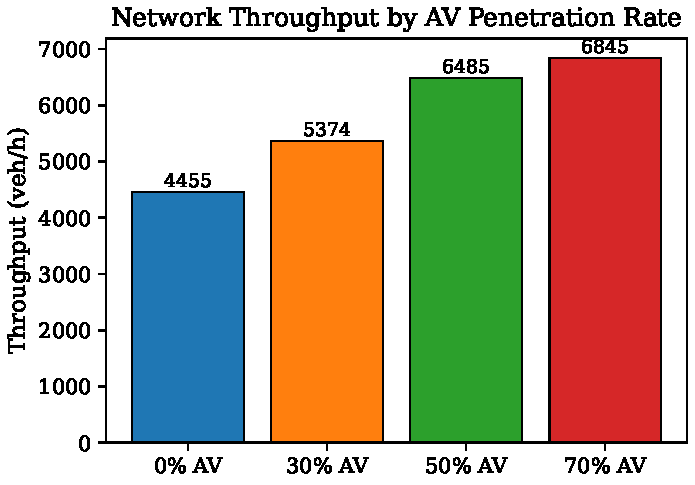
\includegraphics[width=\textwidth]{../figures/fig_throughput_bar.pdf}
    \caption{Network throughput and delay across AV penetration scenarios (S1--S4, $N = 20$ replications). Error bars denote 95\% confidence intervals. Throughput increases \DIFdelbeginFL \DIFdelFL{monotonically }\DIFdelendFL from \DIFdelbeginFL \DIFdelFL{$4{,}494$ }\DIFdelendFL \DIFaddbeginFL \DIFaddFL{$5{,}874$ }\DIFaddendFL to \DIFdelbeginFL \DIFdelFL{$6{,}664$}\DIFdelendFL \DIFaddbeginFL \DIFaddFL{$6{,}983$\,veh/h, saturating at the 7}{\DIFaddFL{,}}\DIFaddFL{000}\DIFaddendFL \,veh/h \DIFaddbeginFL \DIFaddFL{offered demand}\DIFaddendFL , while delay decreases from \DIFdelbeginFL \DIFdelFL{254 }\DIFdelendFL \DIFaddbeginFL \DIFaddFL{217 }\DIFaddendFL to \DIFdelbeginFL \DIFdelFL{28}\DIFdelendFL \DIFaddbeginFL \DIFaddFL{10}\DIFaddendFL \,s.}
    \label{fig:throughput_bar}
\end{figure}

\begin{figure}[ht]
    \centering
    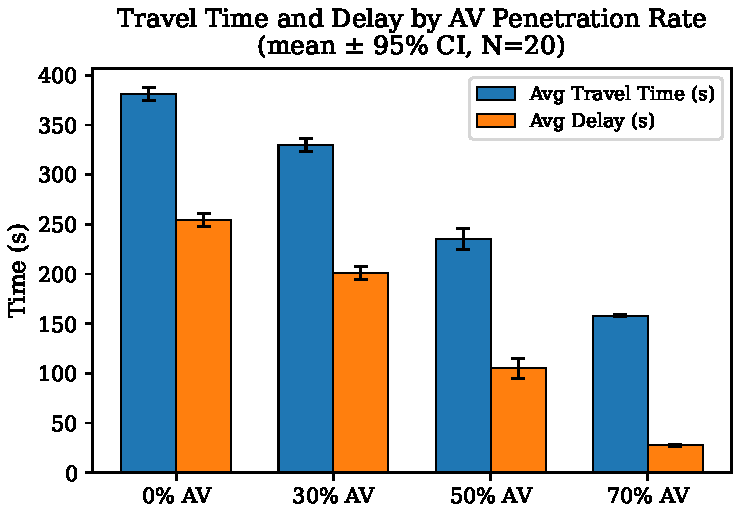
\includegraphics[width=\textwidth]{../figures/fig_travel_time.pdf}
    \caption{Average travel time across AV penetration scenarios (S1--S4, $N = 20$ replications). Error bars denote 95\% confidence intervals. Travel time decreases from \DIFdelbeginFL \DIFdelFL{381}\DIFdelendFL \DIFaddbeginFL \DIFaddFL{347}\DIFaddendFL \,s (S1) to \DIFdelbeginFL \DIFdelFL{158}\DIFdelendFL \DIFaddbeginFL \DIFaddFL{142}\DIFaddendFL \,s (S4)\DIFaddbeginFL \DIFaddFL{. Trips end at three off-ramps and at the segment end}\DIFaddendFL , \DIFdelbeginFL \DIFdelFL{approaching }\DIFdelendFL \DIFaddbeginFL \DIFaddFL{so the reference is not }\DIFaddendFL the full-segment free-flow \DIFdelbeginFL \DIFdelFL{travel }\DIFdelendFL time of 154\,s \DIFaddbeginFL \DIFaddFL{but the demand-weighted free-flow trip time of 131\,s, which S4 exceeds by 8\%. The latter is the mean of each origin--destination pair's free-flow time $\ell\,\Delta c / v_f$ weighted by its flow }\DIFaddendFL (\DIFdelbeginFL \DIFdelFL{$= 800 \cdot 7.5\,\text{m}\;/\;(5.2 \times 7.5\,\text{m/s})$}\DIFdelendFL \DIFaddbeginFL \DIFaddFL{Section~\ref{sec:demand}}\DIFaddendFL )\DIFaddbeginFL \DIFaddFL{; it is shorter than 154\,s because most traffic leaves at off-ramps 1 to 3 rather than driving the full 800 cells, and it is reproduced by }\texttt{\DIFaddFL{code/manuscript\_numbers.py}}\DIFaddendFL .}
    \label{fig:travel_time}
\end{figure}

\paragraph{Computational note.} Wall-clock times range from \DIFdelbegin \DIFdel{277}\DIFdelend \DIFaddbegin \DIFadd{142}\DIFaddend \,s (S4) to \DIFdelbegin \DIFdel{802}\DIFdelend \DIFaddbegin \DIFadd{166}\DIFaddend \,s (\DIFdelbegin \DIFdel{S1}\DIFdelend \DIFaddbegin \DIFadd{S2}\DIFaddend ) for 3{,}600\,s of simulated time\DIFdelbegin \DIFdel{. The }\DIFdelend \DIFaddbegin \DIFadd{, that is 22--25 times faster than real time on one core. The four scenarios are within 17\% of each other: congestion in the }\DIFaddend all-HDV \DIFdelbegin \DIFdel{baseline is slowest because heavy congestion generates the most resource-contention events. As AV penetration increases, reduced lane-change friction and shorter headways alleviate congestion, decreasing the total event count despite the AV controller's }\DIFdelend \DIFaddbegin \DIFadd{baseline adds contention events, and AV penetration adds controller decisions at }\DIFaddend 10\,Hz\DIFdelbegin \DIFdel{evaluation frequency}\DIFdelend \DIFaddbegin \DIFadd{, so the two effects largely cancel. Section~\ref{sec:exp_event_count} takes the event counts apart}\DIFaddend .



\subsection{Bottleneck Analysis: Lane-Drop Scenario}
\label{sec:exp_bottleneck}

To evaluate the framework's performance under capacity-reducing geometry, we simulate a 3-lane, \DIFdelbegin \DIFdel{6}\DIFdelend \DIFaddbegin \DIFadd{4.5}\DIFaddend \,km freeway segment \DIFdelbegin \DIFdel{where the rightmost lane drops at the midpoint }\DIFdelend \DIFaddbegin \DIFadd{(600 cells) where the leftmost lane is closed from the midpoint (cell~300) to the end}\DIFaddend , forcing all \DIFdelbegin \DIFdel{lane-1 }\DIFdelend \DIFaddbegin \DIFadd{lane-3 }\DIFaddend traffic to merge into lanes~\DIFdelbegin \DIFdel{2--3}\DIFdelend \DIFaddbegin \DIFadd{1--2. The closure is a set of blocked cells, the same mechanism used for the incident of Section~\ref{sec:exp_incident}, and the segment starts with vehicles placed every 25 cells per lane so the merge is loaded from the first second}\DIFaddend . Demand is 3{,}600\,veh/h (1{,}200\,veh/h/lane), and AV penetration is varied across 0\%, 30\%, 50\%, and 70\%. Each scenario is run with 20 independent replications.

Table~\ref{tab:results_bottleneck} summarizes the results.

\begin{table}[ht]
\centering
\caption{Bottleneck performance metrics ($N = 20$ replications). Values are means $\pm$ 95\% confidence intervals. BN$_\alpha$ denotes the bottleneck scenario at AV penetration $\alpha$.}
\label{tab:results_bottleneck}
\begin{tabular}{@{}lcccc@{}}
\toprule
Metric & BN$_{0\%}$ & BN$_{30\%}$ & BN$_{50\%}$ & BN$_{70\%}$ \\
\midrule
Throughput (veh/h) & \DIFdelbeginFL \DIFdelFL{$1{,}341 \pm 111$ }\DIFdelendFL \DIFaddbeginFL \DIFaddFL{$2{,}501 \pm 11$ }\DIFaddendFL & \DIFdelbeginFL \DIFdelFL{$1{,}569 \pm 99$ }\DIFdelendFL \DIFaddbeginFL \DIFaddFL{$3{,}127 \pm 23$ }\DIFaddendFL & \DIFdelbeginFL \DIFdelFL{$1{,}773 \pm 164$ }\DIFdelendFL \DIFaddbeginFL \DIFaddFL{$3{,}571 \pm 34$ }\DIFaddendFL & \DIFdelbeginFL \DIFdelFL{$1{,}780 \pm 174$ }\DIFdelendFL \DIFaddbeginFL \DIFaddFL{$3{,}602 \pm 41$ }\\
\DIFaddFL{Avg.\ travel time (s) }& \DIFaddFL{$378.2 \pm 7.8$ }& \DIFaddFL{$236.5 \pm 11.6$ }& \DIFaddFL{$133.3 \pm 2.1$ }& \DIFaddFL{$121.3 \pm 0.3$ }\DIFaddendFL \\
Avg.\ delay (s) & \DIFdelbeginFL \DIFdelFL{$318.1 \pm 32.0$ }\DIFdelendFL \DIFaddbeginFL \DIFaddFL{$263.0 \pm 7.8$ }\DIFaddendFL & \DIFdelbeginFL \DIFdelFL{$320.3 \pm 43.2$ }\DIFdelendFL \DIFaddbeginFL \DIFaddFL{$121.3 \pm 11.6$ }\DIFaddendFL & \DIFdelbeginFL \DIFdelFL{$214.7 \pm 42.9$ }\DIFdelendFL \DIFaddbeginFL \DIFaddFL{$18.1 \pm 2.1$ }\DIFaddendFL & \DIFdelbeginFL \DIFdelFL{$142.3 \pm 42.6$ }\DIFdelendFL \DIFaddbeginFL \DIFaddFL{$6.1 \pm 0.3$ }\DIFaddendFL \\
LC frequency (/veh/km) & \DIFdelbeginFL \DIFdelFL{$2.11 \pm 0.26$ }\DIFdelendFL \DIFaddbeginFL \DIFaddFL{$1.09 \pm 0.01$ }\DIFaddendFL & \DIFdelbeginFL \DIFdelFL{$1.59 \pm 0.14$ }\DIFdelendFL \DIFaddbeginFL \DIFaddFL{$0.96 \pm 0.02$ }\DIFaddendFL & \DIFdelbeginFL \DIFdelFL{$1.22 \pm 0.14$ }\DIFdelendFL \DIFaddbeginFL \DIFaddFL{$0.59 \pm 0.01$ }\DIFaddendFL & \DIFdelbeginFL \DIFdelFL{$0.74 \pm 0.07$ }\DIFdelendFL \DIFaddbeginFL \DIFaddFL{$0.35 \pm 0.01$ }\\
\DIFaddFL{Vehicles delayed $>20$\,s (\%) }& \DIFaddFL{$97.3 \pm 0.4$ }& \DIFaddFL{$94.2 \pm 2.0$ }& \DIFaddFL{$34.7 \pm 6.2$ }& \DIFaddFL{$2.1 \pm 0.6$ }\DIFaddendFL \\
\bottomrule
\end{tabular}
\end{table}

\paragraph{\DIFdelbegin \DIFdel{Throughput plateau near }\DIFdelend \DIFaddbegin \DIFadd{The two-lane throat stops being the constraint between 30\% and }\DIFaddend 50\% AV\DIFdelbegin \DIFdel{penetration}\DIFdelend .}
\DIFdelbegin \DIFdel{Unlike the open-freeway scenarios (S1--S4), where throughput increases monotonically across the full penetration range, the bottleneck exhibits a throughput plateau above 50\% AV penetration: BN$_{50\%}$ achieves $1{,}773 \pm 164$}\DIFdelend \DIFaddbegin \DIFadd{The lane drop holds the all-HDV stream to $2{,}501 \pm 11$}\DIFaddend \,veh/h\DIFdelbegin \DIFdel{while BN$_{70\%}$ yields $1{,}780 \pm 174$\,veh/h---a difference of 8}\DIFdelend \DIFaddbegin \DIFadd{, that is 69\% of the 3}{\DIFadd{,}}\DIFadd{600}\DIFaddend \,veh/h \DIFdelbegin \DIFdel{with fully overlapping 95\%confidence intervals }\DIFdelend \DIFaddbegin \DIFadd{demand: the rest waits upstream. Throughput then rises to $3{,}127 \pm 23$ at 30\% AV, $3{,}571 \pm 34$ at 50\% and $3{,}602 \pm 41$ at 70\%. The last step is 0.9\% and the two confidence intervals overlap }\DIFaddend (Figure~\ref{fig:bottleneck_throughput})\DIFdelbegin \DIFdel{. The two scenarios are statistically indistinguishable.
}%DIFDELCMD < 

%DIFDELCMD < %%%
\DIFdel{Note that per-vehicle delay at BN$_{30\%}$ ($320.3 \pm 43.2$\,s) is virtually identical to BN$_{0\%}$ ($318.1 \pm 32.0$\,s) despite the 17\% throughput increase; the higher throughput means that more vehicles complete long-delay trips that would have been blocked entirely at BN$_{0\%}$, holding the per-vehicle average delay roughly constant even as aggregate performance improves. The confidence intervals also overlap substantially}\DIFdelend \DIFaddbegin \DIFadd{, but the reason is not that the merge saturates: at 50\% the two remaining lanes already carry 99.2\% of the offered demand, and at 70\% they carry all of it. Between 30\% and 50\% AV the throat stops being the binding constraint, and beyond that point the demand is}\DIFaddend .

\DIFdelbegin \DIFdel{The mechanism underlying the throughput plateau is merge-capacity saturation: at 50\% AVpenetration, the smoother headways of AVs ($\tau = 0.5$}\DIFdelend \DIFaddbegin \DIFadd{Delay makes the same transition visible without the ceiling: $263.0 \pm 7.8$}\DIFaddend \,\DIFdelbegin \DIFdel{s vs.\ 1.5}\DIFdelend \DIFaddbegin \DIFadd{s at 0\% AV, $121.3 \pm 11.6$ at 30\%, $18.1 \pm 2.1$ at 50\% and $6.1 \pm 0.3$ at 70\%, and the share of vehicles delayed by more than 20}\DIFaddend \,s \DIFdelbegin \DIFdel{for HDVs) already enable near-maximum utilization of the two remaining lanes at the merge point. Additional AVs beyond this threshold reduce per-vehicle delay (from $214.7 \pm 42.9$\,s to $142.3 \pm 42.6$\,s) by improving upstream flow conditions, but the downstream capacity at the 2-lane bottleneck throat cannot absorb further throughputgains. This finding is qualitatively consistent with }\DIFdelend \DIFaddbegin \DIFadd{falls from 97.3\% to 2.1\%. The 50\% and 70\% scenarios, indistinguishable in throughput, differ by a factor of three in delay: once every vehicle gets through, what an additional AV buys is time, not flow. This is }\DIFaddend the concavity of the theoretical capacity function $q_{\max}(\alpha)$ (Eq.~\ref{eq:mixed_capacity}) \DIFdelbegin \DIFdel{, in which the marginal headway reduction per additional AV diminishes with increasing $\alpha$; however, the plateau itself reflects merge dynamics at the lane drop that are not captured by the idealized single-stream capacity formula}\DIFdelend \DIFaddbegin \DIFadd{meeting a fixed demand, rather than a property of the merge itself}\DIFaddend .

\DIFdelbegin \DIFdel{The wider confidence intervals in the bottleneck scenarios (}\DIFdelend \DIFaddbegin \DIFadd{Run-to-run variability is larger here than on the open freeway, and it is delay, not throughput, that carries it: the }\DIFaddend coefficient of variation \DIFdelbegin \DIFdel{10--21\% , compared to }\DIFdelend \DIFaddbegin \DIFadd{of throughput stays between 0.9\% and 2.4\% (}\DIFaddend 0.7--1\DIFdelbegin \DIFdel{.6}\DIFdelend \DIFaddbegin \DIFadd{.1}\DIFaddend \% for S1--S4)\DIFdelbegin \DIFdel{reflect the sensitivity of merge dynamics to random vehicle sequencing at the lane drop}\DIFdelend \DIFaddbegin \DIFadd{, while for delay it reaches 24\% at BN$_{50\%}$, where a run either clears the queue before the end of the hour or does not}\DIFaddend . The stochastic order in which HDVs and AVs \DIFdelbegin \DIFdel{arrive at the merge point creates higher run-to-run variability than the distributed ramp interactions of the open-freeway network}\DIFdelend \DIFaddbegin \DIFadd{reach the merge decides that}\DIFaddend .

\begin{figure}[ht]
    \centering
    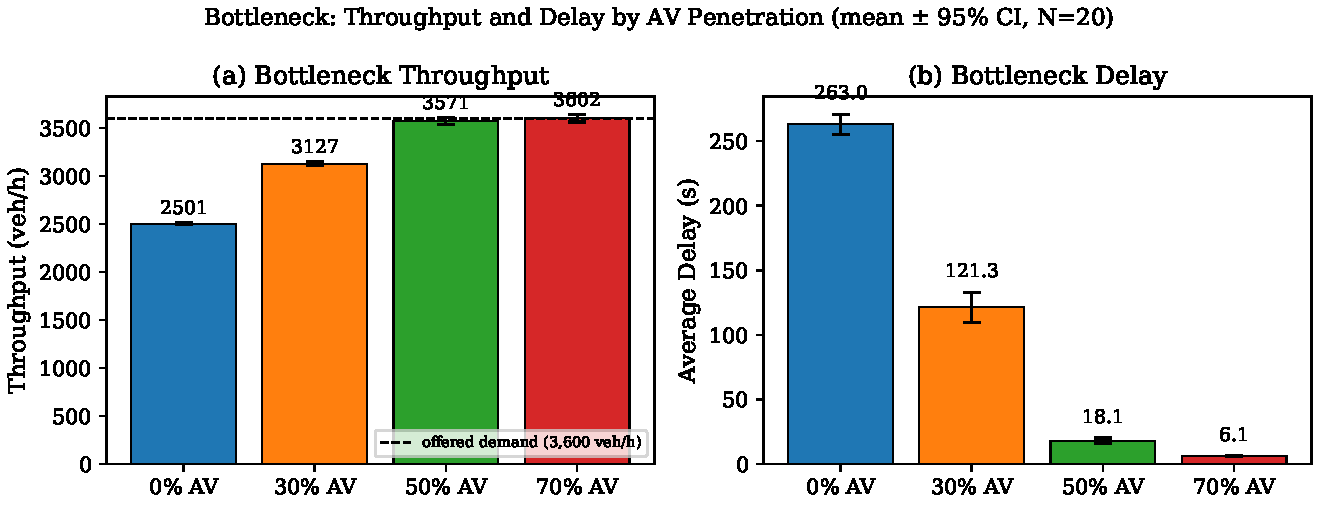
\includegraphics[width=\textwidth]{../figures/fig_bottleneck_throughput.pdf}
    \caption{Bottleneck throughput across AV penetration levels ($N = 20$ replications). Error bars denote 95\% confidence intervals. \DIFdelbeginFL \DIFdelFL{The throughput benefit plateaus near }\DIFdelendFL \DIFaddbeginFL \DIFaddFL{Throughput rises from $2{,}501$ to $3{,}602$\,veh/h and flattens between }\DIFaddendFL 50\% \DIFaddbeginFL \DIFaddFL{and 70\% }\DIFaddendFL AV\DIFdelbeginFL \DIFdelFL{penetration: }\DIFdelendFL \DIFaddbeginFL \DIFaddFL{, where }\DIFaddendFL the \DIFdelbeginFL \DIFdelFL{BN$_{50\%}$ }\DIFdelendFL \DIFaddbeginFL \DIFaddFL{two remaining lanes already carry 99\% of the 3}{\DIFaddFL{,}}\DIFaddFL{600\,veh/h demand (dashed line) }\DIFaddendFL and\DIFdelbeginFL \DIFdelFL{BN$_{70\%}$ confidence intervals overlap almost entirely}\DIFdelendFL , \DIFdelbeginFL \DIFdelFL{indicating no statistically significant throughput gain beyond 50}\DIFdelendFL \DIFaddbeginFL \DIFaddFL{at 70}\DIFaddendFL \%\DIFdelbeginFL \DIFdelFL{in a capacity-constrained merge}\DIFdelendFL \DIFaddbeginFL \DIFaddFL{, all of it; beyond that point the extra capacity shows up as delay reduction, not as flow}\DIFaddendFL .}
    \label{fig:bottleneck_throughput}
\end{figure}


\subsection{Sensitivity to HDV Action Interval}
\label{sec:exp_sensitivity}

The HDV action interval $\delta_{\text{eval}}$ (the maximum time between driver re-evaluations; Section~\ref{sec:driver}) is a key model parameter that controls how frequently human drivers reassess speed and lane-change decisions. The default value of $\delta_{\text{eval}} = 1.0$\,s reflects typical human perception-reaction cycling, but lower values approximate more attentive driving or a finer-grained discrete-time approximation of continuous decision-making.

To quantify the sensitivity of simulation outcomes to this parameter, we run the S1 (all-HDV) scenario at three action-interval values: $\delta_{\text{eval}} \in \{0.25, 0.5, 1.0\}$\,s, with 10 replications at $\delta_{\text{eval}} = 0.25$ and $0.5$\,s and 20 replications at $\delta_{\text{eval}} = 1.0$\,s (the baseline from Section~\ref{sec:exp_mixed}). Table~\ref{tab:sensitivity_ai} reports the results; Figure~\ref{fig:sensitivity_ai} presents the trends graphically.

\begin{table}[ht]
\centering
\caption{Sensitivity of S1 (0\% AV) performance to HDV action interval. Values are means $\pm$ 95\% CI.}
\label{tab:sensitivity_ai}
\begin{tabular}{@{}lccc@{}}
\toprule
Metric & $\delta_{\text{eval}} = 0.25$\,s & $\delta_{\text{eval}} = 0.5$\,s & $\delta_{\text{eval}} = 1.0$\,s \\
\midrule
Throughput (veh/h) & \DIFdelbeginFL \DIFdelFL{$4{,}870 \pm 16$ }\DIFdelendFL \DIFaddbeginFL \DIFaddFL{$6{,}252 \pm 32$ }\DIFaddendFL & \DIFdelbeginFL \DIFdelFL{$4{,}762 \pm 23$ }\DIFdelendFL \DIFaddbeginFL \DIFaddFL{$6{,}164 \pm 26$ }\DIFaddendFL & \DIFdelbeginFL \DIFdelFL{$4{,}494 \pm 14$ }\DIFdelendFL \DIFaddbeginFL \DIFaddFL{$5{,}874 \pm 19$ }\DIFaddendFL \\
Avg.\ travel time (s) & \DIFdelbeginFL \DIFdelFL{$330.2 \pm 4.1$ }\DIFdelendFL \DIFaddbeginFL \DIFaddFL{$326.2 \pm 8.2$ }\DIFaddendFL & \DIFdelbeginFL \DIFdelFL{$346.4 \pm 8.6$ }\DIFdelendFL \DIFaddbeginFL \DIFaddFL{$329.9 \pm 7.7$ }\DIFaddendFL & \DIFdelbeginFL \DIFdelFL{$380.8 \pm 6.5$ }\DIFdelendFL \DIFaddbeginFL \DIFaddFL{$347.4 \pm 5.7$ }\DIFaddendFL \\
Avg.\ delay (s) & \DIFdelbeginFL \DIFdelFL{$202.6 \pm 4.2$ }\DIFdelendFL \DIFaddbeginFL \DIFaddFL{$194.3 \pm 8.1$ }\DIFaddendFL & \DIFdelbeginFL \DIFdelFL{$219.0 \pm 8.6$ }\DIFdelendFL \DIFaddbeginFL \DIFaddFL{$198.6 \pm 7.7$ }\DIFaddendFL & \DIFdelbeginFL \DIFdelFL{$254.1 \pm 6.6$ }\DIFdelendFL \DIFaddbeginFL \DIFaddFL{$216.6 \pm 5.8$ }\DIFaddendFL \\
LC frequency (/veh/km) & \DIFdelbeginFL \DIFdelFL{$4.10 \pm 0.02$ }\DIFdelendFL \DIFaddbeginFL \DIFaddFL{$2.15 \pm 0.01$ }\DIFaddendFL & \DIFdelbeginFL \DIFdelFL{$4.39 \pm 0.03$ }\DIFdelendFL \DIFaddbeginFL \DIFaddFL{$2.30 \pm 0.01$ }\DIFaddendFL & \DIFdelbeginFL \DIFdelFL{$4.89 \pm 0.02$ }\DIFdelendFL \DIFaddbeginFL \DIFaddFL{$2.53 \pm 0.01$ }\DIFaddendFL \\
\bottomrule
\end{tabular}
\end{table}

\begin{figure}[ht]
    \centering
    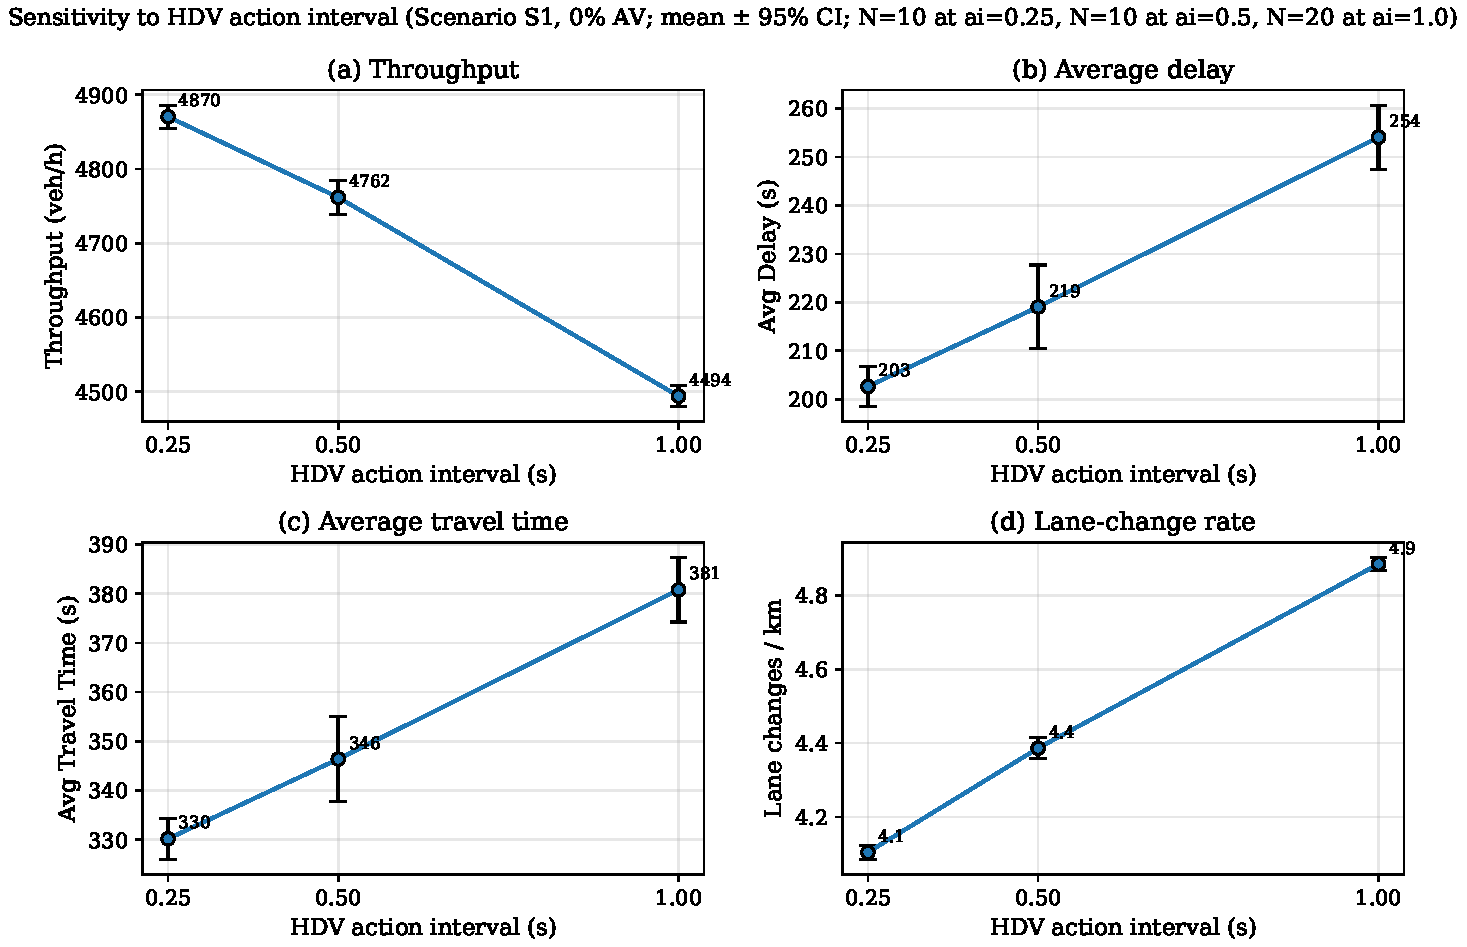
\includegraphics[width=\textwidth]{../figures/fig_sensitivity_action_interval.pdf}
    \caption{Sensitivity of S1 performance metrics to HDV action interval $\delta_{\text{eval}}$. Panels show throughput, average travel time, average delay, and lane-change frequency. Error bars denote 95\% confidence intervals. Reducing the action interval monotonically improves all metrics.}
    \label{fig:sensitivity_ai}
\end{figure}

Reducing the action interval from 1.0\,s to 0.25\,s increases throughput by \DIFdelbegin \DIFdel{8.4}\DIFdelend \DIFaddbegin \DIFadd{6.4}\DIFaddend \% (from \DIFdelbegin \DIFdel{$4{,}494 \pm 14$ to $4{,}870 \pm 16$}\DIFdelend \DIFaddbegin \DIFadd{$5{,}874 \pm 19$ to $6{,}252 \pm 32$}\DIFaddend \,veh/h) and reduces average delay by \DIFdelbegin \DIFdel{20}\DIFdelend \DIFaddbegin \DIFadd{10}\DIFaddend \% (from \DIFdelbegin \DIFdel{$254 \pm 7$ to $203 \pm 4$}\DIFdelend \DIFaddbegin \DIFadd{$217 \pm 6$ to $194 \pm 8$}\DIFaddend \,s). \DIFaddbegin \DIFadd{Most of that comes from the first halving: 0.5\,s already gives $6{,}164 \pm 26$\,veh/h, and the step to 0.25\,s adds 1.4\% more. }\DIFaddend The effect is monotonic across all metrics: finer-grained driver re-evaluation enables smoother speed adjustments and earlier gap exploitation, reducing the stop-and-go oscillations that arise when drivers react to stale state information. Lane-change frequency decreases at lower action intervals, indicating that more responsive drivers maintain better longitudinal flow, reducing the need for discretionary lane changes.

This result has a structural interpretation: as $\delta_{\text{eval}} \to 0$, the event-driven driver process converges toward the continuous-time limit of the Newell car-following model, closing the gap between the discrete-event implementation and the underlying continuous-time theory. The \DIFdelbegin \DIFdel{8.4}\DIFdelend \DIFaddbegin \DIFadd{6.4}\DIFaddend \% throughput improvement from a 4$\times$ reduction in action interval quantifies this structural gap, \DIFdelbegin \DIFdel{suggesting }\DIFdelend \DIFaddbegin \DIFadd{and its concentration in the first halving suggests }\DIFaddend that the default 1.0\,s value is a conservative but reasonable operating point.

\paragraph{Scope note.} This sensitivity analysis is restricted to S1 (all-HDV) because the action interval is an HDV parameter; AVs operate on a fixed 10\,Hz controller cycle irrespective of $\delta_{\text{eval}}$. In mixed-traffic scenarios (S2--S4), HDVs constitute a decreasing fraction of the fleet, so the sensitivity to $\delta_{\text{eval}}$ is proportionally smaller. Additionally, reducing $\delta_{\text{eval}}$ in mixed-traffic scenarios with high event density proved computationally intractable within the experimental budget. Note that the $\delta_{\text{eval}} = 0.25$ and $0.5$\,s scenarios use $N = 10$ replications versus $N = 20$ for the baseline at $\delta_{\text{eval}} = 1.0$\,s; accordingly, the 95\% confidence intervals at the two lower values are computed with fewer degrees of freedom and are somewhat wider than they would be at $N = 20$.


\subsection{Computational Performance}
\label{sec:exp_performance_new}

\subsubsection{Scalability with Network Size}
\label{sec:exp_scalability}

To assess how the event-driven architecture scales with network size, we simulate the S1 (all-HDV) scenario on networks of increasing size: 200, 400, 800, 1{,}600, and 3{,}200 cells per lane (4 lanes each, yielding 800 to 12{,}800 total cells), with 3 seeds per configuration. All networks use the same demand density and simulation duration ($T_{\text{sim}} = 1{,}800$\,s). Table~\ref{tab:scalability} reports the results; Figure~\ref{fig:scalability} presents the scaling trends.

\begin{table}[ht]
\centering
\caption{Computational scalability across network sizes (S1, all-HDV, $N = 3$ seeds per size, $T_{\text{sim}} = 1{,}800$\,s\DIFaddbeginFL \DIFaddFL{, means over seeds}\DIFaddendFL ). Total cells = num\_cells $\times$ 4 lanes. \DIFaddbeginFL \DIFaddFL{Demand is the same at every size (3}{\DIFaddFL{,}}\DIFaddFL{040 vehicles generated), so a longer network means longer trips rather than more vehicles.}\DIFaddendFL }
\label{tab:scalability}
\begin{tabular}{@{}rrrrl@{}}
\toprule
Cells/lane & Total cells & \DIFdelbeginFL \DIFdelFL{Events ($\times 10^3$}\DIFdelendFL \DIFaddbeginFL \DIFaddFL{SimPy events ($\times 10^6$}\DIFaddendFL ) & Wall clock (s) & Realtime ratio \\
\midrule
200 & 800 & \DIFdelbeginFL \DIFdelFL{394 }\DIFdelendFL \DIFaddbeginFL \DIFaddFL{6.01 }\DIFaddendFL & \DIFdelbeginFL \DIFdelFL{227 }\DIFdelendFL \DIFaddbeginFL \DIFaddFL{18.0 }\DIFaddendFL & \DIFdelbeginFL \DIFdelFL{$8.0\times$ }\DIFdelendFL \DIFaddbeginFL \DIFaddFL{$100.3\times$ }\DIFaddendFL \\
400 & 1{,}600 & \DIFdelbeginFL \DIFdelFL{619 }\DIFdelendFL \DIFaddbeginFL \DIFaddFL{11.31 }\DIFaddendFL & \DIFdelbeginFL \DIFdelFL{370 }\DIFdelendFL \DIFaddbeginFL \DIFaddFL{35.9 }\DIFaddendFL & \DIFdelbeginFL \DIFdelFL{$5.2\times$ }\DIFdelendFL \DIFaddbeginFL \DIFaddFL{$50.2\times$ }\DIFaddendFL \\
800 & 3{,}200 & \DIFdelbeginFL \DIFdelFL{910 }\DIFdelendFL \DIFaddbeginFL \DIFaddFL{20.78 }\DIFaddendFL & \DIFdelbeginFL \DIFdelFL{448 }\DIFdelendFL \DIFaddbeginFL \DIFaddFL{71.2 }\DIFaddendFL & \DIFdelbeginFL \DIFdelFL{$4.1\times$ }\DIFdelendFL \DIFaddbeginFL \DIFaddFL{$25.3\times$ }\DIFaddendFL \\
1{,}600 & 6{,}400 & \DIFdelbeginFL \DIFdelFL{1}%DIFDELCMD < {%%%
\DIFdelFL{,}%DIFDELCMD < }%%%
\DIFdelFL{364 }\DIFdelendFL \DIFaddbeginFL \DIFaddFL{37.87 }\DIFaddendFL & \DIFdelbeginFL \DIFdelFL{786 }\DIFdelendFL \DIFaddbeginFL \DIFaddFL{147.1 }\DIFaddendFL & \DIFdelbeginFL \DIFdelFL{$2.3\times$ }\DIFdelendFL \DIFaddbeginFL \DIFaddFL{$12.2\times$ }\DIFaddendFL \\
3{,}200 & 12{,}800 & \DIFdelbeginFL \DIFdelFL{1}%DIFDELCMD < {%%%
\DIFdelFL{,}%DIFDELCMD < }%%%
\DIFdelFL{935 }\DIFdelendFL \DIFaddbeginFL \DIFaddFL{65.05 }\DIFaddendFL & \DIFdelbeginFL \DIFdelFL{1}%DIFDELCMD < {%%%
\DIFdelFL{,}%DIFDELCMD < }%%%
\DIFdelFL{533 }\DIFdelendFL \DIFaddbeginFL \DIFaddFL{304.3 }\DIFaddendFL & \DIFdelbeginFL \DIFdelFL{$1.2\times$ }\DIFdelendFL \DIFaddbeginFL \DIFaddFL{$5.9\times$ }\DIFaddendFL \\
\bottomrule
\end{tabular}
\end{table}

\begin{figure}[ht]
    \centering
    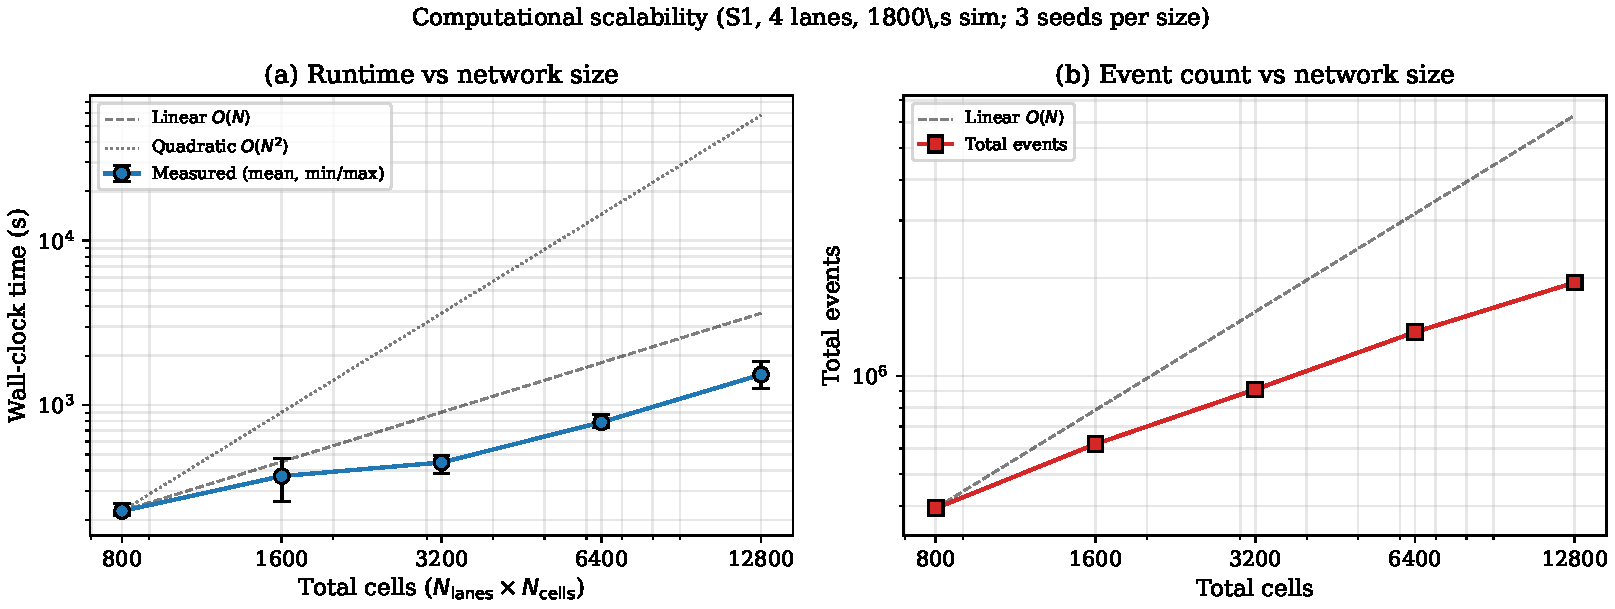
\includegraphics[width=\textwidth]{../figures/fig_scalability.pdf}
    \caption{Computational scalability of ODCA-DES. Left: total events and wall-clock time vs.\ network size (log--log scale). Right: realtime ratio vs.\ total cells. Event count scales sub-linearly with network size \DIFaddbeginFL \DIFaddFL{(empirical exponent 0.86)}\DIFaddendFL , reflecting event locality in the DES architecture.}
    \label{fig:scalability}
\end{figure}

The \DIFdelbegin \DIFdel{total }\DIFdelend event count increases by a factor of \DIFdelbegin \DIFdel{4.9$\times$ for a 16$\times$ increase in cell count }\DIFdelend \DIFaddbegin \DIFadd{10.8 for a 16-fold increase in length }\DIFaddend (200 to 3{,}200 cells per lane), \DIFdelbegin \DIFdel{confirming sub-linear scaling (empirical exponent $\approx 0.57$, i.e. , $O(n^{0.57})$). This is a direct consequence of event locality: events are generated by vehicle interactions, not by grid traversal, so expanding the network with proportional demandincreases the number of interacting vehicle pairs sub-linearly as congestion remains localized}\DIFdelend \DIFaddbegin \DIFadd{an empirical exponent of 0.86. The demand is the same at every size, so this is the cost of longer trips and not of more traffic: each vehicle crosses 16 times as many cells, and each cell crossing costs the same handful of events. The shortfall from 16 is where the event-driven design shows: the short network is congested with the same demand, and contention there adds waits and re-evaluations per cell that the long, free-flowing network does not pay}\DIFaddend . Wall-clock time \DIFdelbegin \DIFdel{increases by 6.8$\times$ over the same range, reflecting both }\DIFdelend \DIFaddbegin \DIFadd{grows by 16.9, faster than }\DIFaddend the event count\DIFdelbegin \DIFdel{growth and the increased overhead of managing a larger event calendar}\DIFdelend \DIFaddbegin \DIFadd{, because a larger network keeps more processes and a longer event calendar alive, so an event costs more to schedule as the network grows}\DIFaddend . The realtime ratio \DIFdelbegin \DIFdel{decreases from $8.0\times$ }\DIFdelend \DIFaddbegin \DIFadd{falls from $100\times$ }\DIFaddend (800 total cells) to \DIFdelbegin \DIFdel{$1.2\times$ on average }\DIFdelend \DIFaddbegin \DIFadd{$5.9\times$ }\DIFaddend (12{,}800 total cells)\DIFdelbegin \DIFdel{, maintaining near-realtime or faster execution across the tested network sizes}\DIFdelend \DIFaddbegin \DIFadd{: every size tested runs faster than real time on one core}\DIFaddend .


\subsubsection{Event Count Analysis}
\label{sec:exp_event_count}

To assess the computational characteristics of the event-driven approach on a per-scenario basis, we compare the number of simulation events and wall-clock execution time against a timestep-equivalent simulation on the same 4-lane, 800-cell network.

In a timestep-based simulator with update interval $\Delta t$, the number of update operations is:
\begin{equation}
    N_{\text{timestep}} = \bar{N}_{\text{vehicles}} \times \frac{T_{\text{sim}}}{\Delta t}
    \label{eq:timestep_count}
\end{equation}
where $\bar{N}_{\text{vehicles}}$ is the average number of vehicles simultaneously present in the network. Every vehicle is evaluated at every timestep regardless of its interaction state.

In ODCA-DES \DIFdelbegin \DIFdel{, the event count depends on the traffic state.
Each vehicle generates:
}%DIFDELCMD < \begin{itemize}
%DIFDELCMD <     \item %%%
\DIFdel{Movement events: two }\DIFdelend \DIFaddbegin \DIFadd{the work splits into two kinds, and they should be counted separately.
}

\emph{\DIFadd{Movement events}} \DIFadd{implement the resource protocol: }\DIFaddend per cell traversed\DIFdelbegin \DIFdel{(seize+ release), giving $2 \times C_{\text{traversed}}$ events per vehicle .
    }%DIFDELCMD < \item %%%
\DIFdel{Driver events: one per perception-delay interval, giving $T_{\text{trip}} / \delta_{\text{percept}}$ events per vehicle.
}%DIFDELCMD < \item %%%
\DIFdel{Wait events: additional events when resource contention occurs (zero in free flow, proportional to congestion severity) .
}%DIFDELCMD < \end{itemize}
%DIFDELCMD < %%%
\DIFdelend \DIFaddbegin \DIFadd{, a request, a seize, the traversal timeout (or several of them, when the vehicle is slow enough to be re-timed while crossing) and the delayed release, plus a wait whenever the next cell is held. They have no counterpart in a timestep model, which moves a vehicle by arithmetic on its position, and they dominate the total: the scenarios below execute 38--41 million SimPy events per hour of simulated traffic, almost all of them movement.
}

\emph{\DIFadd{Decision events}} \DIFadd{are the behavioural layer, and they are what a timestep model repeats for every vehicle at every step: a speed evaluation (car following when a leader is in range, free flow otherwise) and a direction evaluation per driver wake-up, or per controller cycle for an AV.
}\DIFaddend 

Table~\ref{tab:computational} compares the event counts and wall-clock times across the S1--S4 scenarios.

\begin{table}[ht]
\centering
\caption{Computational performance\DIFdelbeginFL \DIFdelFL{comparison. Events counted for the full simulation }\DIFdelendFL \DIFaddbeginFL \DIFaddFL{, one run per scenario on a quiet machine }\DIFaddendFL ($T_{\text{sim}} = 3600$\,s\DIFaddbeginFL \DIFaddFL{, 4 lanes, 800 cells, seed 42}\DIFaddendFL )\DIFdelbeginFL \DIFdelFL{on }\DIFdelendFL \DIFaddbeginFL \DIFaddFL{. SimPy events are every event }\DIFaddendFL the \DIFdelbeginFL \DIFdelFL{4-lane, 800-cell network}\DIFdelendFL \DIFaddbeginFL \DIFaddFL{calendar processed; speed evaluations are the driver decisions}\DIFaddendFL . \DIFdelbeginFL \DIFdelFL{Timestep }\DIFdelendFL \DIFaddbeginFL \DIFaddFL{The timestep row is the }\DIFaddendFL baseline \DIFdelbeginFL \DIFdelFL{uses }\DIFdelendFL \DIFaddbeginFL \DIFaddFL{of Eq.~\eqref{eq:timestep_count}, the average number of vehicles in the network times $T_{\text{sim}} / \Delta t$ at }\DIFaddendFL $\Delta t = 0.25$\,s.}
\label{tab:computational}
\begin{tabular}{@{}lcccc@{}}
\toprule
Metric & S1 (0\%) & S2 (30\%) & S3 (50\%) & S4 (70\%) \\
\midrule
\DIFdelbeginFL \DIFdelFL{Timestep updates }\DIFdelendFL \DIFaddbeginFL \DIFaddFL{SimPy events }\DIFaddendFL ($\times 10^6$) & \DIFdelbeginFL \DIFdelFL{6.4 }\DIFdelendFL \DIFaddbeginFL \DIFaddFL{40.0 }\DIFaddendFL & \DIFdelbeginFL \DIFdelFL{6.4 }\DIFdelendFL \DIFaddbeginFL \DIFaddFL{41.0 }\DIFaddendFL & \DIFdelbeginFL \DIFdelFL{6.8 }\DIFdelendFL \DIFaddbeginFL \DIFaddFL{39.3 }\DIFaddendFL & \DIFdelbeginFL \DIFdelFL{5.8 }\DIFdelendFL \DIFaddbeginFL \DIFaddFL{38.5 }\DIFaddendFL \\
\DIFdelbeginFL \DIFdelFL{CF }\DIFdelendFL \DIFaddbeginFL \DIFaddFL{Speed }\DIFaddendFL evaluations ($\times 10^6$) & \DIFdelbeginFL \DIFdelFL{2.09 }\DIFdelendFL \DIFaddbeginFL \DIFaddFL{2.20 }\DIFaddendFL & \DIFdelbeginFL \DIFdelFL{6.87 }\DIFdelendFL \DIFaddbeginFL \DIFaddFL{6.19 }\DIFaddendFL & \DIFdelbeginFL \DIFdelFL{9.24 }\DIFdelendFL \DIFaddbeginFL \DIFaddFL{6.03 }\DIFaddendFL & \DIFdelbeginFL \DIFdelFL{7.13 }\DIFdelendFL \DIFaddbeginFL \DIFaddFL{7.08 }\\
\DIFaddFL{of which car following ($\times 10^6$) }& \DIFaddFL{1.89 }& \DIFaddFL{5.55 }& \DIFaddFL{4.86 }& \DIFaddFL{5.32 }\\
\DIFaddFL{Timestep updates ($\times 10^6$) }& \DIFaddFL{7.41 }& \DIFaddFL{6.47 }& \DIFaddFL{4.43 }& \DIFaddFL{3.95 }\DIFaddendFL \\
Lane changes & \DIFdelbeginFL \DIFdelFL{126}\DIFdelendFL \DIFaddbeginFL \DIFaddFL{76}\DIFaddendFL {,}\DIFdelbeginFL \DIFdelFL{773 }\DIFdelendFL \DIFaddbeginFL \DIFaddFL{837 }\DIFaddendFL & \DIFdelbeginFL \DIFdelFL{105}\DIFdelendFL \DIFaddbeginFL \DIFaddFL{67}\DIFaddendFL {,}\DIFdelbeginFL \DIFdelFL{959 }\DIFdelendFL \DIFaddbeginFL \DIFaddFL{680 }\DIFaddendFL & \DIFdelbeginFL \DIFdelFL{80}\DIFdelendFL \DIFaddbeginFL \DIFaddFL{41}\DIFaddendFL {,}\DIFdelbeginFL \DIFdelFL{206 }\DIFdelendFL \DIFaddbeginFL \DIFaddFL{280 }\DIFaddendFL & \DIFdelbeginFL \DIFdelFL{42}\DIFdelendFL \DIFaddbeginFL \DIFaddFL{24}\DIFaddendFL {,}\DIFdelbeginFL \DIFdelFL{334 }\DIFdelendFL \DIFaddbeginFL \DIFaddFL{928 }\\
\DIFaddFL{Average vehicles in network }& \DIFaddFL{515 }& \DIFaddFL{449 }& \DIFaddFL{308 }& \DIFaddFL{274 }\DIFaddendFL \\
Wall-clock time --- ODCA-DES (s) & \DIFdelbeginFL \DIFdelFL{802 }\DIFdelendFL \DIFaddbeginFL \DIFaddFL{150 }\DIFaddendFL & \DIFdelbeginFL \DIFdelFL{477 }\DIFdelendFL \DIFaddbeginFL \DIFaddFL{166 }\DIFaddendFL & \DIFdelbeginFL \DIFdelFL{318 }\DIFdelendFL \DIFaddbeginFL \DIFaddFL{147 }\DIFaddendFL & \DIFdelbeginFL \DIFdelFL{277 }\DIFdelendFL \DIFaddbeginFL \DIFaddFL{142 }\DIFaddendFL \\
\bottomrule
\end{tabular}
\end{table}

For the all-HDV baseline (S1), \DIFdelbegin \DIFdel{car-following evaluations total 2.09~million---three times fewer than the 6.4~million timestep updates that would be required by a comparable time-stepped }\DIFdelend \DIFaddbegin \DIFadd{the drivers make 2.20~million speed evaluations, of which 1.89~million involve a leader. A timestep }\DIFaddend model with $\Delta t = 0.25$\,s \DIFdelbegin \DIFdel{. The }\DIFdelend \DIFaddbegin \DIFadd{would evaluate the same fleet 7.41~million times, given the 515 vehicles present on average: the }\DIFaddend event-driven driver process \DIFdelbegin \DIFdel{evaluates each vehicle only when neighbors move or the action interval expires, not at every global timestep. As AV penetration increases, CF evaluations rise due to the central AV controller's 10\,Hz evaluation frequency and the }\DIFdelend \DIFaddbegin \DIFadd{does 3.4 times less behavioural work for the same traffic, because a vehicle with no neighbour moving near it is not woken. That ratio narrows as AVs enter, and reverses: the controller decides for every AV ten times a second whether anything has changed or not, so at 70\% AV the model makes 7.08~million evaluations against 3.95~million timestep updates, 1.8 times more. The saving is a property of the }\DIFaddend event-driven \DIFdelbegin \DIFdel{wake-up mechanism, peaking at 9.2~million at 50\% AV before declining to 7.1~million at 70\%---as AV dominance reduces lane-change friction and the associated cascading re-evaluations. Lane-change frequency }\emph{\DIFdel{decreases}} %DIFAUXCMD
\DIFdel{monotonically with AV penetration (from 126}\DIFdelend \DIFaddbegin \DIFadd{driver, not of the framework, and a fixed-rate controller gives it away. Lane changes fall from 76}\DIFaddend {,}\DIFdelbegin \DIFdel{773 to 42}\DIFdelend \DIFaddbegin \DIFadd{837 to 24}\DIFaddend {,}\DIFdelbegin \DIFdel{334)}\DIFdelend \DIFaddbegin \DIFadd{928 with AV penetration}\DIFaddend , since AVs \DIFdelbegin \DIFdel{perform only mandatory lane changes}\DIFdelend \DIFaddbegin \DIFadd{make only mandatory ones}\DIFaddend .

Wall-clock times range from \DIFdelbegin \DIFdel{277}\DIFdelend \DIFaddbegin \DIFadd{142}\DIFaddend \,s (S4) to \DIFdelbegin \DIFdel{802}\DIFdelend \DIFaddbegin \DIFadd{166}\DIFaddend \,s (\DIFdelbegin \DIFdel{S1}\DIFdelend \DIFaddbegin \DIFadd{S2}\DIFaddend ), yielding real-time ratios of \DIFdelbegin \DIFdel{4.5--13}\DIFdelend \DIFaddbegin \DIFadd{22--25}\DIFaddend $\times$ \DIFaddbegin \DIFadd{on one core}\DIFaddend . The key computational advantage of ODCA-DES is the \emph{locality} of events: each event involves only one vehicle and its immediate neighbors, avoiding the global synchronization required by timestep updates. The event-driven driver process amplifies this advantage---vehicles in free-flow regions with no nearby neighbors generate only periodic re-evaluations, while computational effort concentrates at congested locations where interactions occur. This locality enables natural parallelization and makes the computational cost proportional to the \emph{interacting} vehicle count rather than the total vehicle count---an advantage that grows with network size and free-flow fraction.


\subsection{Dynamic Congestion Analysis}
\label{sec:exp_incident}

To demonstrate the framework's ability to capture transient traffic dynamics, we simulate a temporary incident on a 4-lane, 4.5\,km segment (600 cells, no ramps). The segment is initialized with vehicles at free-flow density (one vehicle every 30 cells per lane, $\approx$4.4\,veh/km/lane) to establish stable initial conditions, followed by a 200\,s warm-up period. \DIFdelbegin \DIFdel{Mainline demand of 3000}\DIFdelend \DIFaddbegin \DIFadd{That is shorter than the 300\,s used for S1--S4 because the road starts populated and is shorter (4.5\,km rather than 6\,km), so a vehicle entering at $t = 0$ has left before the closure begins; the measurement here is the transient itself, timed from the closure, not a steady-state mean. Mainline demand is 4}{\DIFadd{,}}\DIFadd{500}\DIFaddend \,veh/h (\DIFdelbegin \DIFdel{750}\DIFdelend \DIFaddbegin \DIFadd{1}{\DIFadd{,}}\DIFadd{125}\DIFaddend \,veh/h/lane)\DIFdelbegin \DIFdel{is }\DIFdelend \DIFaddbegin \DIFadd{, }\DIFaddend distributed equally across all lanes\DIFaddbegin \DIFadd{, which the open four-lane segment carries in free flow (mean delay 17.5\,s over the hour)}\DIFaddend . At $t = 300$\,s \DIFdelbegin \DIFdel{, the leftmost lane (lane}\DIFdelend \DIFaddbegin \DIFadd{the two leftmost lanes (3 and}\DIFaddend ~4) \DIFdelbegin \DIFdel{is }\DIFdelend \DIFaddbegin \DIFadd{are }\DIFaddend blocked over cells 250--260 ($\approx$75\,m incident zone), \DIFaddbegin \DIFadd{as a crash blocking half the road would, }\DIFaddend and the blockage is removed at $t = 1500$\,s, \DIFdelbegin \DIFdel{representing }\DIFdelend a 20-minute incident. \DIFdelbegin \DIFdel{This creates three distinct phases : }\DIFdelend \DIFaddbegin \DIFadd{Two lanes must then carry a demand that needs about three, so the closure is binding: this creates the three phases of interest, }\DIFaddend free flow, queue \DIFdelbegin \DIFdel{buildup }\DIFdelend \DIFaddbegin \DIFadd{growth }\DIFaddend during the closure, and recovery after reopening. \DIFaddbegin \DIFadd{Over the hour the incident run serves 4}{\DIFadd{,}}\DIFadd{262\,veh/h against the baseline's 4}{\DIFadd{,}}\DIFadd{531, and its mean delay is 237.1\,s against 17.5\,s.
}\DIFaddend 

Figure~\ref{fig:incident_trajectories} presents lane-by-lane time-space diagrams comparing the baseline (left) and incident (right) scenarios. In the baseline, trajectories are uniformly steep \DIFdelbegin \DIFdel{(high speed) }\DIFdelend across all lanes throughout the simulation, confirming \DIFdelbegin \DIFdel{stable free-flow conditions at 3000}\DIFdelend \DIFaddbegin \DIFadd{free flow at 4}{\DIFadd{,}}\DIFadd{500}\DIFaddend \,veh/h. Upon closure\DIFdelbegin \DIFdel{in the incident scenario, vehicles in lane}\DIFdelend \DIFaddbegin \DIFadd{, lanes~3 and}\DIFaddend ~4 \DIFdelbegin \DIFdel{decelerate sharply upstream }\DIFdelend \DIFaddbegin \DIFadd{empty downstream }\DIFaddend of the incident zone \DIFdelbegin \DIFdel{, and mandatory lane changes---triggered }\DIFdelend \DIFaddbegin \DIFadd{while their traffic merges right: mandatory lane changes, triggered }\DIFaddend early by the blockage-aware urgency inflation (Section~\ref{sec:lane_changing})\DIFdelbegin \DIFdel{---redistribute traffic to lanes~1--3.
The resulting congestion wave propagates upstream , with the congestion front clearly visible as the boundary between green (free-flow) and yellow}\DIFdelend \DIFaddbegin \DIFadd{, move it into lanes~1 and~2, which then carry the whole demand.
}

\DIFadd{The queue builds from about $t = 700$\,s and reaches 0.94\,km upstream of the blocked cells by the time the lanes reopen; mean speed in the kilometre upstream falls from 5.1\,cells}\DIFaddend /\DIFdelbegin \DIFdel{red (congested)trajectory regions. The event-driven driver process ensures that vehicles respond immediately to the arriving congestion wave , while speed-dependent safety gaps (Eqs. ~\ref{eq:front_gap}--\ref{eq:rear_gap}) facilitate merging without excessive disruption to adjacent lanes. After the blockage clears at $t = 1500$}\DIFdelend \DIFaddbegin \DIFadd{s to 2.6 at its worst (about $t = 1{,}250$}\DIFaddend \,\DIFdelbegin \DIFdel{s, free-flow conditions gradually restore, with the queue fully dissipating by approximately $t \approx 3000$}\DIFdelend \DIFaddbegin \DIFadd{s), half of free flow. It keeps growing for six minutes after the reopening, to 1.69\,km at $t = 1{,}860$\,s, because the vehicles at the back of the queue only learn of the discharge when the wave reaches them: the front clears while the tail is still forming. Upstream speeds return to within 2\% of the baseline at $t = 2{,}460$}\DIFaddend \,s\DIFaddbegin \DIFadd{, that is 16 minutes after the lanes reopened for a 20-minute closure. These three figures are printed by }\texttt{\DIFadd{code/analyse\_incident.py}} \DIFadd{from the two runs' trajectories. Nothing in the model schedules any of this; the queue is vehicles waiting for cells that are not released, and the recovery is the same mechanism running in reverse}\DIFaddend .

\DIFdelbegin %DIFDELCMD < \begin{figure}[ht]
%DIFDELCMD <     %%%
\DIFdelendFL \DIFaddbeginFL \begin{figure}[htbp]
    \DIFaddendFL \centering
    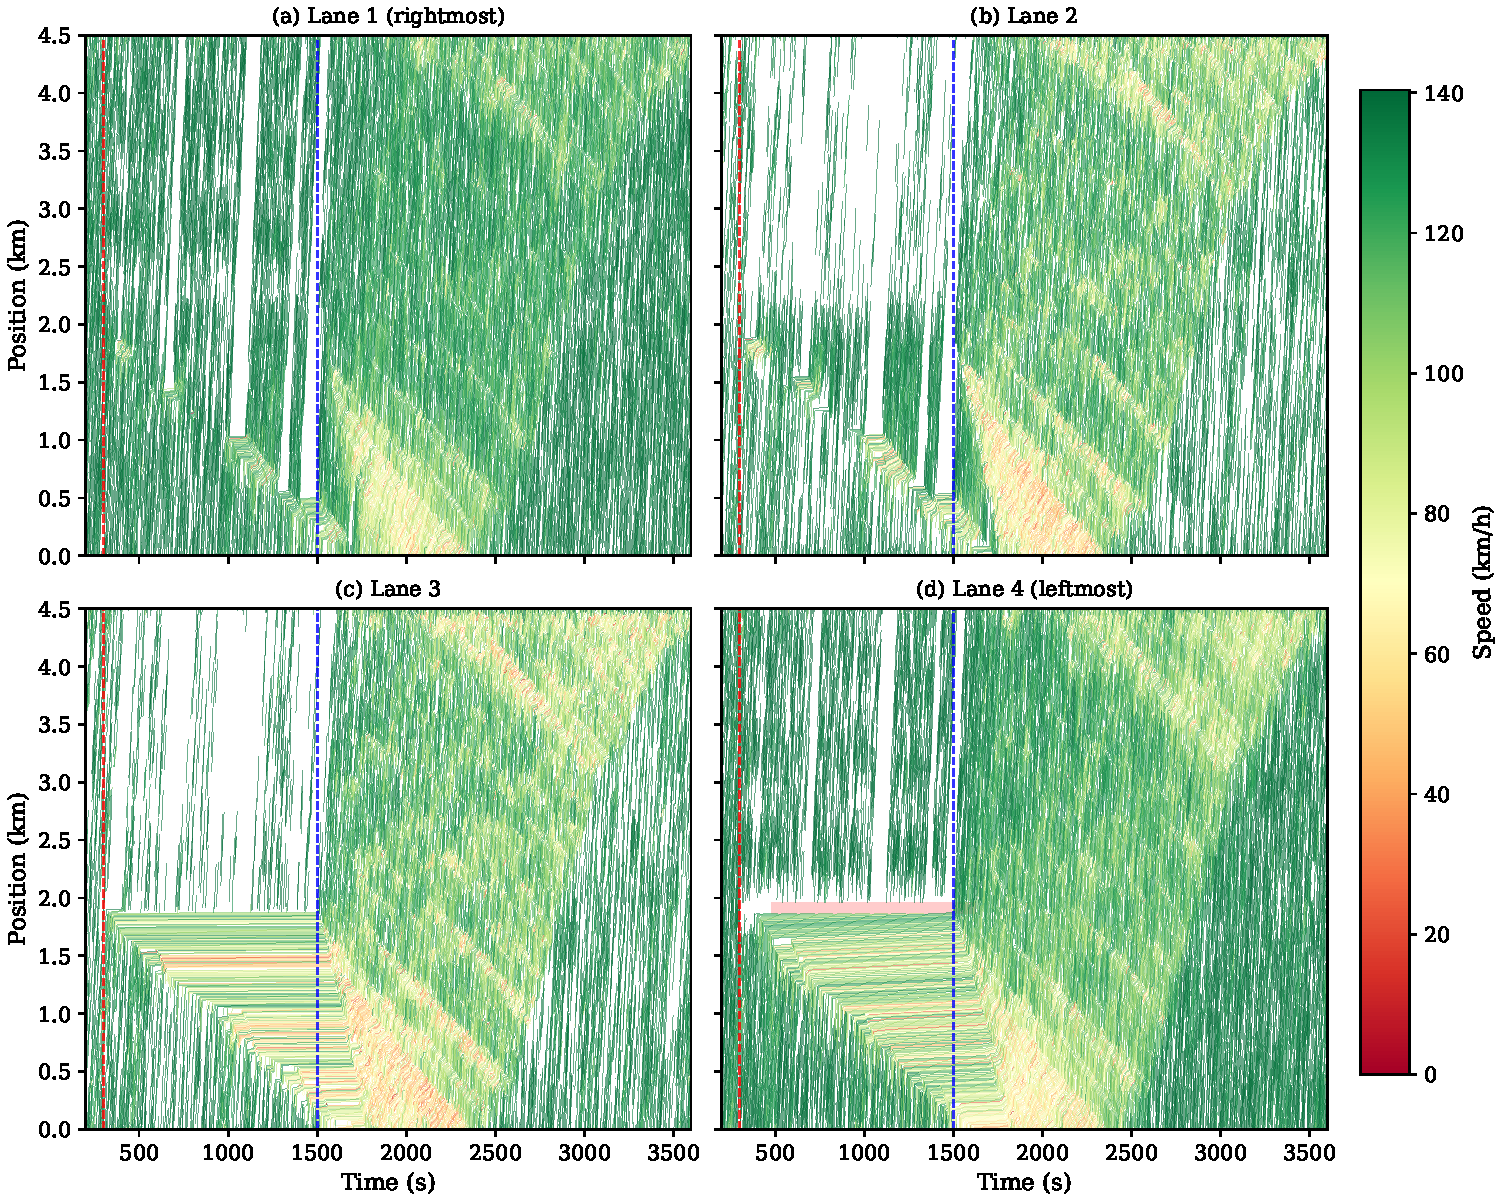
\includegraphics[width=\textwidth]{../figures/fig_incident_trajectories.pdf}
    \caption{Lane-by-lane time-space diagrams: baseline (left) vs.\ \DIFaddbeginFL \DIFaddFL{the }\DIFaddendFL 20-minute \DIFdelbeginFL \DIFdelFL{lane-closure incident }\DIFdelendFL \DIFaddbeginFL \DIFaddFL{closure of lanes~3 and~4 }\DIFaddendFL (right)\DIFaddbeginFL \DIFaddFL{, at 4}{\DIFaddFL{,}}\DIFaddFL{500\,veh/h}\DIFaddendFL . Trajectories are \DIFdelbeginFL \DIFdelFL{colored }\DIFdelendFL \DIFaddbeginFL \DIFaddFL{coloured }\DIFaddendFL by speed (green = free flow, red = stopped). Dashed lines on the incident panels mark \DIFdelbeginFL \DIFdelFL{incident }\DIFdelendFL onset ($t=300$\,s, red) and clearance ($t=1500$\,s, blue)\DIFaddbeginFL \DIFaddFL{, and the shaded band marks the blocked cells}\DIFaddendFL . The baseline \DIFdelbeginFL \DIFdelFL{shows uniform free-flow conditions}\DIFdelendFL \DIFaddbeginFL \DIFaddFL{is free-flowing throughout}\DIFaddendFL ; the incident panels show \DIFdelbeginFL \DIFdelFL{congestion buildup }\DIFdelendFL \DIFaddbeginFL \DIFaddFL{the blocked lanes emptying downstream, the queue growing upstream }\DIFaddendFL in all \DIFaddbeginFL \DIFaddFL{four }\DIFaddendFL lanes\DIFdelbeginFL \DIFdelFL{from merging traffic}\DIFdelendFL , \DIFdelbeginFL \DIFdelFL{with }\DIFdelendFL \DIFaddbeginFL \DIFaddFL{and the }\DIFaddendFL recovery \DIFaddbeginFL \DIFaddFL{spreading upstream }\DIFaddendFL after clearance.}
    \label{fig:incident_trajectories}
\end{figure}

Figure~\ref{fig:incident_heatmap} provides the corresponding lane-by-lane density heatmaps, mirroring the trajectory layout. The baseline columns (left) show uniform density throughout all lanes, confirming free-flow conditions at the given demand level. The incident columns (right) reveal the congestion dynamics per lane: \DIFdelbegin \DIFdel{lane}\DIFdelend \DIFaddbegin \DIFadd{lanes~3 and}\DIFaddend ~4 \DIFdelbegin \DIFdel{shows the direct impact of the closure zone}\DIFdelend \DIFaddbegin \DIFadd{hold the jam that forms against the blocked cells and are empty downstream of them}\DIFaddend , while lanes~\DIFdelbegin \DIFdel{1--3 exhibit progressively increasing density from merging traffic . Backward-propagating stop-and-go waves appear as }\DIFdelend \DIFaddbegin \DIFadd{1 and~2 take the merging traffic and carry the queue upstream with them. Within the queue, }\DIFaddend diagonal bands of high density \DIFdelbegin \DIFdel{within the congested region. The sharp boundary between congested and free-flow regimes is characteristic of }\DIFdelend \DIFaddbegin \DIFadd{run backwards in time-space, the stop-and-go waves of a congested stream; the boundary between the congested and free-flowing regions is sharp, as }\DIFaddend kinematic wave theory \DIFdelbegin \DIFdel{, and its emergence from }\DIFdelend \DIFaddbegin \DIFadd{predicts, and it emerges here from cells being released one reaction time after their holder moves on, with no macroscopic flow model anywhere in the simulation.
}

\DIFadd{After clearance the picture inverts: the bands tilt the other way, forwards, as the platoons discharged from the queue travel downstream at free-flow speed and spread out over the remaining kilometres of the segment. Upstream conditions return to the baseline 16 minutes after }\DIFaddend the \DIFdelbegin \DIFdel{resource-based simulation mechanics---without any macroscopic flow model---validates that the ODCA-DES framework faithfully reproduces first-order traffic dynamics at the macroscopic level while operating entirely at the microscopic, event-driven level. The slow recovery (approximately 25 minutes after clearance) reflects the hysteresis effect where the queue discharge rate initially falls below the arrival rate, consistent with empirical observations of incident recovery \mbox{%DIFAUXCMD
\citep{cassidy1998bivariate}}\hskip0pt%DIFAUXCMD
}\DIFdelend \DIFaddbegin \DIFadd{lanes reopen. The queue discharges more slowly than it formed, the reduced discharge capacity that empirical studies of active freeway bottlenecks report \mbox{%DIFAUXCMD
\citep{cassidy1999some}}\hskip0pt%DIFAUXCMD
}\DIFaddend .

\DIFdelbegin %DIFDELCMD < \begin{figure}[ht]
%DIFDELCMD <     %%%
\DIFdelendFL \DIFaddbeginFL \begin{figure}[htbp]
    \DIFaddendFL \centering
    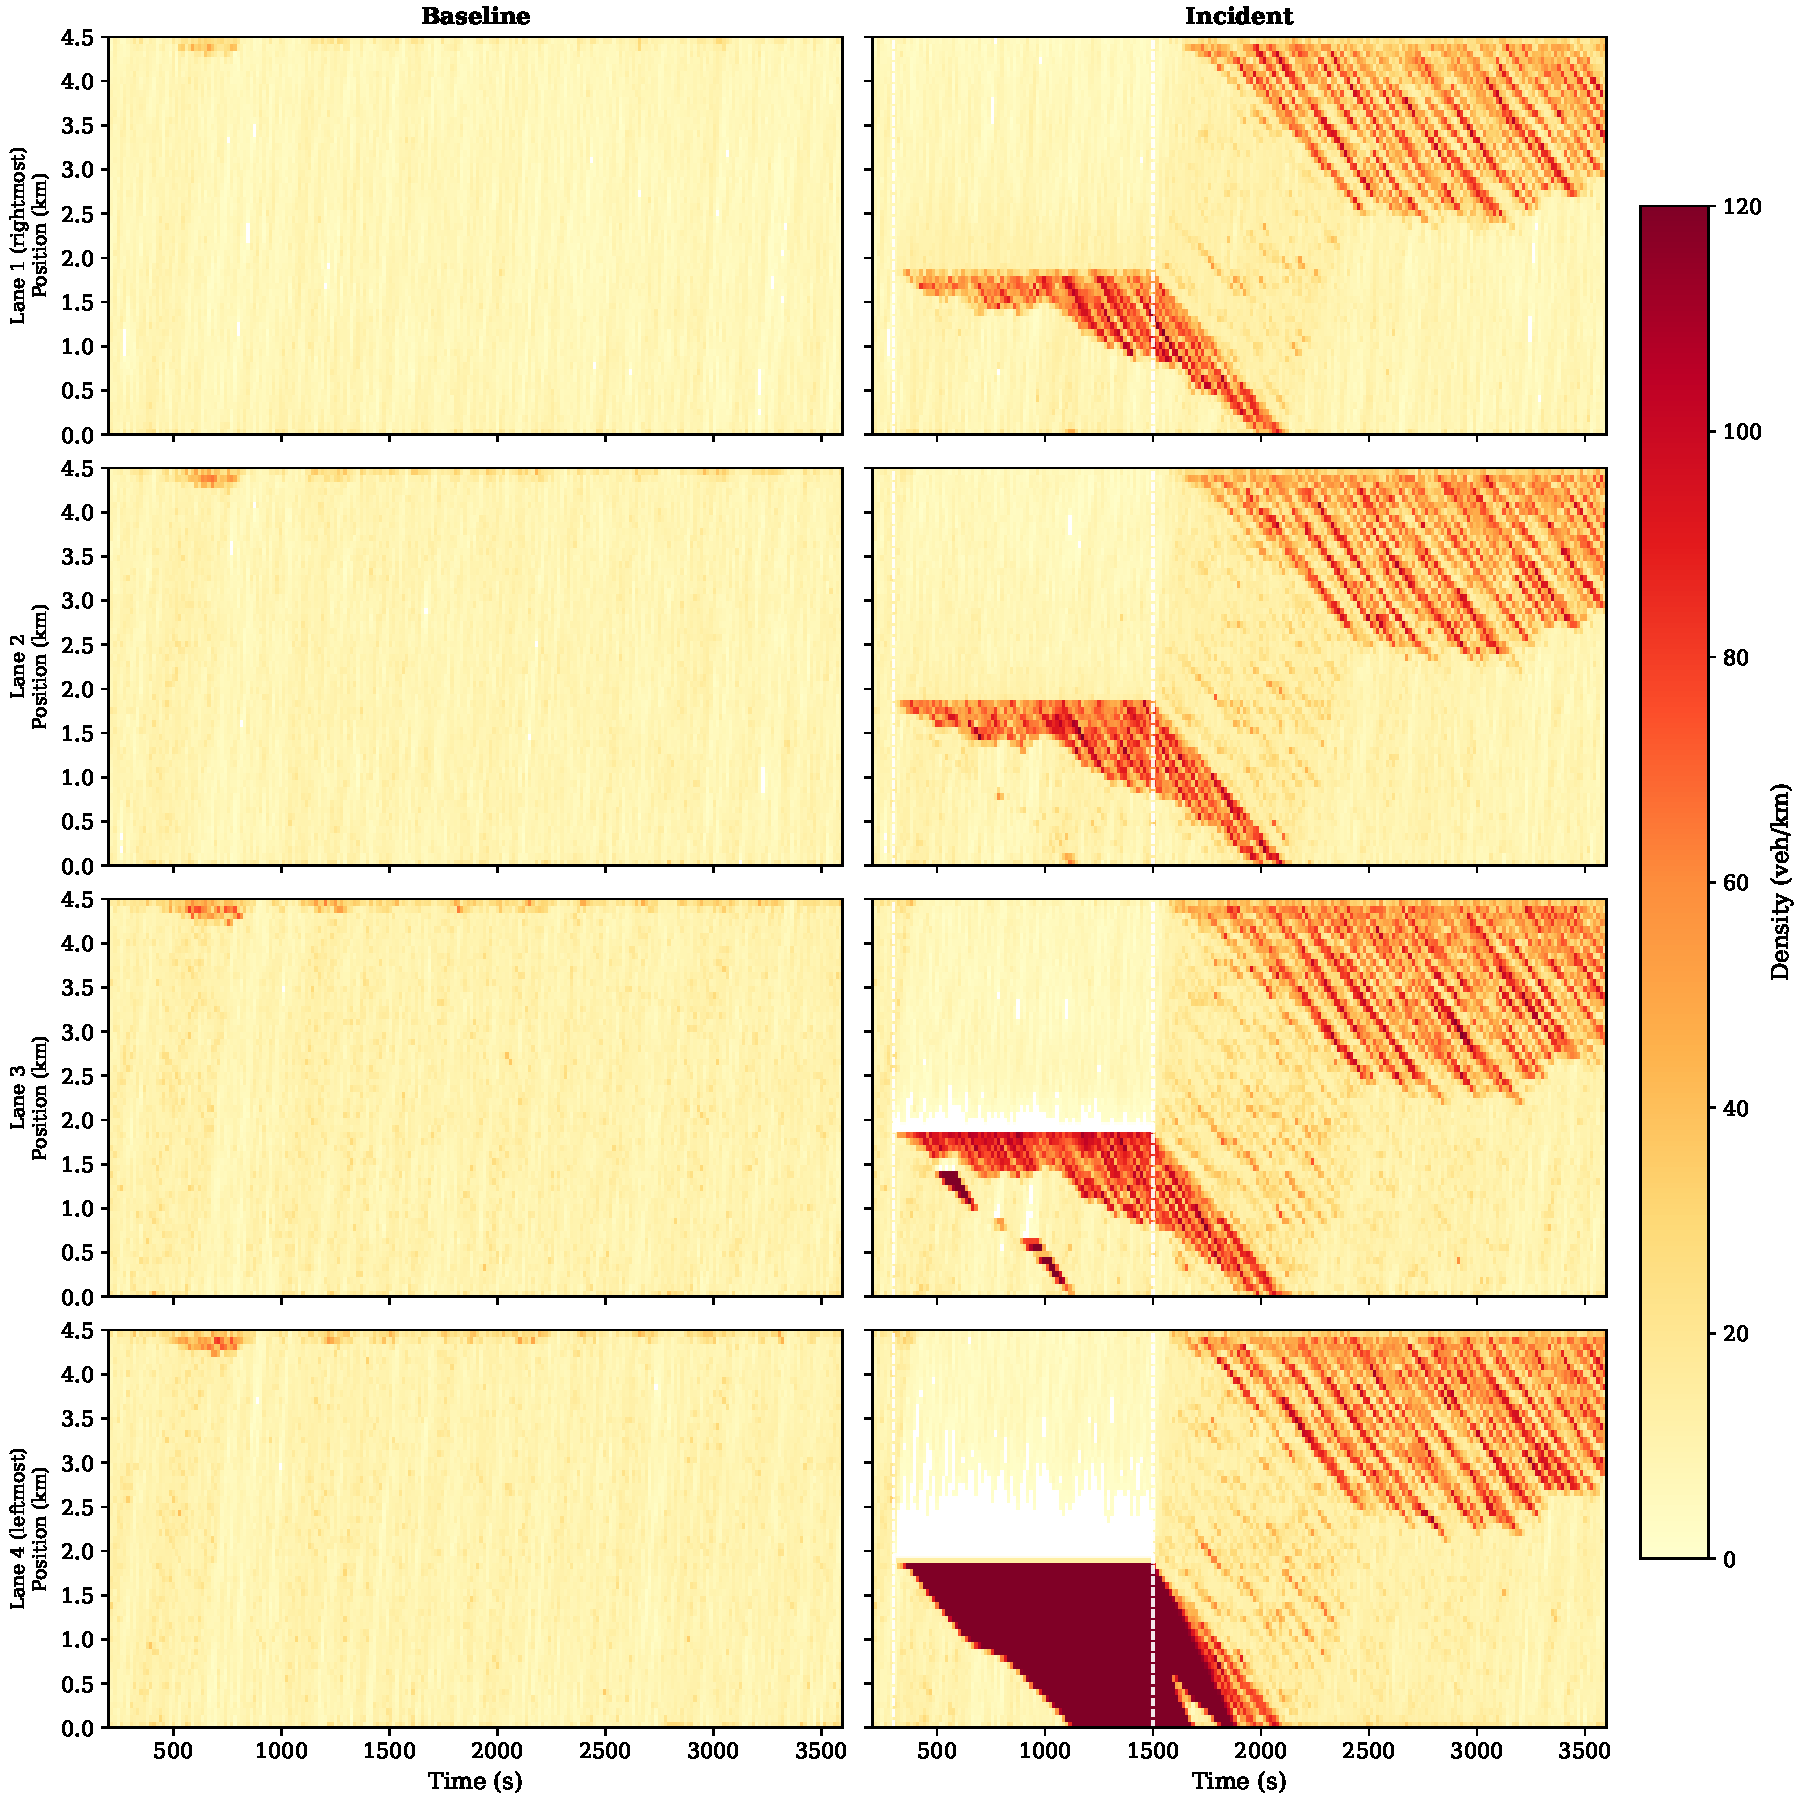
\includegraphics[width=\textwidth]{../figures/fig_incident_heatmap.pdf}
    \caption{Lane-by-lane time-space density heatmaps (15\,s $\times$ 75\,m bins): baseline (left) vs.\ \DIFaddbeginFL \DIFaddFL{the }\DIFaddendFL 20-minute \DIFdelbeginFL \DIFdelFL{lane-closure incident }\DIFdelendFL \DIFaddbeginFL \DIFaddFL{closure of lanes~3 and~4 }\DIFaddendFL (right). White dashed lines on the incident panels mark incident onset ($t=300$\,s) and clearance ($t=1500$\,s). The uniform baseline contrasts with lane-specific congestion patterns: lane~4 shows direct blockage impact, while lanes~1--3 show progressive density increases from merging traffic.}
    \label{fig:incident_heatmap}
\end{figure}


% ============================================================
\section{Conclusion}
\label{sec:conclusion}
% ============================================================

This paper presented the Object-Driven Cellular Automata (ODCA) framework within a Discrete Event Simulation environment for modeling multi-lane freeway traffic with heterogeneous vehicle populations. The key contributions are:

\begin{enumerate}
    \item A novel simulation paradigm that combines the spatial simplicity of cellular automata with the asynchronous, event-driven dynamics of discrete event simulation, eliminating the synchronous-update and integer-speed limitations of classical CA models.

    \item A resource-based movement protocol (request--wait--seize--delay--release) in which traffic congestion emerges naturally from cell resource contention, without explicit gap-checking or collision-avoidance rules.

    \item A delayed cell-release mechanism that produces headways consistent with Newell's simplified car-following model, establishing a direct analytical link between the simulation mechanics and traffic flow theory.

    \item A hybrid discretization scheme with discrete spatial cells, continuous vehicle speeds, and continuous event-driven time, yielding smooth fundamental diagrams and realistic trajectory outputs natively in the $T(x,n)$ passage-time coordinate system---a representation rarely exploited in simulation.

    \item An event-driven driver process where vehicles re-evaluate speed and lane-change decisions in response to neighbor movements rather than at fixed intervals, concentrating computational effort at locations where interactions occur and enabling immediate response to local density changes.

    \item Physically motivated lane-change safety assessment using speed-dependent closing-speed gaps and blockage-aware mandatory lane-change urgency inflation, producing realistic incident dynamics without requiring cooperative communication between vehicles.

    \item A decoupled architecture separating the driver process (speed and direction decisions) from the movement process (resource acquisition), enabling modular integration of heterogeneous behavioral models for mixed AV/HDV populations.

    \item A closed-form expression for the capacity effect of AV penetration (Eq.~\ref{eq:mixed_capacity}), derived directly from the resource protocol parameters, providing an analytical basis for assessing AV deployment scenarios.
\end{enumerate}

The analytical results established that the ODCA-DES framework produces a triangular fundamental diagram identical to that of Newell's kinematic wave model, with free-flow speed $v_f$ and backward wave speed $w = \ell/\tau$ emerging directly from the cell length and delayed-release parameters. The illustrative comparison with the NaSch model demonstrated that the event-driven, continuous-speed approach eliminates the integer-speed artifacts and artificial synchronization inherent in classical CA, while the resource-based conflict resolution provides a physically consistent and deadlock-free alternative to rule-based gap checking.

The event-driven driver process represents a fundamental departure from both classical CA and fixed-timestep microsimulators: vehicles re-evaluate their behavior in response to neighbor movements rather than at predetermined intervals, naturally producing adaptive evaluation frequencies that match the local interaction intensity. In free flow, a vehicle generates only periodic re-evaluations; in congestion, the same vehicle responds immediately to every neighbor movement. This push-based architecture, combined with speed-dependent closing-speed safety gaps and blockage-aware lane-change urgency inflation, produces physically realistic incident dynamics---including upstream spillback and post-clearance recovery---without requiring cooperative communication or centralized coordination among human-driven vehicles.

Computational experiments with 20 independent replications demonstrated the framework's ability to reproduce expected traffic dynamics across multiple scenarios. The fundamental diagram validation confirmed close agreement with the theoretical triangular FD\DIFaddbegin \DIFadd{: on a ring road, which removes the entry boundary effect, the simulated capacity reaches 92--93\% of the analytic $q_{\max}$}\DIFaddend , with scatter patterns arising from per-driver heterogeneity. Under increasing AV penetration from 0\% to 70\%, \DIFdelbegin \DIFdel{network }\DIFdelend \DIFaddbegin \DIFadd{served }\DIFaddend throughput increased by \DIFdelbegin \DIFdel{48}\DIFdelend \DIFaddbegin \DIFadd{18.9}\DIFaddend \% (from \DIFdelbegin \DIFdel{$4{,}494 \pm 14$ to $6{,}664 \pm 48$}\DIFdelend \DIFaddbegin \DIFadd{$5{,}874 \pm 19$ to $6{,}983 \pm 34$}\DIFaddend \,veh/h) and average delay decreased by \DIFdelbegin \DIFdel{89}\DIFdelend \DIFaddbegin \DIFadd{95}\DIFaddend \% (from \DIFdelbegin \DIFdel{$254 \pm 7$ to $28 \pm 1$}\DIFdelend \DIFaddbegin \DIFadd{$217 \pm 6$ to $10.2 \pm 0.3$}\DIFaddend \,s) on a congested 4-lane network with per-lane origin--destination flows. \DIFdelbegin \DIFdel{A lane-drop bottleneck experiment revealed that the throughput benefit of AV penetration plateaus near }\DIFdelend \DIFaddbegin \DIFadd{Both experiments show the same transition: once enough AVs are present for the network to serve the demand offered to it (99.8\% of 7}{\DIFadd{,}}\DIFadd{000\,veh/h at 70\% AV on the open freeway; 99.2\% of 3}{\DIFadd{,}}\DIFadd{600\,veh/h from }\DIFaddend 50\% \DIFdelbegin \DIFdel{, with }\DIFdelend \DIFaddbegin \DIFadd{AV at the lane drop and all of it at 70\%), throughput cannot record further capacity, and the benefit appears in delay, which falls by a further factor of three between }\DIFaddend the 50\% and 70\% \DIFdelbegin \DIFdel{AV scenarios producing statistically indistinguishable throughput ($1{,}773 \pm 164$ vs.\ $1{,}780 \pm 174$}\DIFdelend \DIFaddbegin \DIFadd{bottleneck scenarios ($18.1 \pm 2.1$ to $6.1 \pm 0.3$}\DIFaddend \,\DIFdelbegin \DIFdel{veh/h) ---a finding attributable to merge-capacity saturation at the 2-lane bottleneck throat}\DIFdelend \DIFaddbegin \DIFadd{s) whose throughputs are statistically indistinguishable}\DIFaddend . Sensitivity analysis showed that reducing the HDV action interval from 1.0\,s to 0.25\,s increases throughput by \DIFdelbegin \DIFdel{8.4\%, }\DIFdelend \DIFaddbegin \DIFadd{6.4\%, most of it in the first halving, }\DIFaddend quantifying the structural gap between the discrete-event implementation and the continuous-time theoretical limit. The temporary incident experiment showed that backward-propagating stop-and-go waves, congestion spillback, and gradual recovery emerge naturally from the event-driven resource protocol.

The event-driven architecture achieved real-time ratios of \DIFdelbegin \DIFdel{$1.2$}\DIFdelend \DIFaddbegin \DIFadd{$5.9$}\DIFaddend --\DIFdelbegin \DIFdel{$8.0\times$ }\DIFdelend \DIFaddbegin \DIFadd{$100\times$ }\DIFaddend on a single-threaded Python process (hardware as specified in Section~\ref{sec:exp_setup}) \DIFdelbegin \DIFdel{, with sub-linear event scaling }\DIFdelend across network sizes from 800 to 12{,}800 cells\DIFaddbegin \DIFadd{, with an event count that grew by 10.8 for a 16-fold increase in trip length}\DIFaddend . The DES paradigm's inherent event locality---where computational effort concentrates at congested locations and times---provides a foundation for future parallelization and large-network scalability that fixed-timestep approaches cannot match without significant algorithmic modification.

\subsection{Limitations}

Several limitations of the current framework should be noted:

\begin{itemize}
    \item \textbf{No empirical calibration.} All model parameters (reaction times, headway distributions, lane-change thresholds) are derived from representative values in the literature rather than calibrated to a specific field dataset. Validation against empirical trajectory data---such as NGSIM or highD---would require matching simulated and observed fundamental diagrams, headway distributions, and lane-change rates at specific sites. Until such calibration is performed, the quantitative predictions (absolute throughput, delay magnitudes) should be interpreted as framework demonstrations rather than site-specific forecasts.

    \item \textbf{Single unidirectional freeway segment.} The test network is a single straight freeway with on/off-ramps. There are no merge/diverge junctions, weaving sections, signalized ramp meters, or route-choice decisions. The resource-based architecture is in principle extensible to such geometries, but the current implementation does not support them.

    \item \textbf{Static demand.} All experiments use constant origin--destination flow rates. The event-driven architecture is compatible with time-varying demand---injection rates can be scheduled as time-dependent events---but the current implementation does not expose this capability. Consequently, the framework has not been tested under peak-hour demand ramps, demand shocks, or diurnal patterns.

    \item \textbf{Limited heterogeneity calibration.} While per-driver parameter sampling (LogNormal for $\tau$ and action interval, Normal for slowdown probability) introduces within-type heterogeneity, the distribution parameters are literature-derived rather than fitted to observed driver populations. Lane-change parameters remain homogeneous within each vehicle type.

    \item \textbf{Sensitivity scope.} The action-interval sensitivity analysis (Section~\ref{sec:exp_sensitivity}) covers only the all-HDV scenario (S1). Because the action interval is an HDV parameter and AVs operate on a fixed 10\,Hz controller cycle, the sensitivity is greatest in HDV-dominated traffic. At higher AV penetration levels, HDV behavioral parameters have proportionally less influence on aggregate performance. Extending the sensitivity analysis to mixed-traffic scenarios at low action intervals was computationally intractable within the experimental budget.

    \item \textbf{No creeping behavior.} When a vehicle's lane-change request cannot be immediately satisfied (target lane cell occupied), the vehicle stops in its current cell and waits. In reality, drivers ``creep'' forward, inching into gaps incrementally. Modeling creeping requires partial cell occupancy or multi-cell resource acquisition, which is a natural extension of the resource framework.
\end{itemize}

\subsection{Future Research Directions}

The ODCA-DES framework provides a foundation for several research directions:

\begin{itemize}
    \item \textbf{Empirical calibration and validation.} The $T(x,n)$ trajectory output format is well-suited for direct comparison with trajectory datasets such as NGSIM and highD, which provide vehicle-level passage times at discrete cross-sections. A systematic calibration study would fit the reaction-time, headway, and lane-change distributions to observed trajectory data at specific sites, enabling quantitative validation of the fundamental diagram shape, headway distributions, and congestion wave speeds.

    \item \textbf{Network-level extension.} The cell-based resource model can be extended to freeway networks by defining merge and diverge cells with multi-input or multi-output resource connections, enabling corridor-level simulations with interchanges, weaving sections, and route-choice decisions.

    \item \textbf{Time-varying demand.} The event-driven architecture is compatible with time-varying injection rates scheduled as time-dependent events. Implementing and validating this capability would enable simulation of peak-hour demand ramps, demand shocks, and diurnal traffic patterns.

    \item \textbf{Expanded sensitivity analysis.} Extending the action-interval sensitivity to mixed-traffic scenarios (S2--S4) would quantify the interaction between HDV behavioral granularity and AV penetration level. Computational advances (e.g., event batching or parallel DES engines) may be needed to make low-action-interval mixed-traffic runs tractable.

    \item \textbf{Calibrated driver heterogeneity.} Calibrating the per-driver parameter distributions against empirical driver-behavior data would produce more realistic traffic dynamics and enable the study of behavioral variability effects on traffic stability and capacity.

    \item \textbf{Creeping behavior.} Allowing vehicles to partially advance during lane-change waits would improve realism and throughput prediction, particularly at high-demand weaving sections.

    \item \textbf{Advanced AV coordination.} The decoupled architecture enables integration of cooperative AV behaviors (platoon formation, coordinated lane changes, V2V communication) as controller modules, without modifying the underlying movement engine.
\end{itemize}


% ============================================================
% References
% ============================================================
\bibliographystyle{elsarticle-harv}
\bibliography{references-marked}

\end{document}
